\documentclass[11pt]{article}

% --- Packages ---
\usepackage[usenames, dvipsnames]{color} % Cool colors
\usepackage{enumerate, amsmath, amsthm, amssymb, mathrsfs, algorithm, algpseudocode, pifont, subfig, fullpage, csquotes, dashrule, tikz, bbm, booktabs, bm, hyperref}
\usepackage[framemethod=TikZ]{mdframed}
\usepackage[numbers]{natbib}
\usepackage[normalem]{ulem}

% --- Misc. ---
\hbadness=10000 % No "underfull hbox" messages.
\setlength{\parindent}{0pt} % Removes all indentation.

% -- Commands --
% COMMANDS:
% - bigmid: Dynamically sized mid bar.
% - spacerule: add a centered dashed line with space above and below
% - \dbox{#1}: Adds a nicely formatted slightly grey box around #1
% - \begin{dproof} ... \end{dproof}: A nicely formatted proof. Use \qedhere to place qed
% - \ddef{#1}{#2}: Makes a definition (and counts defs). #1 goes inside parens at beginning, #2 is actual def.
% - \begin{dtable}{#1} ... \end{dtable}: Makes a minimalist table. #1 is the alignment, for example: {clrr} would be a 4 column, center left right right table.

% Dynamically sized mid bar.
\newcommand{\bigmid}{\mathrel{\Big|}}


% ---- Colors and Notes ----
\definecolor{dblue}{RGB}{98, 140, 190}
\definecolor{dlblue}{RGB}{216, 235, 255}
\definecolor{dgreen}{RGB}{124, 155, 127}
\definecolor{dpink}{RGB}{207, 166, 208}
\definecolor{dyellow}{RGB}{255, 248, 199}
\definecolor{dgray}{RGB}{46, 49, 49}

% TODO
\newcommand{\todo}[1]{\textcolor{red}{TODO: #1}}
\newcommand{\dnote}[1]{\textcolor{dblue}{Dave: #1}}

% URL
\newcommand{\durl}[1]{\textcolor{dblue}{\underline{\url{#1}}}}

% Circled Numbers
\newcommand*\circled[1]{\tikz[baseline=(char.base)]{\node[shape=circle,draw,inner sep=0.7pt] (char) {\footnotesize{#1}};}}
% From: http://tex.stackexchange.com/questions/7032/good-way-to-make-textcircled-numbers

% Under set numbered subset of equation
\newcommand{\numeq}[3]{\underset{\textcolor{#2}{\circled{#1}}}{\textcolor{#2}{#3}}}

% ---- Abbreviations -----
\newcommand{\tc}[2]{\textcolor{#1}{#2}}
\newcommand{\ubr}[1]{\underbrace{#1}}
\newcommand{\uset}[2]{\underset{#1}{#2}}
\newcommand{\eps}{\varepsilon}

% Typical limit:
\newcommand{\nlim}{\underset{n \rightarrow \infty}{\lim}}
\newcommand{\nsum}{\sum_{i = 1}^n}
\newcommand{\nprod}{\prod_{i = 1}^n}

% Add an hrule with some space
\newcommand{\spacerule}{\begin{center}\hdashrule{2cm}{1pt}{1pt}\end{center}}

% Mathcal and Mathbb
\newcommand{\mc}[1]{\mathcal{#1}}
\newcommand{\indic}{\mathbbm{1}}
\newcommand{\bE}{\mathbb{E}}

\newcommand{\ra}{\rightarrow}
\newcommand{\la}{\leftarrow}

% ---- Figures, Boxes, Theorems, Etc. ----

% Basic Image
\newcommand{\img}[1]{
\begin{center}
\includegraphics[\width=0.6\textwidth]{#1}
\end{center}}

% Put a fancy box around things.
\newcommand{\dbox}[1]{
\begin{mdframed}[roundcorner=4pt, backgroundcolor=gray!5]
\vspace{1mm}
{#1}
\end{mdframed}
}

%  --- PROOFS ---

% Inner environment for Proofs
\newmdenv[
  topline=false,
  bottomline=false,
  rightline = false,
  leftmargin=10pt,
  rightmargin=0pt,
  innertopmargin=0pt,
  innerbottommargin=0pt
]{innerproof}

% Proof Command
%\newenvironment{dproof}{\begin{proof} \text{\vspace{2mm}} \begin{innerproof}}{\end{innerproof}\end{proof}\vspace{4mm}}
\newenvironment{dproof}[1][Proof]{\begin{proof}[#1] \text{\vspace{2mm}} \begin{innerproof}}{\end{innerproof}\end{proof}\vspace{4mm}}


% Dave Definition
\newcounter{DaveDefCounter}
\setcounter{DaveDefCounter}{1}

\newcommand{\ddef}[2]
{
\begin{mdframed}[roundcorner=1pt, backgroundcolor=white]
\vspace{1mm}
{\bf Definition \theDaveDefCounter} (#1): {\it #2}
\stepcounter{DaveDefCounter}
\end{mdframed}
}

% Block Quote
\newenvironment{dblockquote}[2]{
\begin{blockquote}
#2
\vspace{-2mm}\hspace{10mm}{#1} \\
\end{blockquote}}

% Algorithm
\newenvironment{dalg}[1]
{\begin{algorithm}\caption{#1}\begin{algorithmic}}
{\end{algorithmic}\end{algorithm}}




% Dave Table
\newenvironment{dtable}[1]
{\begin{figure}[h]
\centering
\begin{tabular}{#1}\toprule}
{\bottomrule
\end{tabular}
\end{figure}}

% For numbering the last of an align*
\newcommand\numberthis{\addtocounter{equation}{1}\tag{\theequation}}

\DeclareMathOperator*{\argmin}{arg\,min}
\DeclareMathOperator*{\argmax}{arg\,max}

\newtheorem{conjecture}{Conjecture}[section]
\newtheorem{remark}{Remark}[section]
\newtheorem{theorem}{Theorem}[section]
\newtheorem{corollary}{Corollary}[theorem]
\newtheorem{lemma}[theorem]{Lemma}
\newtheorem{assumption}{Assumption}


\title{AAAI 2019 Notes \\ \Large{Honolulu, HI, USA}}
\author{David Abel\footnote{\durl{http://david-abel.github.io\textasciitilde dabel}} \\ \durl{david_abel@brown.edu}}
\date{January \& February 2019}

\begin{document}
\maketitle
\tableofcontents
\newpage


This document contains notes I took during the events I managed to make it to at AAAI in Honolulu, Hawaii, USA, including sessions of the the doctoral constortium. Please feel free to distribute it and shoot me an email at \durl{david_abel@brown.edu} if you find any typos or other items that need correcting.

% ------------
% -- Sunday --
% ------------
\section{Sunday January 27th}
It begins! Today I'll be at the Doctoral Consortium (DC) -- my goal with the notes is both to give folks a sense of what a DC entails, and to share the exciting research of some great grad students. \\

\subsection{Neeti Pokhriyal: Multi-View Learning From Disparate Sources for Poverty Mapping}

{\bf Focus:} Learning from multiple disparate data sources, applied to sustainability and biometrics. \\

Specific Application: Povert mapping. Spatial representation of economic deprivations for a country. A major tool for policy planners. \\

Current method is a household survey, which is 1) costly, 2) time consuming, 3) only available for small samples. \\

{\bf Research Goal:} Get accurate, spatially detailed and diagnostic poverty maps for a country. \\

Lots of data available via weather, street maps, economic data, mobile phones, satellite imagery. But! Each of these data sources are structured very different. \\

\begin{figure}[h!]
    \centering
    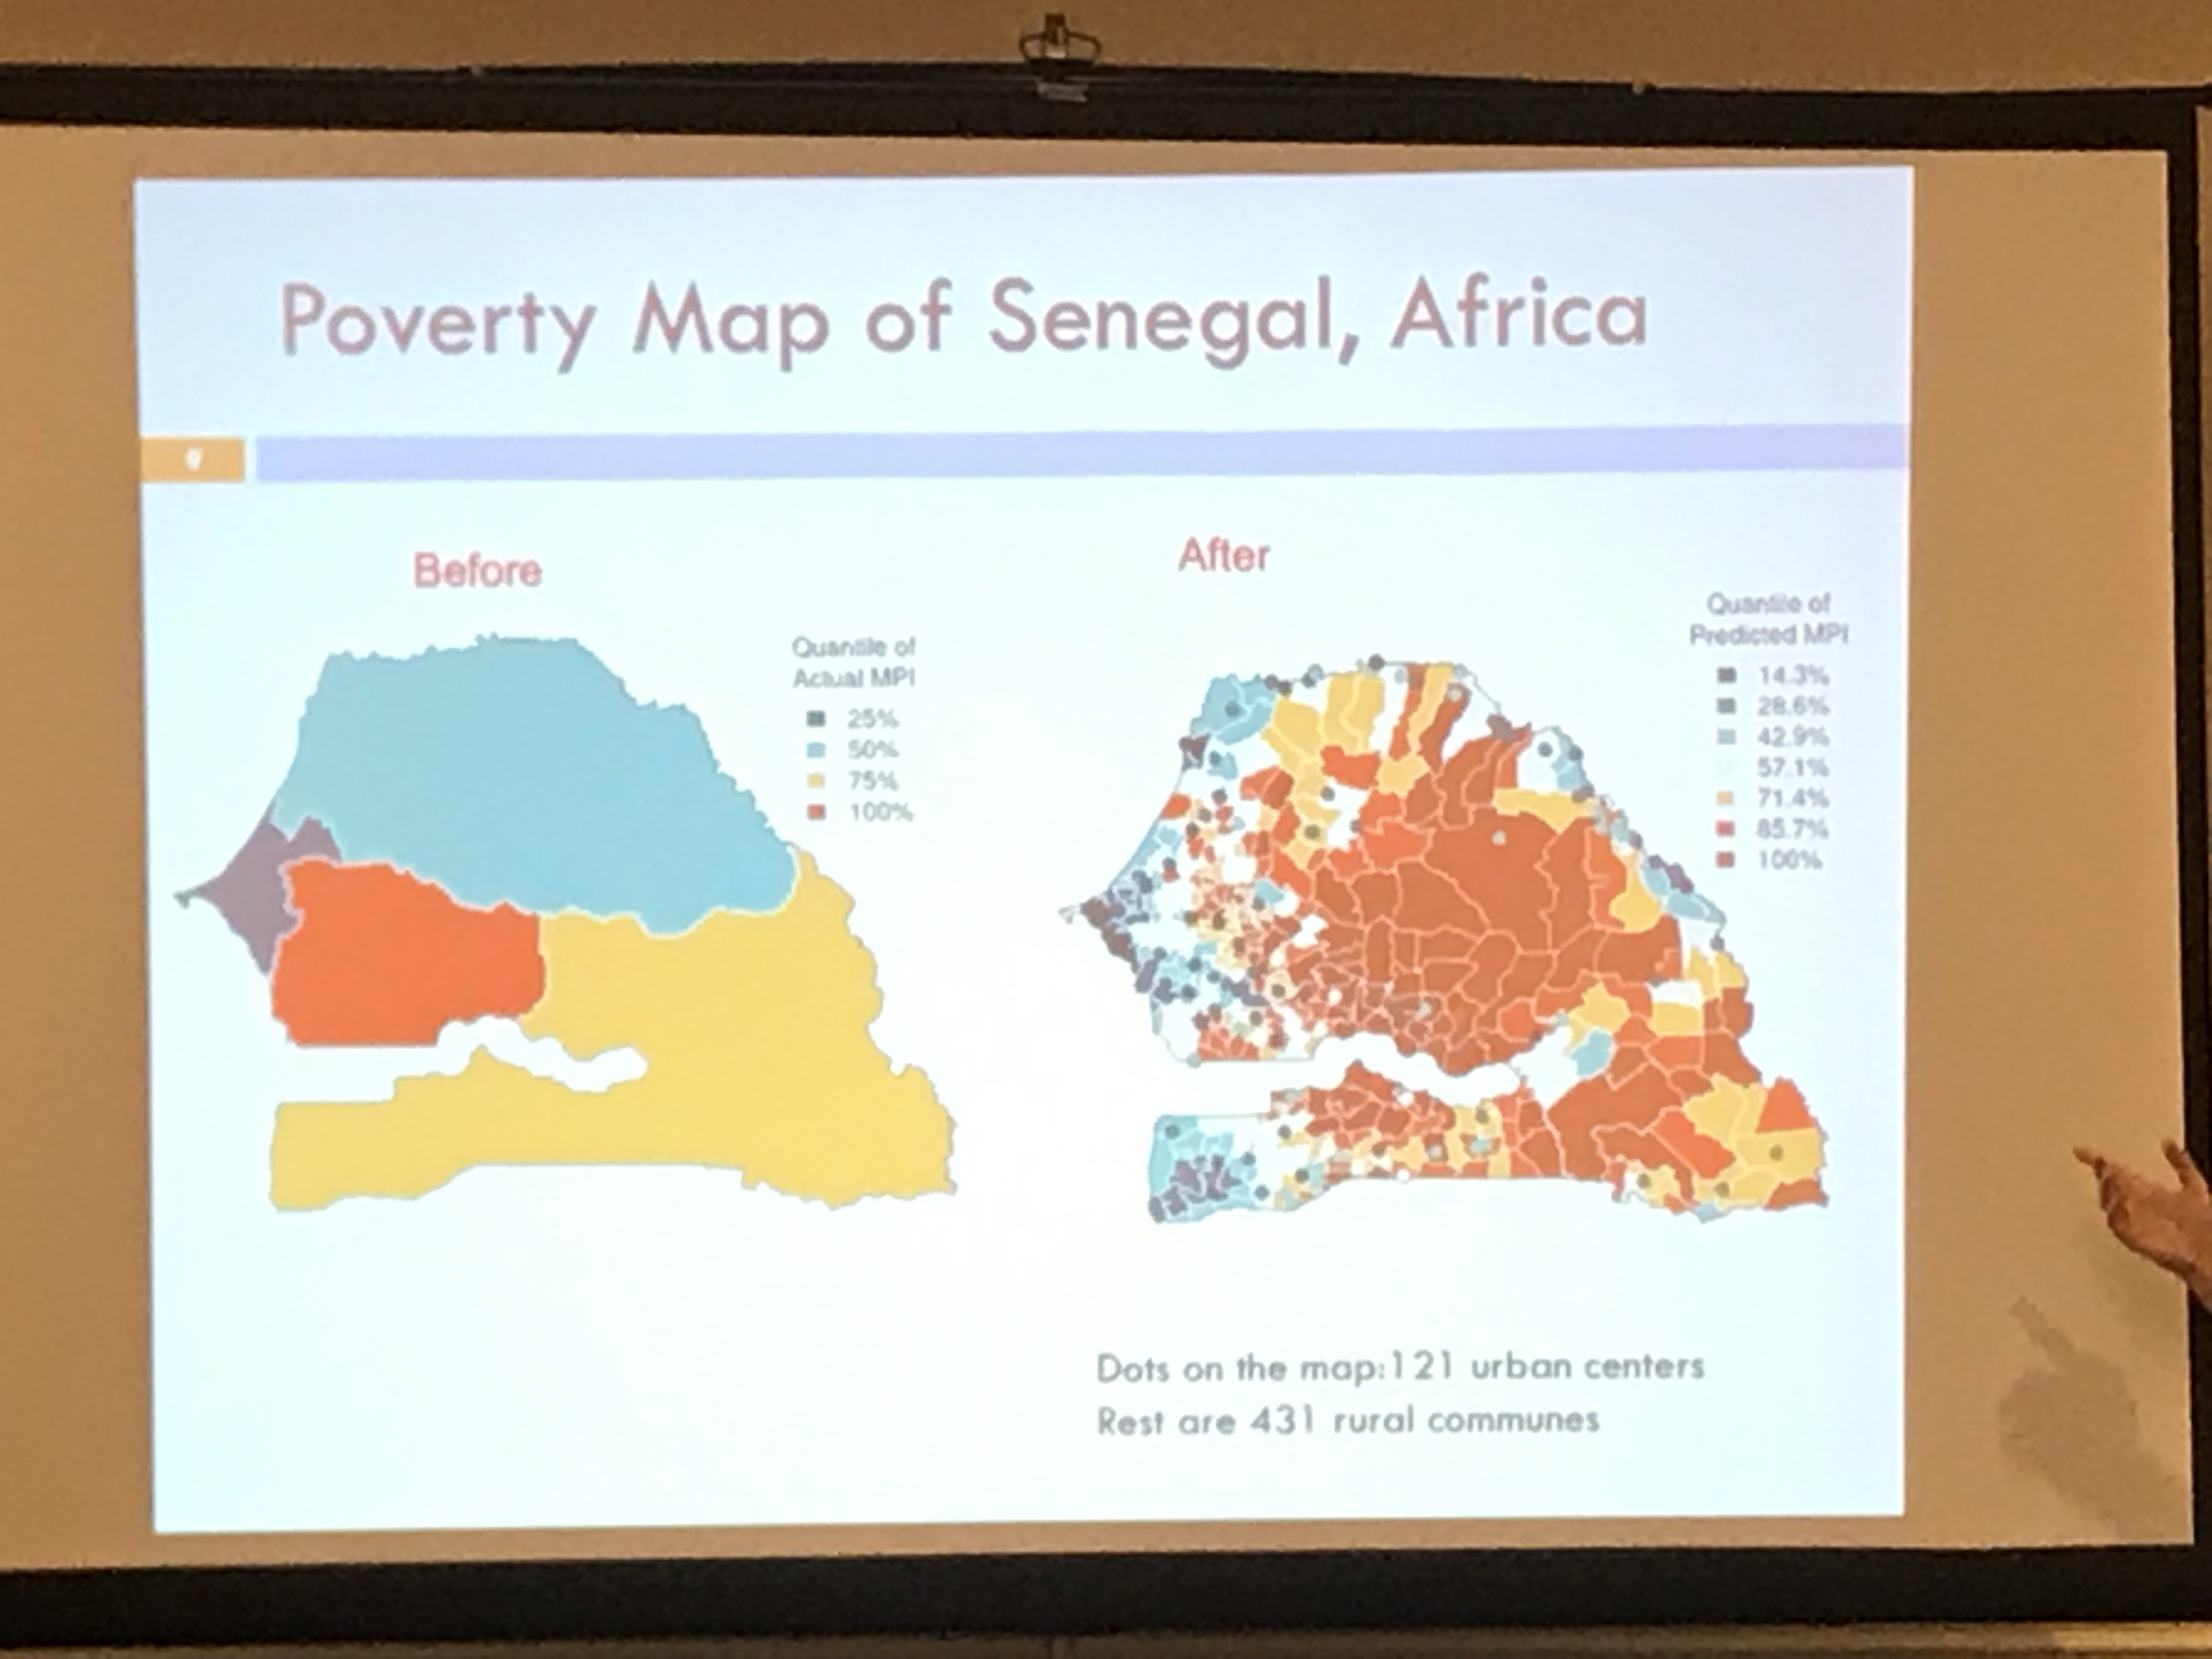
\includegraphics[width=0.5\textwidth]{images/pov_map.JPG}
    \caption{Higher fidelity poverty prediction}
    \label{fig:pov_map}
\end{figure}

\ddef{Multi-View Learning}{A style of learning takes as input separate, semantically distinct kinds of data, and brings them together into a factorized representation for use in predictive models.}

Method: learn a Gaussian Process (GP) Regression model combined with elastic net regulariation~\cite{zou2005regularization}. \\

Using this model yields the map pictured in Figure~\ref{fig:pov_map}. Then perform quantitive analysis and validates that their model is making high quality predictions by comparing to census data. \\

{\bf Objective 2:} learn a factorized representation from multiple data sources. The hope is that we can disentangle explanatory factors that are unique to each data source. \\

Sort of an EM like approach:
\begin{enumerate}
    \item {\it Learning Step:} MAp views $Y$ and $Z$ to shared subspaces $X_i, \ldots$.
    \item {\it Inference Step:} Perform inference on these subspaces.
\end{enumerate}

Q: Main question, then: how do we learn the shared subspace?\\

A: Separate data belonging to different class across different views is maximized, while ensuring alignment of projects from each view to the shared space. Can be solved using a Generalized Eigenvalue problem, or using the kernel trick.



\spacerule
\subsection{Negar Hassanpour: Counterfactual Reasoning for Causal Effect Estimation}

{\bf Problem:} Consider Mr. Smith, who has a disease and some known properties (age, BMI, etc.). Doctor provides treatment X and observes the effect of treatment X (but does {\it not} get data about the counterfactul: what would have happened if doc had applied treatment Y?). \\

{\bf Goal:} Estimate the ``Individual Treatment Effects" (ITE) -- how does treatment X compare to Y? \\

Datasets:
\begin{itemize}
    \item Randomized Controlled Trial (RCT): See lots of both X and Y. But, it's expensive (lots of trials) and unethical (giving placebos when you know the right treatment).
    \item Observational Study: provide the preferred treatment. But, sample selection bias.
    
    {\it Example:} Treating heart disease, a doc prescribes surgery to younger patients and medication to older patients. Compare survival time -- but, clear bias in who gets what treatment.
\end{itemize}

This is a really fundamental problem called ``sample selection bias" -- rich patients receiving expensive treatment vs. poor patients receiving cheap treatment and so on. \\

Overview of this work:
\begin{itemize}
    \item Generate realistic synthetic datasets for evaluating these methods (since good data is hard to come by)
    
    $\ra$ Take an RCT and augment it with synthetic data.
    
    \item Use representation learning to reduce sample selection bias.
    
    $\ra$ Want $Pr(\phi(x) \mid t=0) \approx Pr(\phi(x) \mid t=1)$ to be similar, with $\phi$ the learned representation and $t$ the treatment.
    
    \item Learn underlying causal mechanism with generative models.
    
    $\ra$ Learn causal relationships between treatments and outcomes by using generative models. Can we identify the latent sources of outcome from observational dataset?
    
    \item Perform survival predictions.
    
    $\ra$ Can we predict outcomes that are censored or take place after studies end?
    
    \item Going beyond binary treatments
    
    $\ra$ Many, but not all, treatments are binary. Can we go beyond this to categorical or real valued treatments?
    
    \item Providing a course of treatment
    
    $\ra$ Call on reinforcement learning.

\end{itemize}



\spacerule
\subsection{Khimya Khetarpal: Learning Temporal Abstraction Across Action \& Perception}

Q: How should an AI agent efficiently represent, learn, and use knowledge of the world? \\

A: Let's use temporal abstractions! \\

Example: preparing breakfast. Lots of subtasks/activities involved like (high level): choose eggs, type of toast (mid level) chop vegetables, get butter, and (low level) wrist and arm movements. \\

\ddef{Options~\cite{sutton1999between}}{An option formalizes a skill/temporally extended action as a triple: $\langle, I, \beta, \pi \rangle$, where $I \subseteq S$ is a initiation set, $\beta : S \ra \Pr(S)$ is a termination probability, and $\pi : S \ra A$ is a policy.}

Example: A robot navigates through a house between two rooms. To do so, it has to open a door. We let $I$ denote the states where the door is closed, $\beta$ is 1 when the door is open and 0 otherwise, and $\pi$ opens the door. Then, this option defines the ``open the door" skill. \\

{\bf Main Question}: Can we learn useful temporal abstractions? \\

{\bf Hypothesis:} Learning options which are specialized in situations of specific interest can be used to get the right temporal abstractions. \\

Motivation: AI agents should be able to learn and develop skills continually, hierarchically, and incrementally over time. \\

So, imagine we had a house decomposed into different rooms. Then we would like to learn skills that take the agent between each room. Further, the agent should be able to transfer for one agent to another. \\

{\bf Objective 1:} Learn options and interest functions simultaneously. \\

New idea: break the option-critic assumption~\cite{bacon2017option} that $I = S$. Instead, consider an interest function:
\ddef{Interest Function}{An interest function is an indication of the extent to which an option is interested in state $s$.}

Now learn a policy over options and an interest function -- we can jointly optimized over both things. Derive the policy gradient theorem for interest functions, intra-option policy, and the termination function. \\

\begin{figure}[h!]
    \centering
    \includegraphics[width=0.5\textwidth]{images/four_room.png}
    \caption{Learned interest functions}
    \label{fig:opt_four}
\end{figure}

Also explore learning interest functions in continuous control tasks, showing nice separation between the learn options. \\

{\bf Objective 2:} Consider a never-ending stream of perceptual data. We'd like to learn a stream of percepts and behavior over time. \\

Challenges:
\begin{itemize}
    \item How can we the agent automatically learn features which are meaningful pseudo rewards?
    \item Where to task descriptions come from?
    \item How can we achieve the most general options without hand designing tasks/rewards?
    \item Evaluation in a lifelong learning task? Benchmarks?
\end{itemize}


\spacerule
\subsection{Ana Valeria Gonzalez-Garduño: RL for Low Resource Dialogue Systems}

{\bf Goal 1:} Create more informed approaches to dialogue generation. \\

{\bf Goal 2:} Use RL for domain adaption in goal oriented dialogue. \\

(And: can we do this in a language agnostic way? So, introduce models that can work with any/many languages). \\

Dialogue systems are divided into two subfields:
\begin{enumerate}
    \item {\it Open ended dialogue generation:} typically use encoder-decoder architectures
    \item {\it Goal oriented dialogue:} predominantly tackle using ``pipeline" methods. So, automatic speech recognition unit, then an understanding unit, and so on.
\end{enumerate}

Current Focus: ``state tracking". That is, state tracking deals with inferring the user intent or belief state during the conversation. \\

But, limitation: intents usually rely on a particular ontology that defines which intents are valid. \\

Current Status of the Project: Bridge the gap inb goal oriented dialogue. Main goal: can we get rid of the need for annotations? \\

General idea: given a bot's utterance (``how can I help?"), and a user response (``I want to change payment methods"), we want to find a relevant query from prior conversations to identify what the user said. Or really, use it to condition the decoder. \\

Result: this model works very well! On BLEU their model performs favorably, but more importantly, on a human evaluation, their responses were consistently chosen over the baseline. \\

Q: But, what if our domain is not in the pool of relevant conversations? \\

A: Work in progress! Idea $\ra$ Use RL:
\begin{enumerate}
    \item Phase 1: Use existing data for state tracking, pretrain models in a supervised manner.
    
    $\ra$ Turn level supervision, slots and values represented using word embeddings.
    
    \item Phase 2: Use RL to finetune pretrained model.
    
    $\ra$ Rely on dialogue level supervision (joint goal accuracy) as reward. So, how many slot-values (``Food-Mexican, Price-Cheap"), to determine the reward.
\end{enumerate}

Challenges in using RL for state tracking: dialogue is long (credit assignment is hard!), sample efficiency, might be able to leverage curriculum learning. \\

Main Future Direction: Enable dialogue state transition model to generate new unseen slots.


\spacerule
\subsection{AAAI Tutorial: Eugene Freuder on How to Give a Talk}


Start with an example! Or a counter example. \\

These are just his conclusions! So decide for yourself, of course. \\

This talk is not intended to be mean spirited -- he'll be talking about mistakes people make. \\

Meta-message: presenting a talk is a skill that can be studied and practiced! And it's worth doing -- spend years researching and 10 minutes presenting. The 10 minutes should be polished. \\

Six Points:
\begin{enumerate}
    \item Convey Enthusiasm
    \item Make it Easy to follow
    \item Employ examples
    \item Expressive
    \item Enhance your presentation with visuals/dynamic material
    \item Engage the audience
\end{enumerate}


\subsubsection{Enthusiasm}
The secret of a good talk: {\bf Enthusiasm!}\\

$\ra$ If you're not enthusiastic about your work, how do you expect anyone else to be? \\

Fear of public speaking: ``glausophobia" -- ranked as the most common fear in the USA (more so than spiders/death). \\

Q: How do you get over this fear? \\

A: Remember the audience is on your side! Breathe. Drink water. \\

Tricks:
\begin{itemize}
    \item Look over their heads (instead of in their faces-- can be easier).
    \item Or, turn it into an individual conversation, or a bunch of individual conversations.
    \item Science is fun! So have fun.
\end{itemize} 

Sometimes it feels like there's the me giving the talk and the me monitoring me giving the talk. Unfortunate, potentially, as I'm then not present.\\

It is {\bf really} hard to be too enthusiastic. The speaker is standing on a chair to demonstrate enthusiasm --\\


\subsubsection{Easy to Follow}

One major goal of the talk: get people to read and build on your work. Details are in the paper-- job in the talk is to get them to read the paper. \\

KISS principle: Keep It Simple Stupid! \\

Story from Feynman's lost lecture: someone asked Feynman to prepare a lecture on some complicated physics concept related to particle spin. Feynman said he would go off and work on it for a few days and come back and give a lecture: ``I'll be able to give a freshmen level lecture in a few days!". But then he came back: ``Okay, I couldn't do it. I couldn't turn it into a freshmen level lecture. {\it Which means we don't yet understand it yet}." \\

Audience doesn't distinguish hard work from the researcher having a hard time explaining it. \\

Let them see the forest -- not the trees. \\

Explain math/formalisms with visuals and metaphor. Minimize definitions, don't overestimate audience. \\

People make talks too difficult by going through material too quickly, or trying to force too much in. Time yourself!

\subsubsection{Use Examples}

Start with an example! Even before the title/introduction. \dnote{Hm! Bold move. Hard to do this in a conference, to me. But it's a neat idea.} \\

He played a clip from a TED talk (Niri G?) where the speaker opened just with ``Two twin domes...". It was engaging. \\

Even if you don't start with one -- use one. It can be hard to make the example simple enough. \\

Make your example(s):
\begin{itemize}
    \item Illustrate what you've done
    \item Simple
    \item Concrete
    \item Only add complexity later (or use a running example!)
\end{itemize}

\subsubsection{Be Expressive}

Use your voice and body language to be expressive. \\

Do's and Dont's:
\begin{itemize}
    \item[{\bf Do:}]  smile (he played Nat King Cole!), listen to yourself beforehand (and look for ``ums", body swaying, etc), try to make it a conversation (not a declamation), vary your voice (louder/softer, higher/lower), pause occasionally, articulate, look people in the eye, turn off your phone, silence computer.
    
    \vspace{4mm}
    
    \item[{\bf Don't:}] Read from a prompt, speak in a monotone, speak too fast or too slow, be distracting (like playing with your hair, rocking back and forth or front to back $\ra$ a good alternative is to hang onto the lectern), say ``um"/``uh" too much, mumble, fidget, turn around a face the screen, look at your laptop too much.
\end{itemize}

\subsubsection{Enhance your talk with visuals/dynamics}

Do's and Dont's:
\begin{itemize}
    \item[{\bf Do:}] use visuals, minimize text, keep notes for yourself, remember short term memory of audience (repeat details, highlight big things, etc.), pull out what is important. 
    \vspace{4mm}
    
    \item[{\bf Don't:}] use bulleted lists.
\end{itemize}

\subsubsection{Engage the Audience}

Q: How do you engage an audience directly? \\

A: Ask questions! \\

Consider why your audience is here: they want to hear what you did. Tell them right away what you're going to do. Big results at the beginning. \\

Can turn your talk into a story:
\begin{itemize}
    \item A problem to be solved. Someone came to me in a company with a problem, and so on.
    \item Could be the ``2x2 matrix" story: folks have done Red things and Blue things, and folks have done Small things and Big things, but no one has done Big Red things! I'm going to do that.
    \item Could contradict conventional wisdom
    \item The ``journey" and not just the endpoint.
\end{itemize}

Make your talk fun! ``A spoonful of sugar makes the medicine go down." Use gimmicks, like: playing songs, use props, video, etc. \\

Hypothesis: on average, at a CS conference, by the time you reach the halfway point, at least half the people would be tuned out. \\

$\ra$ So: if the hypothesis is even close to being right, think of the waste! \\

\subsection{Aida Rahmattalabi: Robust Peer-Monitoring on Graphs}

{\bf Problem:} Suicide is a critical public health problem in the US. Second leading cause of death among students. \\

One approach: gatekeeper training (suicide prevention program). Can identify warning signs, but can only train limited number of individuals. \\

{\bf Main Goal:} Improve gate keeper training with social network information by taking into account characteristics of individals in the population. \\

Technical problem: optimize:
\begin{equation}
    \max_{x,y} \sum_{n \in N} y_n,
\end{equation}
subject to $x \in \mc{X}$ and $y \in \mc{Y}$, which define the feasible sets of possible choices of trainers. \\

Basically: social characteristics are very important in assigning a gatekeeper. So, impose constraints on who is chosen as a gatekepeer (based on things like race/gender). \\

But, new problem: participation uncertainty. Not all chosen trainers might not participate. \\

Optimization problem is formulated as:
\begin{equation}
    \max_{x \in \mc{X}} \min_{\eps \in E} \sum_{n \in N} y_n(x,\eps),
\end{equation}
where the $x$ is the gatekeeper we choose, and natre is acting adversarially over choice of $\sigma$ which determines participation rate. $y_n(x,\epc)$ denotes the coverage for each of the $n$ individuals. Can cast this as a polynomial size mixed integer program which is nice and tractable. That is, main result:
\begin{theorem}
For a fixed vale of $K$, their main optimization problem (the ``$k$ adaptibility problem"), can be reformulated exactly as a polynomially sized mixed integer linear program.
\end{theorem}

Experiments: compare to a greedy robust approach on a real social network. Measuring ``coverage", which is captured by the function $y$ above. Also evaluate according to a ``Price of Fairness".


\subsection{Nikhil Bhargava	: Multi-Agent Coordination under Uncertain Communication}

Consider under water gliders: they go underwater for months at a time, so we can't actually communicate with them very often.\\

So, most folks usually use a ``real time executive" (RTE), which is a centralized, real-time means of dispatching actions to different agents. \\

But: in reality, too much uncertainy in action execution. So, RTEs often include state updates based on the outcome of action executions. \\

Lots of prior work on RTEs that can handle highly expressive plans, can adapt to uncertainty, etc. \\

But back to our gliders: lots of different autonomous agents with uncertainty in actions and communications. \\

{\bf Goal:} Can we upgrade this notion of an RTE into a multi-agent system? \\

Three core ideas/changes to the traditional RTE model:
\begin{enumerate}
    \item Multi-agent aware planning
    
    $\ra$ Turn Simple Temporal Networks With Uncertainty (STNUs) into DTNUs/POSTNUs, which is analogous to turning MDPs into DecPOMDPs, POMDPs.
    
    \item Action dispatches and communication requirements.
    
    \item Change ``immediate state updates" to delayed and noisy state updates.
    
    $\ra$ Can improve controllability by shortening window to hear about events or learning information sooner.
\end{enumerate}

Q: Are there known good approximations for DTNUs or POSTNUs?



% ------------
% -- Monday --
% ------------
\section{Monday January 28th}
Onto day two! Today I'll again be at the Doctoral Consortium.


\subsection{Sandhya Saisuramanian: Adaptive Modeling for Risk-Aware Decision Making}

Agents: commonly use ``reduced models" -- a simplified model of the world. \\

Simplified for: 1) tractability, 2) unavailable information. \\

To simplify the world, we could change the {\it state} space or the {\it action} space -- in this work, we'll focus on restricting the action outcomes. \\

Drawbacks of planning with reduced models:
\begin{enumerate}
    \item Over optimistic
    \item Sub-optimal action selection
    \item Excessive replanning
    \item Unreachable goal(s) from some/all states
\end{enumerate}

Reduced model literature: Improving Planning time (FF, FF-replan)~\cite{yoon2007ff}, bounded number of exceptions~\cite{pineda2014planning}. \\

Q: How do we choose the right reduced model? \\

A: it's hard! 1) Representation is problem specific, 2) trade-off in simplicity/risk, 3) Hard to deal with incomplete information. \\

{\bf Thesis:} Investigate how to improve risk awareness by taking into account the complexity of planning under uncertainty. \\

Current Focus:
\begin{enumerate}
    \item Improving model fidelity to address over optimism
    
    $\ra$ Main Idea: selectively improve model fidelity by accounting for risky outcomes in selected states. Do so by setting a threshold based on amortizing risk.
    
    \item Replanning in critical states
\end{enumerate}

One idea: ``determinize" $(s,a)$ pairs by ignoring some of their stochastic outcomes. This leads to a simpler model. Conduct experiments showing the impact of different thresholds on when to determinize, showing a decrease in risk. \\

In the future, hope to extend these ideas to settings with incomplete information. \\

Q: Slide 24: time savings relative to what? \\

Q: Why use this measure for the effectiveness of a reduction? $Q - $.

\spacerule
\subsection{Abhinav Verma: Interpretable and Verifiable RL through Program Synthesis}

Example: a deep RL agent (DDPG) trained a simulation of a car driving. \\

But, we shouldn't actually {\it deploy} this trained agent even it if works in simulation. \\

So, the goal of this work: how can we systematically uncover failures/weaknesses/strengths of the approach? \\

Running Example: The Open Racing Car Simulator (TORCS) -- continuous control task involving driving a race car around a track. Quite complex: high dimensional input, agent controls steering/acceleration/breaks. \\

{\bf Goal:} Change our policy representation to something more interpretable. \\

Q: What does that mean? \\

A: Previously, we use a neural network for a policy. Now, we'll instead propose a programmatic policy. Gives us access to more logical/symbolic kinds of understanding about the agent. \\

{\bf Main Idea:} Automatically discover expressive policies in a high level domain specific language for RL environments. \\

$\ra$ Method is to use DRL to find a good policy and distill it into a high level program. \\

Main Benefits: 1) Interpretability, 2) Verifiability (that is, we can prove properties like robustness),  and 3) Generalizability. \\

Challenge: Searching for a good programmatic policy is hard. The search space is non-smooth, need to do many rounds of discrete optimization. \\

$\ra$ Can address this challenge by defining a domain specific language so that the policy search space is much smaller (so, instead of unleashing a Turing complete language, instead look at task-specific conditions/concepts). \\

To handle the optimization problem, use some imitation learning. \\

Experiment on a transfer variant of the racing domain, find smooth policies (w.r.t. the driving of the car), and good performance on tracks on seen at training time.

\spacerule
\subsection{Ruohan Zhang: Attention -- From Data to Computational Models}

{\bf Goal:} Understand biological attention mechanism at the behavioral and neural level. \\

$\ra$ If we can understand these mechanisms well enough, we can open doors to new techniques in AI/RL. \\

Humans have {\it foveated} vision: full-resolution vision in the central 1-2 visual degree of the field. \\

Neat example of a person playing the Atari game Freeway, showing the gaze of the person dart around the screen as they play. \\

{\bf Research Question 1:} How do we vuild a visual attention model from eye movement data? \\

Collect data-sets of: 1) a person playing some Atari games, 2) a person walking outside on rough terrain with fully body motion capture, 3) virtual data driving in urban areas. \\

Propose a ``Gaze Prediction Network" that takes as input 4 consecutive images and outputs predicted probability distribution of gaze. \\

Results are promising! Predicted distribution matches groun truth well. \\

{\bf Research Question 2:} Can we use insights from attention to do imitation learning more effectively? \\

Simplest form of imitation learning is called ``behavioral cloning", in which the learner tries to exactly match the demonstrator's behavior. \\

Now, the new Q: predict a human player's action given in a game frame. \\

Idea: use the predicted gaze to bias a network in both action prediction (in imitation learning) and in RL. In both cases the gaze helps learning across a variety of Atari games.

\spacerule
\subsection{Faraz Torabi: Imitation Learning from Observation}

Example: Babies playing with each other after watching a Pixar movie (where two characters do the same!). \\

{\bf Research Question:} In what ways can autonomous agents learn to imitate experts using visuals observations? \\

Main Contributions:
\begin{itemize}
    \item A model-based algorithm for imitation from observation
    $\ra$ + An application of the algorithm in sim-to-real transfer
    \item A model-based algorithm for imitation from observation
    $\ra$ + An application of the algorithm in sim-to-real transfer
\end{itemize}

Imitation learning: learn how to make decisions by trying to imitate another agent. \\

Typical assumption: observations of other agent consists of state-action pairs. \\

$\ra$ Challenge: we don't often have state-action pairs! Often we just have observations, not states or actions (action ontology might not be the sae). \\

Approach 1: model based approach. Consider convential imitation learning $D_{train} = \{(s_0, a_0), \ldots\}$. But now: $D_{train} = \{(s_0), \ldots\}$. \\


$\ra$ Algorithm: Behavioral Cloning from Observation (BCO). Run some policy in the environment to learn an inverse dynamics model which is then used to {\it predict} the missing actions from $D_{train}$. \\

Experiments in Mujoco (``Ant"), demonstrator works very well. Traditional imitation learning methods work, but they have access to actions to learn from. Their approach (without actions!) performs competitively. \\

Next Q: Can we do Sim-To-Real transfer with BCO? \\

A: Yep! Great setting for imitation learning since physical robot trajectories are costly to collect, but simulation is cheap. \\


Final approach: model-free! Generative Adversarial Imitation from Observation (GAIfO). Experimental results are promising! Also experiment with a manipulator robot. \\

%Q: in BCO, How do you choose the exploration policy in learning the inverse dynamics model? Exploration? What if state-only demonstrations don't go to that region?
\spacerule
\subsection{Christabel Waylacce: Stochastic Goal Recognition  Design}

Point: most activities are goal oriented. \\

\ddef{Goal Recognition}{The problem of goal recognition involves identifying the goal of a given actor.}

Lots of applications -- security domains! build the environment to identify dangerous actors, intelligent tutors (what is the objective of the student?) and so on. \\

Problem: Goal Recognition Design (GRD). Want to find behavior that communicates the goal of an agent as early as possible. \\

Metric for describing worst-case: ``worst-case distinctiveness" (wcd) -- the longest sequence of actions an agent can take without revealing its goal. Want to find changes to environments that minimizes the wcd. \\

Three Typical Assumptions:
\begin{enumerate}
    \item Agents are optimal
    \item Action outcomes are deterministic
    \item All agents have full observability
\end{enumerate}

But: lots of limitations imposed by these assumptions! \\

{\bf Research Question:} What are the advantages and limitations of relaxing assumptions in the GRD? People are suboptimal! Lots of stochastic action outcomes. And, agents are always under partial observability. \\

Lots of related work that relaxes some of these assumptions, but not all~\cite{keren2015goal}. This work builds on this prior literature by relaxing the determinism assumption. \\

Objective: GRD problem, but now minimize the {\it expected case distinctiveness}. Also extend this to {\it partially observable} case, where now actions can be stochastic and we only receive observables, not states.

\spacerule
\subsection{Satyha Ravi: Numerical Optimization to AI and Back}

Consider Regularization: some method we have for preventing our learning algorithms from overfitting:
\begin{itemize}
    \item Explicit Regularization: Constraints, penalties.
    \item Implicit Regularization: algorithms, priors.
\end{itemize}

This work: mostly focused on the use of {\it constraints}:

$\ra$ Experimental design for sparse models: well studied when function of interest is linear (can be solved with convex optimization).

Problem: $D$-Optimal design, with resource constraints:
\[
\min_{S \subset N} \log \det \left(\sum_{i \in S} x_i x_i^T\right)^{-1}, \hspace{6mm} \text{s.t. } |S| \leq B.
\]

Can translate the above into a convex optimization problem. \dnote{(I missed the details of what the variables above denote)}. Evaluate on a Neuroimaging dataset. \\

Next: flow problem -- that is, given two images, track something about the movement of pixels between the images. Goal is to develop general purpose algorithm for all sorts of flow problems. 
\spacerule
\subsection{Atena Tabakhi: Preference Elicitation for Constraint-Based Methods}

Example: Smart Home Device Scheduling (SHDS). We'd like our home to automatically infer our preferences about how to manage aspects of our home (lights, temperature, etc.). \\

{\bf Objective:} find a schedule that minimizes power consumption and discomfort of homeowners. \\

Induces a Weighted Constraint Satisfication Problem (WCSP):
\ddef{WCSP}{$P = <X,D,F>$:
\begin{itemize}
    \item $X$ set of variables
    \item $D$ set of finite domains for each variable
    \item $F$ set of constraints, assigns a cost to each constraint.
\end{itemize}
Solution: an optimal assignment $\vec{x}$ that minimizes the sum over all costs.}


{\bf Research Method 1:} Interleaving search and elicitation. \\

First approach: use a brute force approach (BFS) to find assignments. Then, propose 3 parameterized heuristics: 1) Least Uknown Cost Elicitation (LUC), 2) Least Known Cost Elicitation (LKC), and 3) Combination (COM). \\

Evaluate heuristics empirically, measuring runtimes and costs averaged over 100 random graphs. \\

{\bf Research Method 2:} Preference Elicitation in Preprocessing. \\

Now, modeled as a multi-agent system (multiple owners in same household). Again model this as a WCSP. \\

Two proposed methods for eliciting before solving the problem: Minimax regret (MR) and Maximum Standard Deviation (MS). \\

Further empirical evaluation to evaluate heuristics: 10 homes with 10 devices, time horizon of 6, average over 100 synthetically generated homes. Compare the heuristics vs. the random base-line (RD). \\

Future work: learn user preferences from imperfect feedback or uncertain user feedback.

\spacerule
\subsection{Emmanuel Johnson: Using Automated Agents to Teach Negotiation}

Example: Intelligent Tutoring System. AI is good at teaching ``hard" skills like math/computing. But! They aren't as effective for``softer" skills like negotiation. \\

In fact: most of us are bad at negotiating. 90\% court cases are settled outside of court through negotiation~\cite{eisenberg2009settlement}. Also important for negotiating salaries. \\

``Negotiation" here means the following: two people, each have a set of preferences over a set of objects. There's a way they can divide these items given these preferences. \\

Import distinction between value claiming and creating:
\begin{itemize}
    \item {\it Value Creating}: the process of maximizing joint utility often referred to as ``growing the pie".
    \item {\it Value Claiming}: the process of getting as much in the negotiation as possible.
\end{itemize}

%Negotiation is rarely taught (just in business/law school).
This work: focused on providing personalized pedagogical feedback to help individuals improve negotiating. \\

Different negotiation principles fit nicely into value creating/claiming buckets, like not committing too early, holding ground, and so on. \\

Data set: conflict resolution agent tests. 156 human-agent negotiations (wizard of oz style -- someone controlling the agent). There's a collection of objects on a table, the person and the bot negotiate back and forth over who gets what objects (video demo: it was awesome!). \\

Metrics: look at predicted outcomes of the deal based on the negotiation principles. Principles measured: good initial claim, agreement time, etc. \\

{\bf Pilot Study:} with the wizard of Oz agent. Study the predicted quality of the negotiation, the amount of information you've gathered from the questions asked, and so on. \\

Main Question: can we get people to claim more value in initial offer and in overall negotiation? \\

Now, move on to a fully automated agent with IAGO~\cite{mell2016iago}. Tested 90 people split into 3 categories: 1) no feedback, 2) general feedback, and 3) personalized feedback. \\

Results: we're good at teaching value claiming, but not value creation. \\

Next steps: maybe we need to rethink how we're capturing value creation. Could draw on opponent model to better understand negotiation. \\

\subsection{Thayne Walker: Multi-Agent Pathfinding in Complex Domains}

Example: would you want to ride in a particular air taxi? \\

Three kinds of taxis: 1) bounded suoptimal, 2) resolution suboptimal, 3) one that replans conveniently around a hot airballoon, and 4) a taxi that moves smoothly around obstacles. \\

So: we want a taxi that can plan quickly and come up with a good solution. \\

{\bf Objective:} Multi-agent planning algorithms that are efficient and have bounded sub-optimality. \\

Classic Multi-Agent Path Finding (MAPF) problem: 

\ddef{Multi-Agent Path Finding}{Consider $k$ agents, each with a unique goal $g_1, \ldots, g_k$, moving in a grid. Agents collide if they move into the same cell. \\

Find the multi-agent policy $\pi : \mc{S} \ra \mc{A}^k$ that delivers all agents to their goals as quickly as possible.}

``Complex Domain" means non-unit costs, variable length action durations, agents with definite size and shape, and movement with variable speeds. \\

Q: Lots of measures of success: low variance over time-to-goal, lower the min, lower the avg, etc. \\

\begin{figure}[h!]
    \centering
    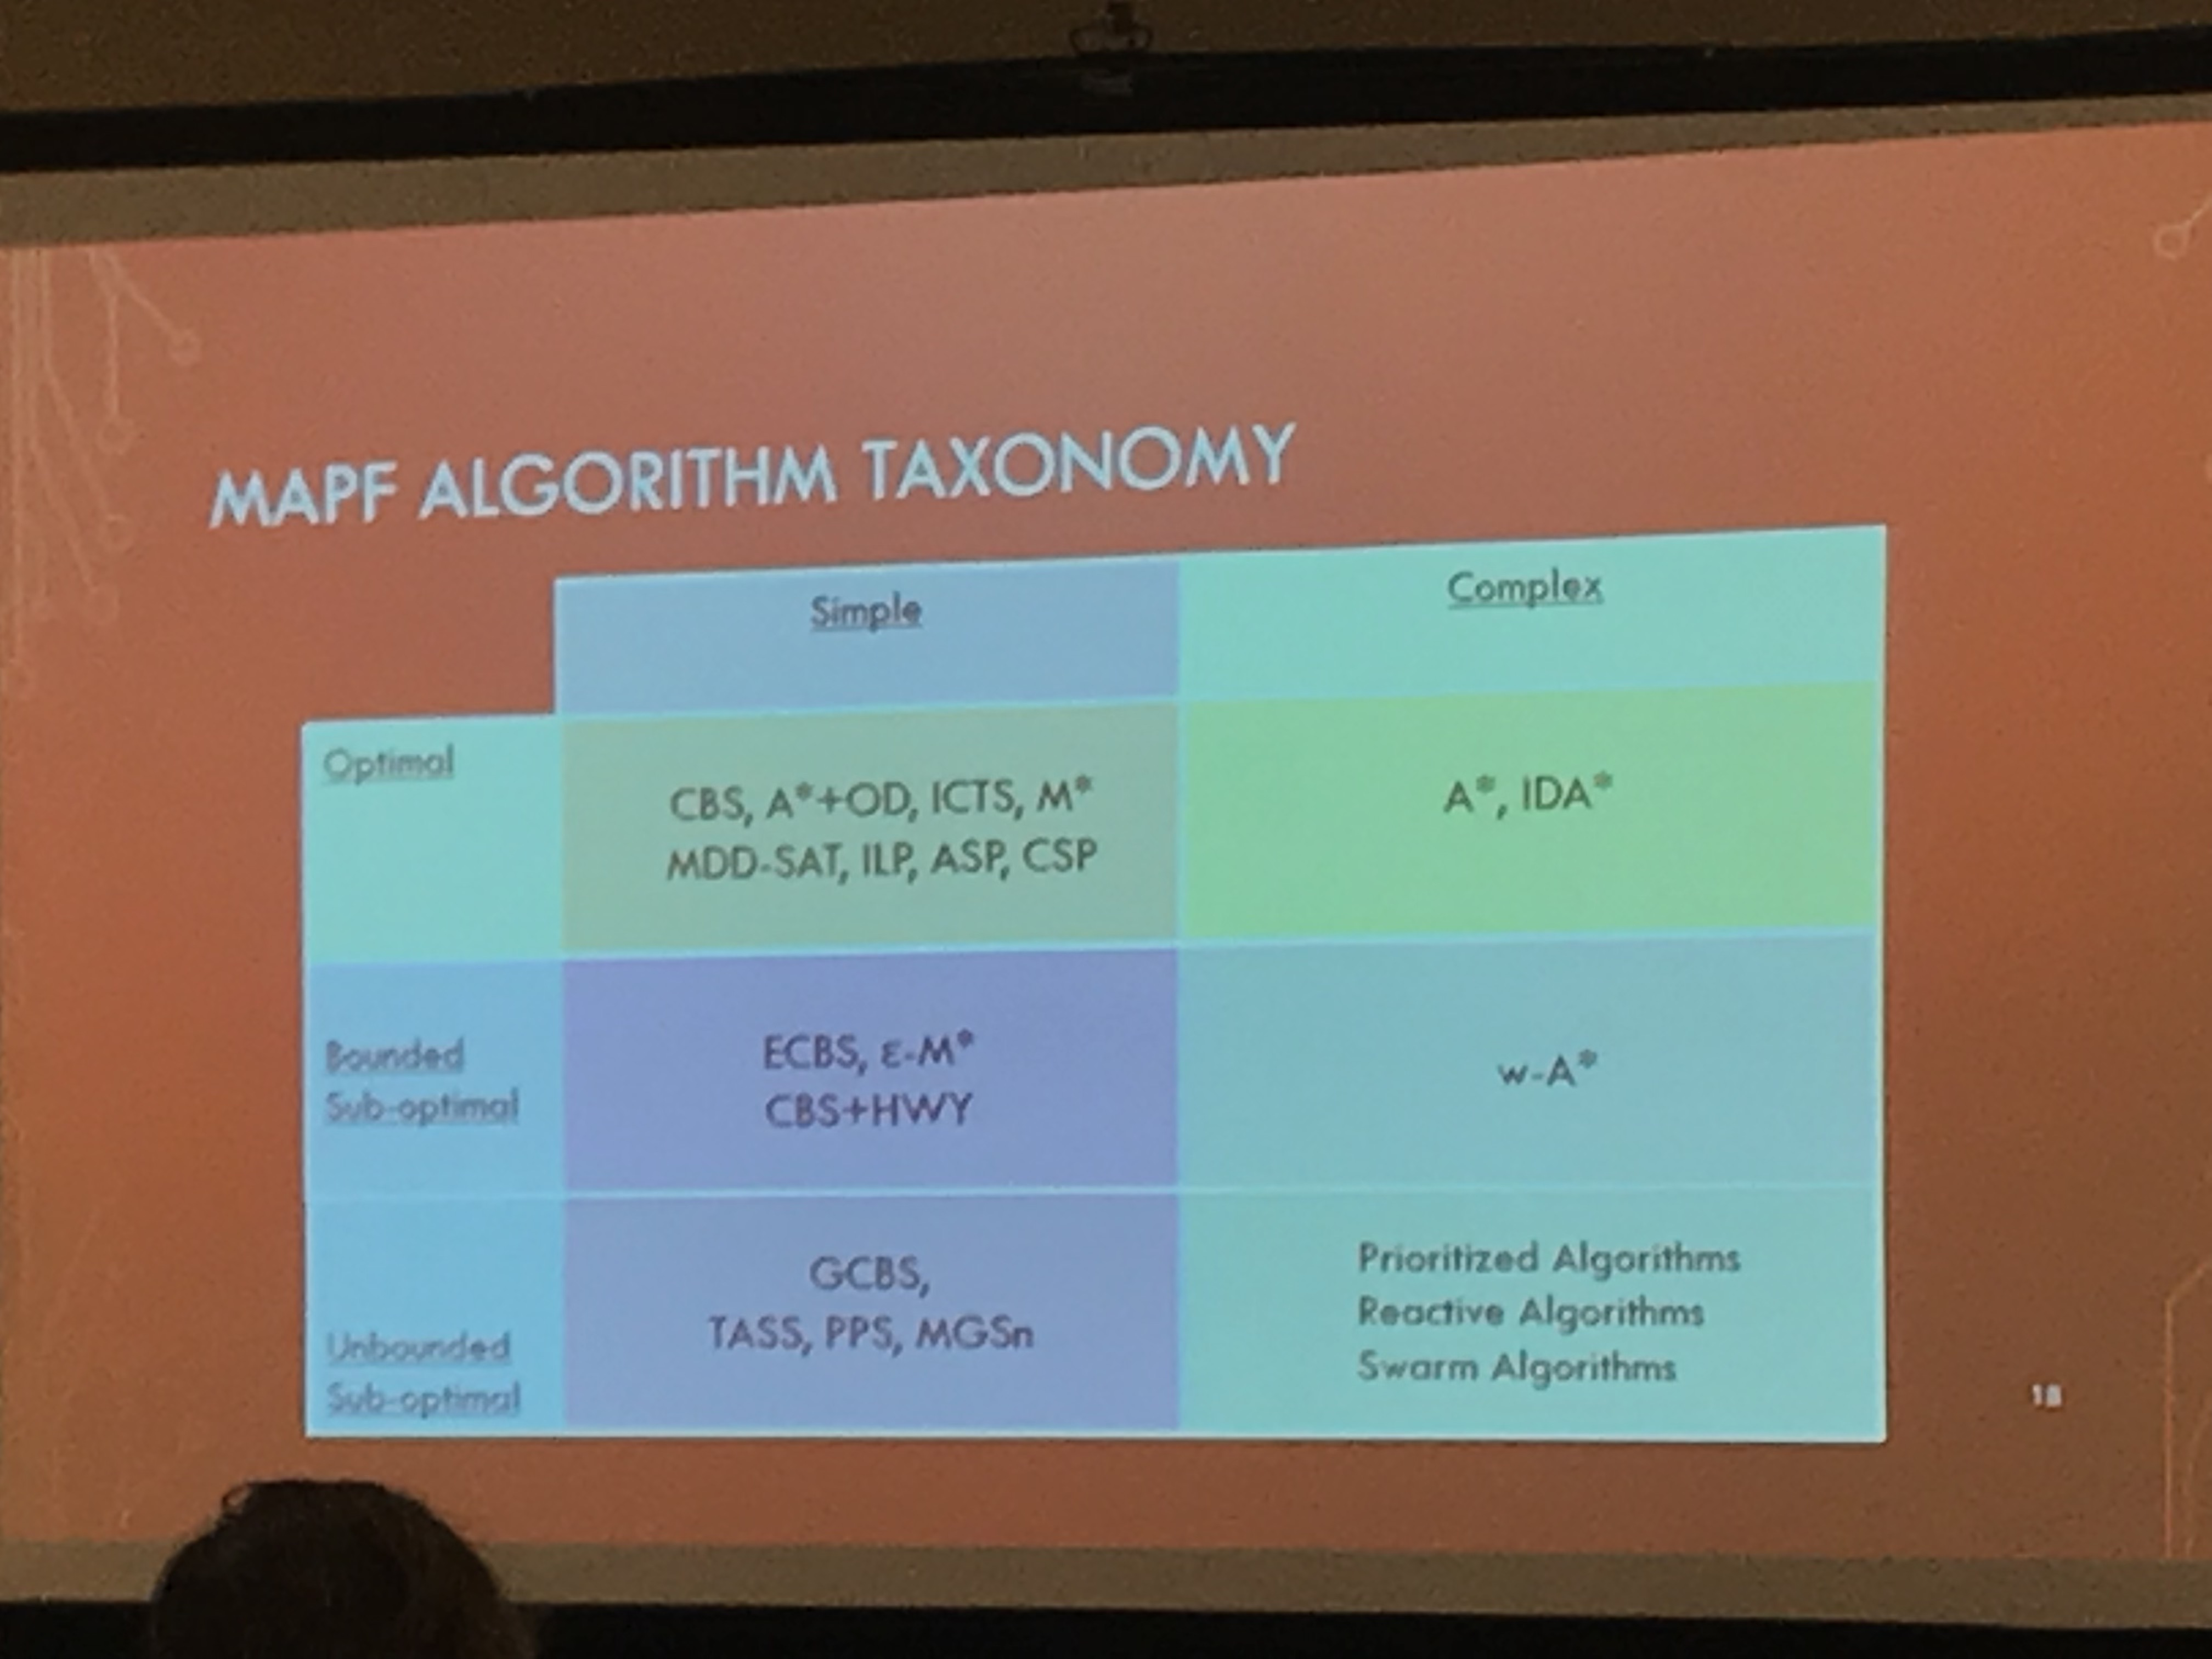
\includegraphics[width=0.5\textwidth]{images/mapf.JPG}
    \caption{Taxonomy of MAPF approaches}
    \label{fig:mapf}
\end{figure}

New approach 1: CBS + CL, which fills in the bottom right slot of Figure~\ref{fig:mapf}. \\

New approach 2: Extended ICTS, which extends the ``increasing cost tree search" algorithm for non-unit costs, which fits in the top right slot of Figure~\ref{fig:mapf}. \\

Current Work: extends conflict based search (CBS) CBS~\cite{sharon2012meta} by adding a conflict avoidance table and prioritization of conflicts. \\

Hypothesis: a particular statistic, ``ecap", can predict the effectiveness of approaches to conflict avoidance. ``ecap" means ``equivalent-cost alternate paths", which is roughly: $\frac{\text{num states in equivalent paths}}{\text{num states in optimal path}}$. \\

Extension: apply constraints over both time, overlaps of paths/edges, and other dimensions/planning constituents.

\spacerule
\subsection{Christopher Fourie: Adaptive Planning with Evidence Based Prediction}

Goal: robot needs to understand what a person is going to do in the context of a joint robot-person collaborative activity. \\

This involves: activity recognition, segmentation, and predictions. \\

Idea: we get less idle time with people/robot if robots can anticipate the person's behavior! So, let's get robots to anticipate behavior. \\

{\bf Research Goal:} Get collaborative systems to accommodate 1) individual behavioral patterns, 2) preferences in task ordering and timing, 3) new behaviors as they occur. \\

Focus: Repetitive Task Environments (RTEs). \\

{\bf Technical Approach:}
\begin{enumerate}
    \item {\it Modeling and an Activity Prediction Framework:} predicting activities in RTEs.
    \item {\it Planning for Improved Fluency:} in RTEs.
    \item {\it Human Experiments:} and the controlled evolution of fluency/efficiency in RTEs.
\end{enumerate}

Human-Study: collect data of people performing a partially ordered task as naturally as possible. Fit a gaussian model to the time taken by each person -- can then evaluate how well that model predicts the time taken for other people. \\

$\ra$ Finding: we're not sure if we can expect models like this to predict orderings and time taken for {\it new} people. Doesn't generalize all that well! Individuals are highly unique. But, inter-ordering behavior is consistent. \\

So, idea: define a temporal predictor for each ordering. Idea is to use a mixture model for predicting time-taken given the ordering (so its a mixture of orderings). \\

Next idea: learn an activity recognition model for sets of trajectories, and use this model to augment the temporal prediction.

\spacerule
% --- AI Roadmap ---
\subsection{AI Roadmap Panel}

To close out the night there will be a panel discussing the next 20 years of AI-research, chaired by Yolanda Gil and Bart Selman. \\

\begin{figure}[h!]
    \centering
    
\includegraphics[width=0.5\textwidth]{images/ai_roadmap.JPG}
    \caption{AI Roadmap}
    \label{fig:roadmap}
\end{figure}

US Congress said, in November: we do not want to legislate anytihng about AI/ethics/society, since we (meaning congress) don't understand AI (instead they should turn to researchers). \\

Research roadmap was commissioned by the NSF -- Computing Research Association (CRA) and Computing Community Consortium (CCC) are main institutions behind the roadmap. \\

Objectives:
\begin{itemize}
    \item 10-20 year Roadmap
    \item Guidance for funding agencies and congress.
    \item Relate to AI research in industry.
    \item International AI initiatives.
\end{itemize}

Other documents:
\begin{itemize}
    \item US National AI RandD strategic plan, 2016: \url{https://www.nitrd.gov/news/national_ai_rd_strategic_plan.aspx}
    \item US National Robotics Roadmap, 2006, revised 2006: \url{https://cra.org/ccc/wp-content/uploads/sites/2/2016/11/roadmap3-final-rs-1.pdf}
    \item 100 year study of AI, 2016 report: \url{https://ai100.stanford.edu/}
    \item AI strategies/investments abroad: \url{https://medium.com/politics-ai/an-overview-of-national-ai-strategies-2a70ec6edfd}
\end{itemize}

Held three workshops on 1) Integrated Intelligence, 2) Meaningful Interaction, and 3)

They'll next give summaries of each workshop and their objectives.

\subsubsection{Integrated Intelligence}

Marie Desjardins is the speaker. We thought about three big themes: 1) Mind, 2) Knowledge repositories, and 3) Contextualize AI. \\

{\bf Goal:} Be cross cutting, focus on big interdsciplinary areas that can have big impact. Identified four core areas:
\begin{enumerate}
    \item {\bf Science of integrated AI.} This is all about the {\it integration} of the many subfields we've studied thus far. How do we bring together perception, deliberation, and control? Metareasoning, reflection? What are the components of intelligence?
    \item {\bf Contextualized AI.} involves personalization, social cognition, persistent over time, highly customizable to individuals.
    \item {\bf Open Knowledge Repositories,} we {\it can't} have closed off knowledge bases for individual institutions. This needs to be a community resource! \dnote{Wow that's a fascinating idea.}
    \item {\bf Understanding Human Intelligence.} Unifying theories of human and artificial intelligence, AI to understand human intelligence, and AI inspired by human intelligence.
\end{enumerate}

\subsubsection{Meaningful Interaction}

The speaker is Dan Weld. This workshop focused on collaboration, trust and responsibility, diversity of interaction channels, improving inline interactions. \\

A few societal vignettes to concentrate on, including robot caregivers, training for robot repair jobs, custom personal devices, and so on.

Main technical areas:
\begin{enumerate}
    \item {\bf Collaboration:} how can we model human mental states, get AI systems to understand people better, reliability and ethical behaviors.
    \item {\bf Diversity of Interaction Channels:} diversity of human ability, multimodal explanations, privacy preservation across channels.
    \item {\bf Trust and Responsibility:} Transparency and explanation, debugging behaviors, boundaries and responsibility.
    \item {\bf Improving Interactions Between People:} customized presence, collaborative creation, reputation and factfulness.
\end{enumerate}

\subsubsection{Self-Aware Learning}

The speaker is Tom Dietterich. This workshop focused on robust and trustworthy learning. \\

Main technical areas:
\begin{enumerate}
    \item {\bf Robust and Trustworthy Learning:} Quantifying Uncertainty, identifying risks/failure modes, failing gracefully.
    \item {\bf Deeper Learning for Challenging Tasks:} learning from few examples, learning through interactions, long-term adaption.
    \item {\bf Integration of Symbolic and Numeric Representations:} abstracting symbols from numeric representations, explainable and instructable AI, representing complex structures beyond word embeddings.
    \item {\bf Learning in Integrated AI/Robotic Systems:} robust object manipulation, learning from humans by demonstration and instruction.
\end{enumerate}

\subsection{A New Era of Audacious AI Research}

Now Bart Selman is the speaker. ``Audacious" AI research tackles broader AI goals. Basically: how can we do massive scale AI projects? ({\it a la} the hubble, LHC, human genome project?) \\

Proposed Recommendations:
\begin{enumerate}
    \item {\bf Open National AI Platform:} shared ecosystem/infrastructure for AI research, example resources, data repositories, wide range of contributors, hardware/data/software/services.
    \item {\bf Broaden AI Education:} need for education of official degrees/certifications in AI at all levels, fellowships for grad students, need creative incentive mechanisms.
    \item {\bf Promote AI Policy and Ethics:} promote AI research that focuses on characterizing and quantifying AI systems, need to promote emerging cross-cutting disciplines for AI.
\end{enumerate}


\subsubsection{Q\& A}
Now onto some Q \& A! They also gave out an email address folks can contact with questions or ideas: \url{gil@isi.edu}, \url{selman@cs.cornell.edu}, and \url{cccinfo@cra.org} \\

Q: You mentioned some public resources (like data sets/hardware available for public use) -- who will build such a thing? \\

$\ra$ A: Well, we're mostly defining the agenda, and trying to highlight the landmarks that we can hit if we invest our resources as a society in the right way. \\

Q: If we build a communal knowledge graph, how do we do that in a way that is unbiased? Make it open? Targeted initiatives? \\

$\ra$ A: Yes! We discussed this point a lot. Social norms and counterfactuals and fictional worlds are all very challenging things to embed in a knowledge graph. There will absolutely not be the ``one true" perspective on the world. \\

Q: What's the plan for the roadmap given that governments around the world are realizing the power of AI and are starting to regulate AI? Might interfere with what we do/want to do? \\

$\ra$ A: We take the position that we support fundamental research in AI, and open research in AI. There's a military component that we do not really address. 

$\ra$ A2: many ways folks might want to control AI -- control for good of society, good of individual/country. We discuss control of intellectual property in the doc. Core philosophy: roadmap is how we open the development of AI techniques so we benefit all of society. \\

Q: Sharing info among AI researchers, as with arXiv. Some of the presentations from today were online, for instance. It's helpful to have shared presentations/papers. Any ideas for sharing work more easily? \\

$\ra$ A: That's an important insight! The more we understand each others' expertise/perspective the better. So let's continue to focus on open/accessible software/data/papers. \\

Q: How does modeling business processes show up in the roadmap? \\

$\ra$ A: Definitely came up in the workshop(s). \\

Q: How do companies/industry fit into the roadmap? I didn't see them show up all that much. \\

$\ra$ A: Many folks in industry are involved, lots of people at the workshops were from industry. Your point is well taken and we welcome involvement from industry. \\

\dnote{Now the Q\& A is moving to a more open ``suggestion/general question" session}

Q: A suggestion -- focus on natural disasters (see: Harvey, Katrina, wildfires). \\

Q: Lots of societal challenges on the horizon -- thoughts on how to tackle them? \\

$\ra$ A: well, we're trying to draw on many disciplines to better understand and prepare for this impact. \\

Q: This is really an international problem -- we're working on the same thing in Europe. So, perhaps we should connect our agendas. \\

$\ra$ A: Absolutely! We hope we can work on that soon. \\

Q (from Ed Feignenbaum!): To do what you laid out is going to take an {\it army} of AI research superstars. Half the trickle of people we train go off to Google/Microsoft/Facebook. Are you worried about this education problem? We need an army, we're getting a platoon! \\

$\ra$ A: Yes, this came up. We have to make academia an environment for doing this kind of audacious AI research. People find industry exciting because of the money, people, and research. Great question -- we'll raise this question in the report and will try our best to address this. \\

$\ra$ A2: we had a big discussion about this. Someone {\it during} the workshop got a 7 figure offer. No, we can't match that. But, maybe we can offer something else. \\

$\ra$ A3: Another thing we're addressing is how fast society can adapt to changes of all sorts. Also critical to ensure we can increase the diversity of CS education! \\

Q (CTO of lincoln labs): Aloha! Thanks for hosting this in Hawaii. Reminded of the early days of the internet/digital age: Optimism was huge, but later we found massive issues we didn't predict. My feedback is this: you have an opportunity/responsibility to put forward that perspective. It needs to be at the forefront. \\

Q: Curious about the definition of advancement of AI? What does it mean to progress AI? \\

$\ra$ A: We interpret intelligence very broadly -- human/biological/animal/artificial are all included. \\





Q: Lots of wonderful ideas for areas to focus on -- do you have suggestions for how to improve our research methods going forward, given the demands placed on us as a community?

%Q: Any thoughts on how we can change the incentive structures in the world to encourage the right kinds of work?

Q: So many of us probably saw Mark Zuckerberg explain really basic aspects of facebook and the internet to a panel of senators. My question is: how should we deal with the fact that policy makers will be forced to wrestle with areas they have no expertise in? What can we do to both work effectively with policy makers and make sure knowledgable people are involved in critical decision making?



% ------------
% -- Tuesday --
% ------------
\section{Tuesday January 29th}
The official conference sessions begin! We start with some opening remarks from the President of AAAI, Yolanda Gil. \\

New code of conduct available on the conference website\footnote{\url{https://aaai.org/Conferences/AAAI-19}}. \\

Now, the chairs: Pascal Van Hentenryck and Zhi-Hua Zhou. \\

First, we remember some people we lost this past year:
\begin{itemize}
    \item Alan C Schultz (1957-2019), Naval Research Laboratory. 
    \item Zohar Manna (1939-2018): wrote many books in AI, focus on temporal logic and automated theorem proving.
\end{itemize}

Acknowledgements:
\begin{itemize}
    \item Best Paper committee: Boi Falting, Fei Sha, \dnote{one other I missed :(}
    \item Eugene Freuder as Presentation Chair -- put a lot of work into improving the oral presentations.
    \item For priceless advice, Sheila McIlraith and Killian Weinberger (chairs from last year) and Yolanda Gil (president).
    \item Peng Zhao, workflow chair.
    \item The 89 AC, 322 SPC, and 3450 PC members.
    \item Amazing AAAI staff: Carol Hamilton, Monique Abed, Diane Mela, Ipshita Ghosh, Juliana Rios, Mike Hamilton, and Kapil Patnaik.
    \item Kevin Leyton-Brown and Milind Tambe for organizing the AI for Social Impact track.
\end{itemize}

{\bf What's new this year:}
\begin{itemize}
    \item Summary Reject procedure: if paper is not relevant to AAAI, violates blind submission policy/page limit, clearly too low quality, is plagiarizing. Very conservative! Ended up ``summary rejecting" 234 papers (out of $\approx$ 7,000, so only $3\%$.
    \item Bidding for papers: only chosen a smaller set for PC members to bid (150, ish).
    \item Used Toronto Paper Matching System and subject area to match reviewers.
    \item More strict double blind policy: SPC identity not visible to reviewrrs, AC identity is not visible to SPC and reviewers, reviewers did not no any identitifies.
    \item Added the following question to let SPC/AC judge how senior/junior the reviewer is.
    \item Presentation format selection: accepted papers had the opportunity to upload slides to determine if the paper would be well suited for an oral. SPC and AC make the recommendations. PC co-chairs finalize presentation format.
    \item 7,095 submissions. Most submissions ever! Quality was very high, though. Average scores were significantly higher than last year.
    $\ra$ AAAI will look for larger future venues to accommodate growth.
\end{itemize}

Now Zhiao will share somr statistics:
\begin{itemize}
    \item Abstract: 7745
    \item Full paper: 7095
    \item 18,191 reviews collected
    \item Over 95\% papers had at least 3 reviews
    \item Average 1250 characters for each review.
    \item Accepted 1147, 460 orals, 687 poster papers.
    \item 122 Technical Session
\end{itemize}

Some images to summarize:

\begin{figure}[h!]
    \centering
    \subfloat[]{\includegraphics[width=0.31\textwidth]{images/stats/stats_1.JPG}}
    \subfloat[]{\includegraphics[width=0.31\textwidth]{images/stats/stats_2.JPG}}
    \subfloat[]{\includegraphics[width=0.31\textwidth]{images/stats/stats_3.JPG}} \\
    %\subfloat[]{\includegraphics[width=0.31\textwidth]{images/stats/stats_4.JPG}}
    %\subfloat[]{\includegraphics[width=0.31\textwidth]{images/stats/stats_5.JPG}}
    %\subfloat[]{\includegraphics[width=0.31\textwidth]{images/stats/stats_6.JPG}}
    \caption{Stats on AAAI}
    \label{fig:aaai_stats}
\end{figure}


Next up, a quick summary of IAAI: huge diversity of application areas! 5 deployed application awards focusing on programming, life insurance. Milind Tambe won the ``Robert S. Engelmore Memorial Award". \\

{\bf Awards:}
\begin{itemize}
    \item Senior Member Presentation Track, chaired by David Aha and Judy goldsmith.

    $\ra$ Blue Sky Idea Track: 30 submissions, 15 accepted. 4 winners:
    
        \begin{enumerate}
        \item Explainable Normative and Justified Agency by Pat LAgley
        \item Building Ethically Bounded Agents by Francesca Rossi
        \item Recommender Systems: A Healthy Obsession by Barry Smyth
        \end{enumerate}
    
\end{itemize}

{\bf Awards:}
\begin{itemize}
\item New Fellows: Vince Conitzer, Luc De Raedt, Kirsten Grauman, Charles Isbell, Jiebo Luo, Huan Liu, Peter Stuckey.
\item Senior Members: Bo An, Roman Bartak, Yiling Chen, Cristina Conati, Minh Do, Eric Eaton, Vincent Ng, Marco Valtorta, Yevgeniy Varbeychik, and Kiri Wagstaff.

\item Classic Paper Award: Contend-Boosted Collaborative Filtering for Improved Recommendations: ``Content Boosed Collaborative Filtering for Improved Recommendations" by Prem Melville, Raymond J. Mooney, and Ramadass Nagarajan, presented at AAAI 2002: ``For showing a way to cmopletement content-based and collaborative filtering approaches in recomenndation systems.""

\item Classic Paper Honorable Mentiond: $D*$-Lite by Sven Koenig and Maxim Likhachev, also at AAAI 2002, ``For developing an incremental heuristic search algorithm for robot navigation in unknown terrain that is easy ot udnerstand analyze and extend."

\item Distinguished Service Award: Shlomo Zilberstein, ``For his sutained and conscientious service and leadership both to AAAI as a councilor and conference committee chair and to the broader AI community, as the president of ICAPS."

\item Feigenbaum Prize: Stuart Russell: "In recognition of high-impact contributions to the field of AI through innovation and achievement in probabilistic knowledge representation, reasoning, and learning."

\item AAAI/EAAI Outstanding Educator Award: Ashok Goel.
\end{itemize}


\spacerule
\subsection{Invited Talk: Cynthia Brazeal on Living and Flourishing with AI}

%Charles (as Michael Littman!) is introducing. \\

To start, consider: many of our world leaders {\it don't understand AI}. So, we have a grand challenge to work hard toward a positive future despite this fact. \\

We all know AI is transforming the workplace, but recently it's started to transform our personal lives too. See: amazon echo, home robots, drones, siri, and so on. Children today are growing up in a world where they can interact with AI. \\

Great products are not only useful, but the {\it experience} of them need to be emotionally uplifting and offer enhancement to the human experience. \\

\dbox{{\bf Main Question:} Can AI help us flourish?}

$\ra$ Relational AI (``relationship", not predicate/relation): AI that understands and treats people as people. We need:
\begin{enumerate}
    \item Emotional engagement.
    \item Collaboration between humans and AI as allies
    \item Personal relationships. \\
\end{enumerate}

To do this, we need to think of AI in terms of {\it socio-emotive} 1) perception, 2) learning, 3) interaction, and 4) expression. \\

Next set of transformative products and services will come from the intersection between AI and Design. Right now, these two fields are not deeply intertwined. We should be thinking about how to bring these two things together.

{\bf Main Goal:} Bring together these two fields. Today we'll see work in Social Robots and social/emotional intelligence in AI. \\

Cars? Baxters? These are (or will be) social in some capacity. Using gazes and gestures. \\

{\bf Three Key Themes}:
\begin{enumerate}
    \item Human Engagement.
    \item Allied Engagement, Personalization, and Learning.
    \item Aging: Fostering Community.

\end{enumerate}

\subsubsection{Human Engagement}

We have tons of processing power of our brain set aside for social processing -- so, we {\it need} AIs in our community to do the same. \\

We are a species that evolved to be in the physical co-presence of others, and we've found that the more our machines/robots embody these characteristics precisely because it's how our brain works. \\

To see this, let's look at some chat systems like Alexa. \\

Experiment: three different AI chat systems answering the question ``tell me about yourself".
\begin{itemize}
    \item Alexa:  I'm alexa, I can tell you the weather, etc.
    \item Jibo: My favorite things to do are talking to people and dancing. I also like Abe Lincoln.
    \item Google: I'm your google assistant, we can play mad libs, or spin the wheel.
\end{itemize}

``Robot Speed Dating" where families are brought into lab to interact with 3 different VUI agents. They ask questions to the three and then the people offer a diagnostic of the personality of these systems. \\

Takeaways: 1) people spend most of their time with these systems on social interactions, 2) the more ``personality" in the system, the more engaging people find them. \\

{\bf Thesis:} We are so profoundly social, so we have to pay attention to social aspects of these systems. \\

Q: What should the social dynamics of these systems be? \\

A: Can draw inspiration from human social interactions. It's dynamic, we need to form trust, and so on. \\

Three broad categories: 1) Intrapersonal context (smile detection), 2) Interpersonal context (trust), and 3) Intentional context (story telling). \\

Experiment with two children reading a story together. Basically: we want to model emotional understanding as intentional inference. Take a Bayesian theory of mind -- storyteller views it as a planning problem, uses social cues to monitor listeners understanding (POMDP). \\

\subsubsection{Allied Engagement, Personalization, and Learning}

Bloom 2 sigma effect: prek-12 US education, not ready to learn, can't catch up. 60\% children don't attend preschool. 37\% of 12th graders read at or above proficient level. \\

Different designing a tutoring system for kids vs. adults. Kids learn through play and interaction! \\

$\ra$ So, main focus has been on developing a robot for teaching kids through play and social interaction. Treat Robots as peer-like learning companions. \\

Big Finding: social influence and emotion. If a kid plays a math game with a robot where the robot says ``your brain grows the more you try!" it nurtures a {\it growth} mindset. Basically kids want to emulate the robot if they feel raport with the robot. \\

Q: What Role should a peer-like learning companion take and when? \\

A: Explored this question with a robot helping kids learn vocabulary (robot video!). Robot has different roles: could be a tutor or tutee. Different behaviors depending on whose ``turn" it is. Robot can offer explanation, give definitions, correct demonstrations as a tutor. As a tutee, the robot can ask for help, ask for explanation, show curiosity and growth mindset. The kid said ``I believe in you!" to the robot.\\
\dnote{This video was powerful! Really gives a hint of an incredible vision of the future} \\

Used RL in this setting. Have actually applied this system to schools in diverse Boston public schools. \\

Finding: Actual students learn better when the robot plays the adaptive role (both tutor/tutee) than the other cases. \\

Recent work on storytelling~\cite{park2017telling}, new paper at AAAI this year. \\

Q: How can we foster a positive relationship between kids and robot tutors/peers? \\

A: See recent work!~\cite{westlund2018measuring}.


\subsubsection{Aging: Fostering Community Connection}

We live in a ``silver tsunami" -- we can't train enough people or build enough facilities to help elders. \\

Q: So, how can we use robots and AI to help with elder care? And so in a way with respect and dignity? \\

Main struggles of elderly: lonelieness, helplessness, boredom. \\

One route explored: use Jibo the robot to bring some joy to elders. It can dance, play the radio, take photos, tell jokes, and talk with folks. Designed to be a smart pet that can help with things -- people that might usually be intimidated by technology readily engage and have fun with Jibo. \\

$\ra$ So, explored social robots for bringing joy to people. Older adults are the {\it most open} to these technologies. Huge positive response, they want to embrace these technologies. \\

Research Q: Can a social robot foster human-human connection in communities? (not just human-robot) \\

A: Yes! This really works. The social robot becomes a catalyst for people to be more openly social and form deeper social connections among each other. \\

$\ra$ huge opportunity for humanistic and social design to make an impact in peoples lives! \\

{\bf Takeaway:} Social engagement isn't just about making it fun. \\

Would love to see the community focus on:
\begin{itemize}
    \item Human factors and long term interactions between people/robots.It's hard but we need to do it!
    \item Ethics: educate people/next generation (including elementary school!), design appropriately, democratize AI -- need AI to close the prosperity gap, not enhance it.
\end{itemize}

To close: a video of (young!) kids playing with Scratch -- they're in early elementary school. And the amazing thing is, the right tools (Scratch) can actually give kids the opportunity to learn about the ideas in ML/AI/CS. \\

Punchline: ``in a world of intelligent machines, humanity is the killer app" -- it is so important that we design these systems to be {\bf human centered}.


\dnote{I have meetings now, will check back in for Learning theory in the afternoon}

\spacerule
\subsection{Learning Theory}

Now for some learning Theory!

\subsubsection{Precision-Recall vs. Accuracy~\cite{juba2017precision}}

Paper by Brendad Juba and Hai Le. \\

\ddef{Class Imbalance}{One (or a few) classes severely out-represent other classes in some dataset.}

So, pracitioniers find classification harder for imbalanced data, but learning theories suggest that imbalance shouldn't matter. \\

{\bf Goal:} Analyze disconnect between learning theoretic view of data imbalance and practice. \\

Idea: need a new metric. Namely, learning theory usually suggests the use of {\it accuracy}, but we really need high precision or recall. \\

Case Study: Machine Translation -- we find that 10s of billions of examples increases accuracy. But, why? Why does it need so much data? \\

{\bf Main contribution:} derive relationship between precision-recall \& accuracy. \\

$\ra$ Takeaway: Large data set is the cure for data imbalance. \\

Main theorem:
\begin{theorem}
Suppose $D$ is a distr over examples with boolean labels with a base psotive rate of $\mu \Pr_D(c = 1)$, $h$ is a weak learner, and $\eps_{prec}, \eps_{rec}$ and $\eps_{acc}$ are the precision, recall, and accuracy error for $h$ on $D$. Then:
\[
\eps_{max} = \max[\eps_{prec},\eps_{rec}],
\]
satisfies:
\[
\mu \eps_{max} \leq \eps_{acc} \leq \mu\left(\eps_{rec} + \frac{1}{1 - \eps_{prec}} \eps_{prec}\right)
\]
\end{theorem}

Conducted experiments comparing performance of different techniques for fixing class imbalance. \\
Observations:
\begin{itemize}
    \item Training on  a large data set improve precision and recall of class imbalance problem,
    \item Can't rely on preprocessing to fix this.
    \item Hard to achieve high precision-recall under severe class imbalance unless one possess a large amount of training data.
    \item Methods for correcting class imbalance don't often help.
    \item {\bf Advice:} Incorporate explicit prior knowledge about the domain.
\end{itemize}


\subsubsection{Theoretical Analysis of Label Distribution Learning}

Paper by Jing Wang and Xin Geng. \\

\ddef{Label Distribution Learning (LDL)}{Learning setting wherein each label $y$ is related with the instance $x$ with label description $d_x^y$. \\

Basically: feature space $X \in \mathbb{R}^d$, label space, label distribution function $\eta : X \times Y \ra \mathbb{R}$. Training set $S = \{(x_1, d_{x_1}^{y_1} \ldots d_{x_1}^{y_n} \ldots )\}$. Learn a function from $x$ to $y$ given only these descriptions.}

Model: one hidden layer and multi-output neural network with softmax output function, sum-squared loss. \\


Main theorem bounds the Rademacher complexity of AA-B and SA-ME (two different learning algorithms for the LDL problem), which can then be used to bound the (generalization?) error:
\begin{theorem}
Upper and lower bounds on the Rademacher complexity of AA-BP: for a loss function $\ell$ with Lipschitz constant $L_\ell$;
\[
\square \leq \mc{R}(\ell \ldots ) \leq \square
\]
\dnote{The bounds were complex, see the paper for details!}
\end{theorem}


\subsubsection{Dynamic Learning of Sequential Choice Bandit Problems}

Paper by Junyu Cao and Wei Sun. \\

Example: you probably have received app notifcations/emails from apps you use. Positive: might boost engagement rate, but Negative: lead to marketing fatique and cause disengagement. \\


{\bf Goal:} How can we address this trade-off? Questions: can we,
\begin{itemize}
    \item Determine optimal sequence of messages?
    \item Dynamically learn users preference/patience?
\end{itemize}

Problem setup: $N$ different messages to choose from. Each message $i$ generates revenue $r_i$ when selected by a user. For a user arriving at time $t$, the platform determines a sequence of messages $\bm{S} = S_i \oplus S_{i+1} \ldots$. \\

User's choice: a user can either accept or reject a message. \\

Abandonment Distribution: Assume the probability a user abandons can be modeled as a geometric distribution. So: sequential choice model under marketing fatigue. User's valuation of a message denoted $u_i \in [0,1]$. \\

Get an expected utility optimization problem (optimizing over choice of sequence of messages). So:
\begin{equation}
    \max_S \bE[U(S)]
\end{equation}

Study both the online and offline variant.  Contribution:
\begin{itemize}
    \item {\bf Offline:} Come up with an efficient $O(N\log N)$ offline algorithm.
    $\ra$ Prove more patient customers will bring higher payoff.
    \item {\bf Online:} Present a Upper Confidence Bound (UCB) like approach for the online SC-Bandit setting. Analyze this regret, which comes out to:
    \[
    \text{Regret}(T,u,q) = O(N \sqrt{T \log T}),
    \]
    where $T$ is the horizon, $u$ is the valuation, \dnote{missed $q$}.
\end{itemize}

Further {\it personalize} to individual users using Contextual SC-Bandits. Adopt the generalized linear bandit framework to do similar UCB like updates in the contextual setting. \\

Experiments in both the traditional SC-Bandit and the contextual SC-Bandit. 

\subsubsection{Near-Neighbor Methods in Random Preference Completion~\cite{liu2019nearneighbor}}

Paper by Ao Liu, Qiong Wu, Zhengming Lu \\

Consider recommender systems. Data are normally 1/5 stars, etc. But, in more generaly systems, we might imagine ranked preferences, or pairwise rankings. \\

Q: Can we use near-neighbor methods for doing random preference completiong? \\

Setting: $y_1 \ldots y_m$ alternatives, and $x_1, \ldots, x_n$ agents with given preferences over the alternatives. \\

More formally: KT-kNN algorithm, based on:
\[
NK(R_i, R_j) =\frac{\text{\# Pairs ranked opposite in $R_i, R_j$}}{\text{\# Pairs ranked both by $R_i$ and $R_j$}}
\]

Can then use $NK$ between all agents to find nearest neighbors. \\

Q: Is $NK$ an effective metric for doing nearest neighbors in this context? \\

A: Yes! See~\citet{katz2017nonparametric}.\\

{\bf Open Question:} Algorithms work under deterministic setting usually also work under random settings. Why? \\

Main Result 1 shows the predicted nearest neighbor by KT-kNN is far off from the desired prediction under a particular noise model (Plackett-Luce noise):
\begin{theorem}
For $1D$ latent space with at least .5 probability:
\[
||x_{KT-kNN} - x^*|| = \Theta(1),
\]
with $x^*$ the ``desired" prediction.
\end{theorem}

So, given this result: can we overcome this difficulty? \\

A: Yes! Through Main Result 2 $\ra$ Anchor-kNN. \\

Anchor-kNN uses information from other agents' rankings. We now get features characterizing other agent's choices. Then:
\begin{theorem}
For $1D$ latent space with at least .5 probability, if all agents rank at least poly-log(m) alternatives, with probability $1-o(n^{-2})$:
\[
||x_{Anchor-kNN} - x^*|| < o(1),
\]
with $x^*$ the ``desired" prediction.
\end{theorem}

Further conduct some numerical experiments to validate anchor-kNN relative to the KT-kNN. Takeaway: no matter what metric they tested with, they got great performance with Anchor-kNN. Further evaluate on a real dataset (Netflix) and find a huge improvement \\

Conjecture: their theorems generalize to higher dimensional spaces (instead of just 1D). \\

\subsubsection{Dimension Free Error Bounds from Random Projections~\cite{kaban2019dimension}}

Paper by Ata Kaban. \\

{\bf Research Question:} What makes some high dimensional learning problems easier than others? \\

Background: Learning from high dimensional data is challenging. Generalization error depends on input dimension in an essential way. How can we get a more flexible/available notion of generalization error? \\

Notation is typicl: $\ell \mc{Y} \times \mc{Y} \ra [0,1]$, $\mc{H}_d : \mc{X}_d \ra \mc{Y}$ is the hypothesis class, training set, $\bE[g]$ will mean generalization error, $\bE[\hat{g}]$ will mean training error. \\

{\bf Main Idea:} Translate some high dimensional data via a random project to make learning easier. \\

\ddef{Compressive Distortion}{Take $R \in \mathbb{R}^{k\times d}$ to be a random matrix full rank. Apply $R$ to all input points. \\

Consider an {\it auxiliary function class} $\mc{G}_R = \ell \circ \mc{H}_d$.\\

The compressive distortion of a function $g \in \mc{G}_d$ relative to $g_R \in \mc{G}_R$ is the following:
\[
D_R(g,g_R) = [g_R \circ R - g]
\]
}
Has some nice be properties: bounded independently of target if loss is Lipschitz, 0 if $k$ is sufficiently large, choice of $k$ is up to us. \\

Can then define a new complexity measure:
\ddef{Data complexity}{Of a function class $\mc{G}_d$ is given by:
\[
C_{2N,k}(\mc{G}_d) = \bE \sup_{g \in \mc{G}_d} \inf_{g_R \in \mc{G}_k} D_R(g,g_R)
\]
}

Main theorem:
\begin{theorem}
For any $\delta > 0$, w/ Pr $1-2\delta$ unfiromly for all $g \in \mc{G}_d$:
\begin{equation}
    \bE[g] \leq\hat{\bE}[g] + 2C_{2N,k}(\mc{G}_d) + \underbrace{\ldots}_{\text{Rademacher term}}
\end{equation}
\end{theorem}
Applications: can reduce or eliminate dimensional dependence of generalization guarantees for a variety of domains. \\

\dnote{I have meetings the rest of the day until the debate!}

\spacerule
\subsection{Oxford Style AI Debate}

\dbox{{\bf Proposition:} ``The AI community today should continue to focus mostly on ML methods."} \\

The debaters:
\begin{itemize}
    \item Team one (AGAINST): Oren Etzioni (OE), Michael Littman (ML)
    \item Team two (FOR): Jennifer Neville (JN), Peter Stone (PS)
\end{itemize}

Kevin Leyton-Brown (KLB) is moderating. \\

\subsubsection{Opening Statements}

JN: Let's start by talking about the goals of AI research. Goal is to understand the nature and limitations of computational intelligence. We also aim to create robust autonomous agents that can behave rationally and intelligently. Point 1: history of AI! 1956 Summer at Dartmouth they thought they could {\it solve} computer vision (in a summer). Reason being: unlike many other AI problems, vision is tractable and easy to encode. Rough timeline:
AI Winter in the 70s. Things turned around in 80s and 90s, like IBM used statistical models for translation. Then we started using big data sets for learning, Tesauro made TD-Gammon in the 90s, 2006 Netflix competition to develop an ML technique for reducing prediction error (Netflix says 75\% of things watched are from reccomendations). Hinton's group in 2012 used CNNs on ImageNet to great success, AlphaGo in 2016. All these breakthroughs were all due to machine learning. Therefore, we should continue focusing on ML b/c that's where our progress came from. \\

OE: Last five years have seen populist movements. 1) The Donald in the USA, 2) BREXIT, 3) a populist movement toward machine learning. You might ask: what's wrong with ML? We're hip! We get good results. I worry about an AI winter. Populist movements are all fine, they get 10\% gains on things b/c of CNNs, RNNs, ABC, HBO, etc. But, what happens when this continues? Let's look at the key people in these movements: Roger Stone dresses like Hannibal Lecter and was arrested by FBI agents that volunteered to arrest him. The machine learning movement has Peter Stone! No coincidence there? ML populist movement is plotting. They're trying to BUILD A WALL between ML and AI! We know better. Let's get a little more serious and dispense with some obvious points. ML has been successful: deep learning has exceeded expectations! Let's define ML, though. Our adversary may attempt to redefine ML in many serious ways. ML is ML (is ML) -- it's supervised learning (with a cherry on top!). In reality, ML is limited: people choose the architecture, data, regularization, loss function, and so on. It takes blood sweat and tears to get it to work. ML is 99\% human engineering/art. But the ML populist movement is claiming a lot more! AlphaGo -- what about MCTS?

KLB: thanks for those great remarks on Brexit and some AI. \\

PS: What you're asked to judge is not how deep our voice is, or how funny we are -- the question is whether we should continue focusing on ML in AI. And we should! For two reasons 1) it's our weakest link, and 2) we have the resources/people to make rapid progress. Focusing on ML now is healthy for our field. Many successes in AI -- {\bf decades} spent on symbolic reasoning. We then recognized it would be possible that it is impossible to solve perception perfectly. We're now in a phase of focused attention on understanding the degree to which ML can recognize and understand the world. This is very healthy! We're not taking a position on whether ML is more important. Just that we should focus on it now. Now is the moment for ML in the field! 60\% of papers at AAAI were on ML/NLP. What will this focus provide? We may be able to answer some of our central questions like how to scale with human interaction, transfer learning, one shot learning and so on. Lots of energy -- let's not throw it away. To summarize: we should keep focusing on ML b/c 1) it's our weakest link and we don't yet know the limitations, and 2) we have the critical mass to make serious progress. \\

ML: Nothing against ML! My initials. That being said, Peter would have the rest of AI be left alive in small dedicated communities. That's worrisome! 60\% of papers in ML related disciplines? What about the change over time! This trend might actually be problematic. We had the easier side to argue partly because there's a lot of ways to tackle the problem of creating intelligence. So, our side is right if literally anything else makes progress. Something ML is doing right is {\it redefining problems to be well suited doing ML}. I made the case to Peter Norvig that we should use more structure in robotics -- we don't see people solving problems in cross word solving. This would be a total mess to do deep learning! To me, ML systems are really attacking a different part of cognition than other parts of AI. It's sort of system 1 and 2 from Kahenmann and Tversky -- ML is system 1. System 2 is reflection/structure/consistency. We need System 2. No long term coherence. Example (because y'know, puns): pun generation. Punning riddle: what do you call a green cow in a field? Invisibull! A deep learning system was trained on puns then generated: What do you call a short sense of humor? A charming saucer! It sounds like a joke, but all the depth/meaning/structure is missing. It's very surfacey. Alternatively, using GOFAI, same thing: what do you call a murder that has fiber, a cereal killer. And that was better! so, QED. \\

KLB: Transition to free-for-all stage. Respond to things people made. \\

OE: Peter Stone and I definitely agree -- just like Roger Stone, Peter has a perception problem. At 9000 problem there were people at AAAI! Biggest point to make: we don't want to throw it away. We want to note that it's a tool, not a panacea. \\

PS: Thank you Oren for reiterating my point exactly! It's a tool in the toolbox, and one we know the least about so far. Would also like to respond to Oren -- we need to keep other communities alive. Continue our focus now on ML. Michael's thesis, was also quite good, algorithms for sequential decision making using machine learning! Yes Peter Norvig should be here. Yes my name is Stone. \\

JN: Michael said he was dissappointed in Peter and I for originally being ML people that worked in complex structure problems that now we do learning -- deep learning just worked better when I applied it! Also, when we say machine learning we do {\it not} meen deep learning. We mean all of machine learning. It's a big umbrella! As a community, we start off by asking if problems are intractable. We've gotten to larger and larger problems over time because of machine learning. Like MCTS was able to be successful in AlphaGo because of learning! \\

KLB: AAAI chairs pointed out that most papers submitted come from ML but most folks in the crowd said no! \\

OE: It's simple! If you're thinking in the short term, like publishing, it's a way to publish. Yesterday in the road map session the question was raised ``how do we build a general theory of intelligence". It's one of the most profound scientific questions we can ask. We're going to need a lot more than gradient descent. \\

ML: It's important to do ML in the context of structures/human in the loop. \\

OE: I'd like to clarify. The proposition is about it being {\it mostly} ML. We're not about it being zero ML. Let's not bargain over the price, let's think about the fundamental questions. The debate is about cognitive architecture. What's more complex? Intelligence or chrome browser? Chrome has 7 million lines of code. Are we really going to learn 7 million lines of code? We need structure. Mostly ML ain't going to cut it. \\

PS: We're not disagreeing about the larger picture. We want a general theory of intelligence. Our big question is to understand the nature and limits of computational intelligence. And yes in the long run we take a big tent view: all areas are important. But, we already know what to do when we have symbols. We don't know how to get the right symbols, we don't know the limits of ML. We should focus on ML until we identify their limits.\\

JN: I'd like to go back to McCarthy's statement at the Dartmouth Summer Conference -- ``every aspect of learning or other feature of intelligence". Just want to point out: first thing he points out is learning. Our focus on ML was at the core of AI as described to begin with. \\

KLB: Closing statements. \\

ML: So this was interesting! I kind of signed up to be on the other side when the proposition was different. I don't know if I buy Peter's story about ``do ML now" and then ``do other stuff later". The statement is sort of about focusing on ML indefinitely.. Anyway. I've been working with lots of scientists that want to skip the hard computation and get to something that just works quickly, which brings them to deep learning. I really do worry about these systems not having internal consistency. Machine generated music is not music -- it's nonsense. Worried about the fact that we redefine the problems so that we can generate slightly better nonsense. Ultimately ML is definitely integrated into the bigger picture. We need to think about how to integrate symbolic/deep. In fact we need to think about how symbolic approaches might need to change in light of recent advances in learning. \\

PS: It's clear that this statement is true. At our current state of knowledge in the field, ML is our weakest link, and we have lots of energy focused on it now. So we should capitalize on that to put a lid on those questions, now is the moment for ML. \\

OE: Kevin let's not get personal here that's my job. My worthy adversaries in no way address my comments about Trump or Brexit. Since our so called moderator accused our side of lacking substance, here we go: we're in the midst of a revolution, certainly. But we need to go beyond classifiers and think about the deep issues we face. These require synthesis with other approaches and caring about different problems like using common sense to avoid brittleness, choosing what to learn in the first place. Newell and Simon studied cognitive architecture in the 80s! We drifted away from these problems. We can study these problems now with ML, but we can't just do ML. \\

JN: As a panel we got together and decised we were all pragmatists and that we care deeply about solving real world problems. So, we all care about including ML methods with a host of other techniques that come from other aspects of AI (planning, expert systems, reasoning on open worlds), so I don't think as a community we shouldn't focus on function approximation as a solution to all of these problems. I do agree with Oren's point (somewhere in his Brexit rant) that ML uniquly designs tasks so that their methods work well. Instead of finding tasks we can solve we need to find tasks that need solving. So in that sense, I'm arguing a bit for the other side. \\

KLB: Thanks! That was fun!\\

\spacerule



% ---------------
% -- Wednesday --
% ---------------
\section{Wednesday January 30th}
Onto Wednesday! Today starts with a keynote by Ian Goodfellow. \\

\subsection{Invited Talk: Ian Goodfellow on Adversarial Learning}

Topic: Adversarial ML! And how it relates to other topics. \\

Traditional ML: based on optimization -- choose a cost function $J(\theta_1,\theta_2)$, find $\theta_1$ and $\theta_2$ that minimize $J$. This works great for classifiers! We can gradually minimize $J$ through various techniques until we find the right parameters. \\

But: lots of other parameters we can't really optimize. \\

$\ra$ Let's instead fall back to game theory. Two players play a game -- player 1 wants to minimize the score of the game, player 2 wants to maximize. If it converges, we find an equilibrium point.\\

\begin{figure}
    \centering
    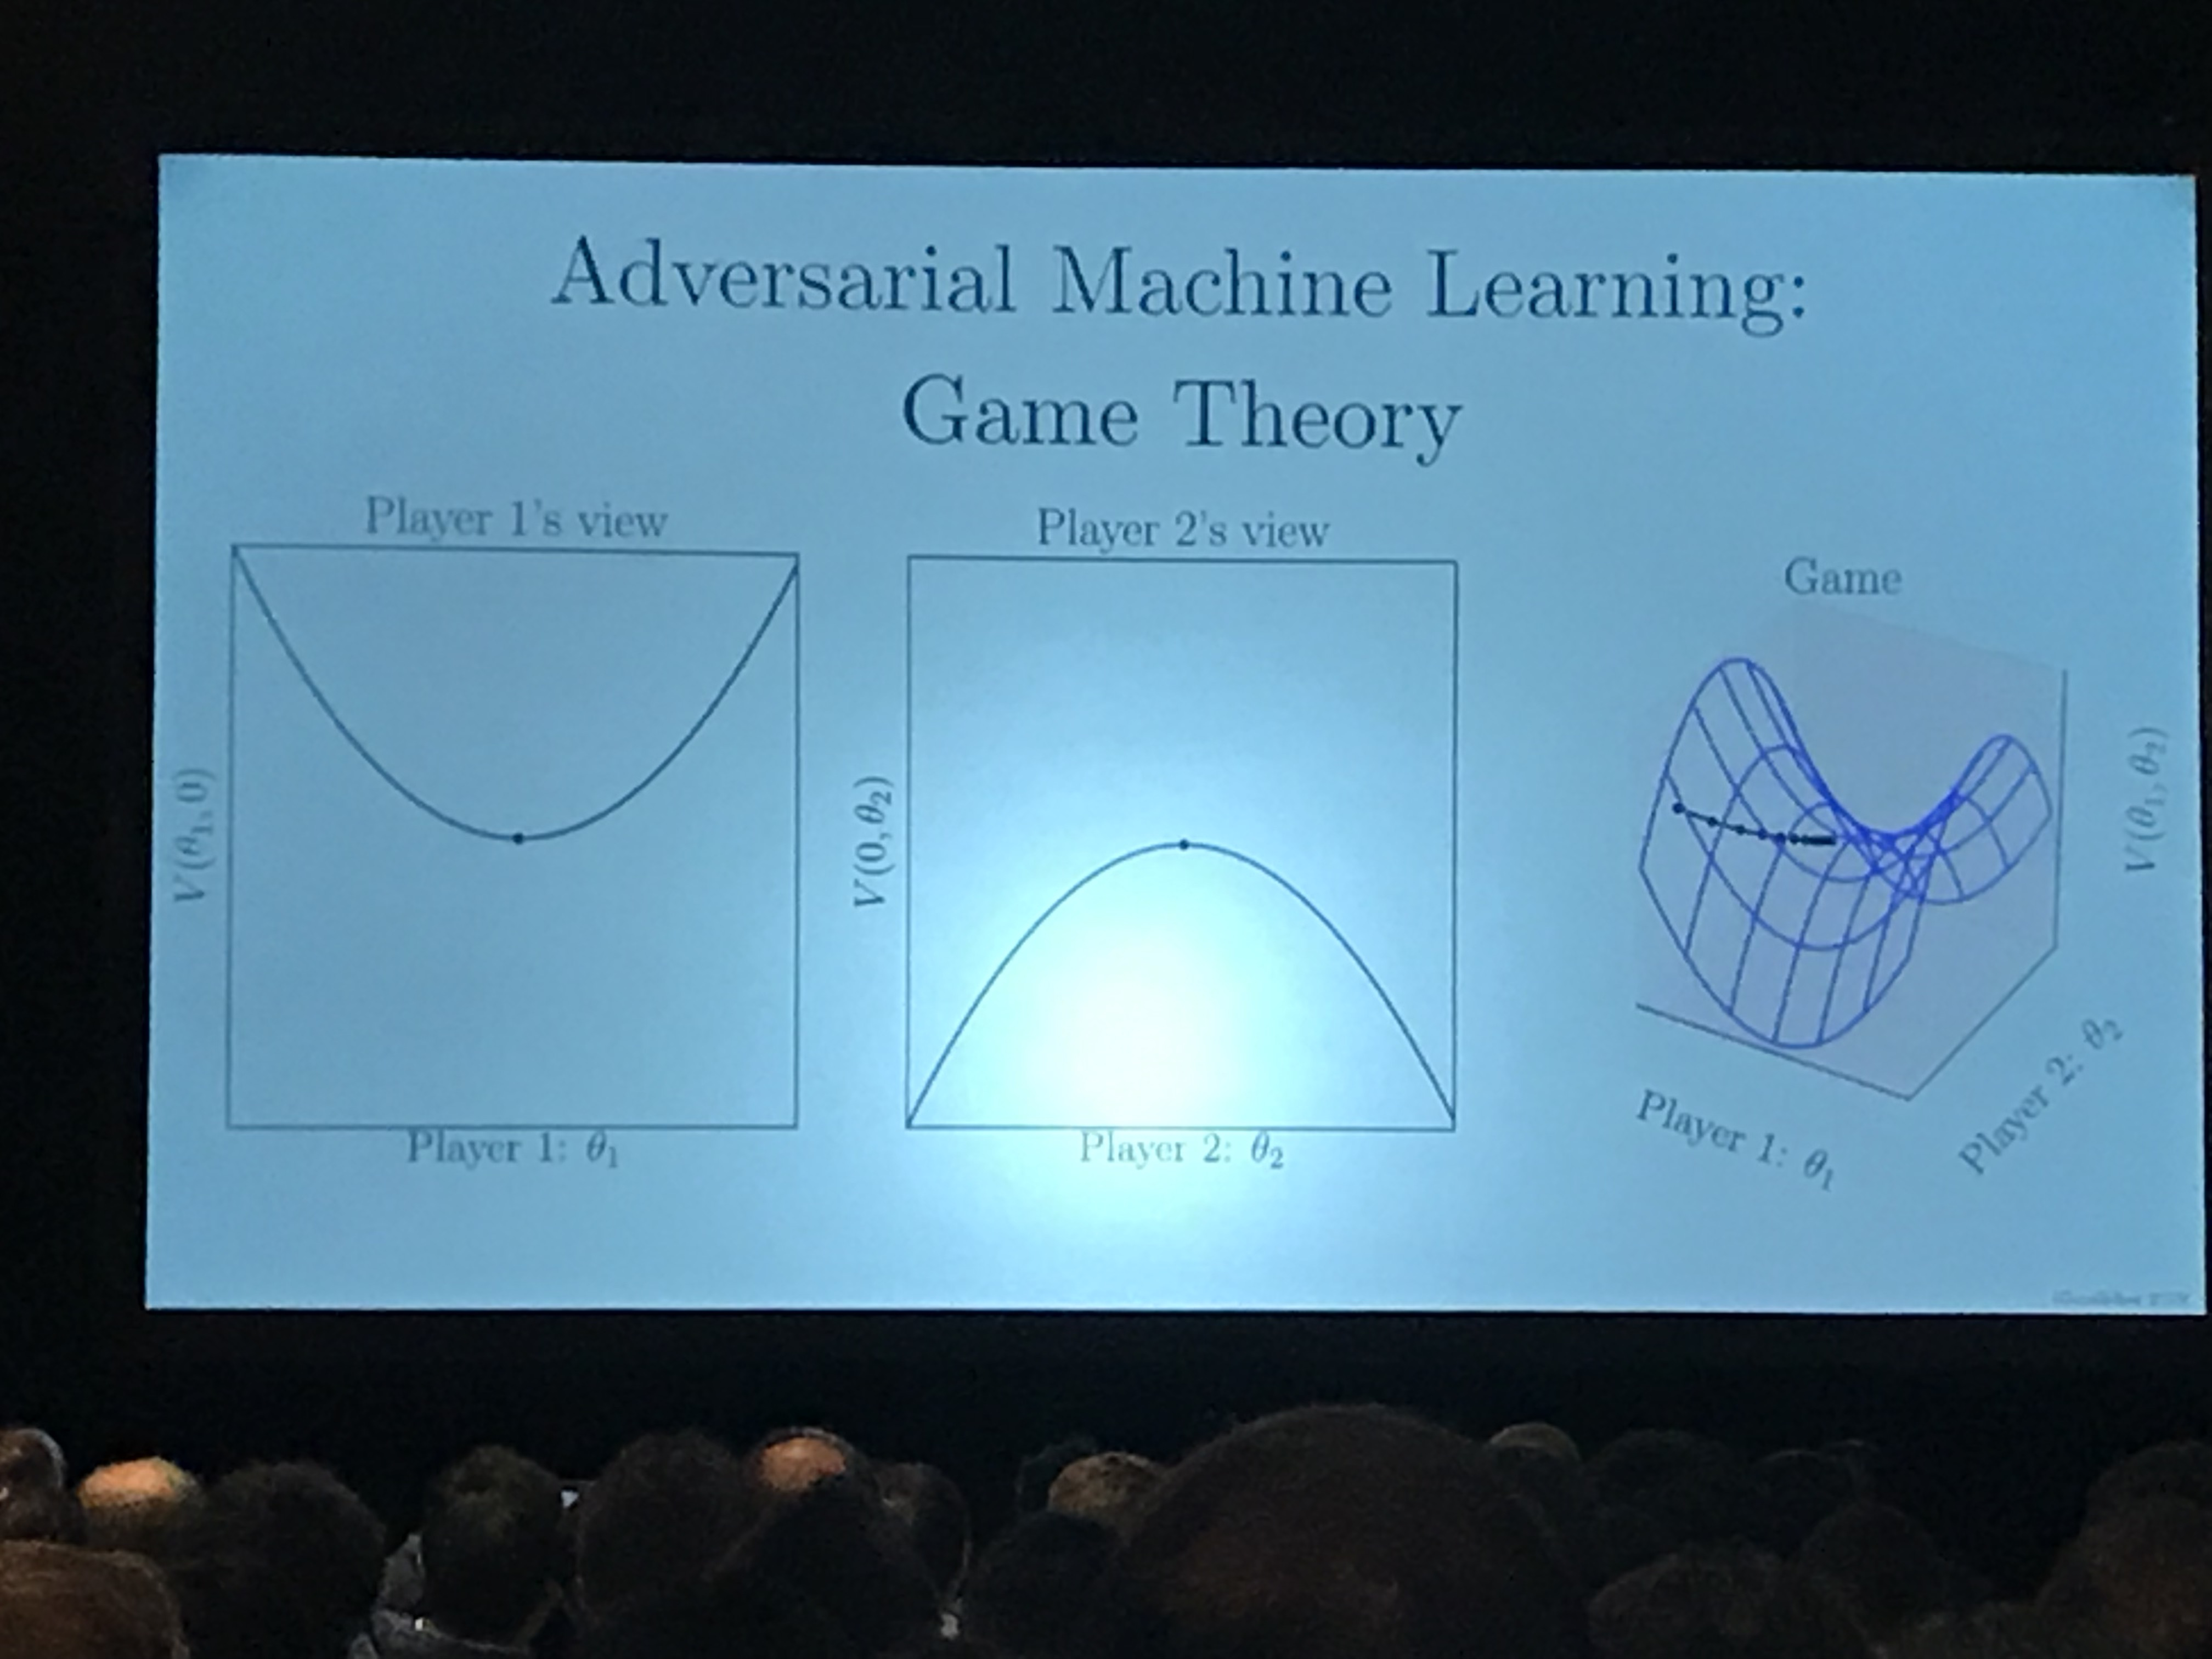
\includegraphics[width=0.5\textwidth]{images/game.JPG}
    \caption{Game theory and optimization.}
    \label{fig:games}
\end{figure}

Cambrian explosion of ML research topics: used to be (2007), let's get ML to work! Then we can do vision/NLP and so on. Now, with ML working, we can go on to do loads of other things (neuroscience, security, RL, domain adaption, and so on). \\


\subsubsection{Generative Modeling}

Main idea: take a collection of training data, and learn a distribution that can generate similar samples~\cite{karras2017progressive}. \\

Use Generative Adversarial Nets (GANs)~\cite{goodfellow2014generative}. Train a 1) generator to generate images, starting out random and a 2) discriminator, to recognize fake images from real images. These two play a game to convergence.

\begin{figure}[h!]
    \centering
    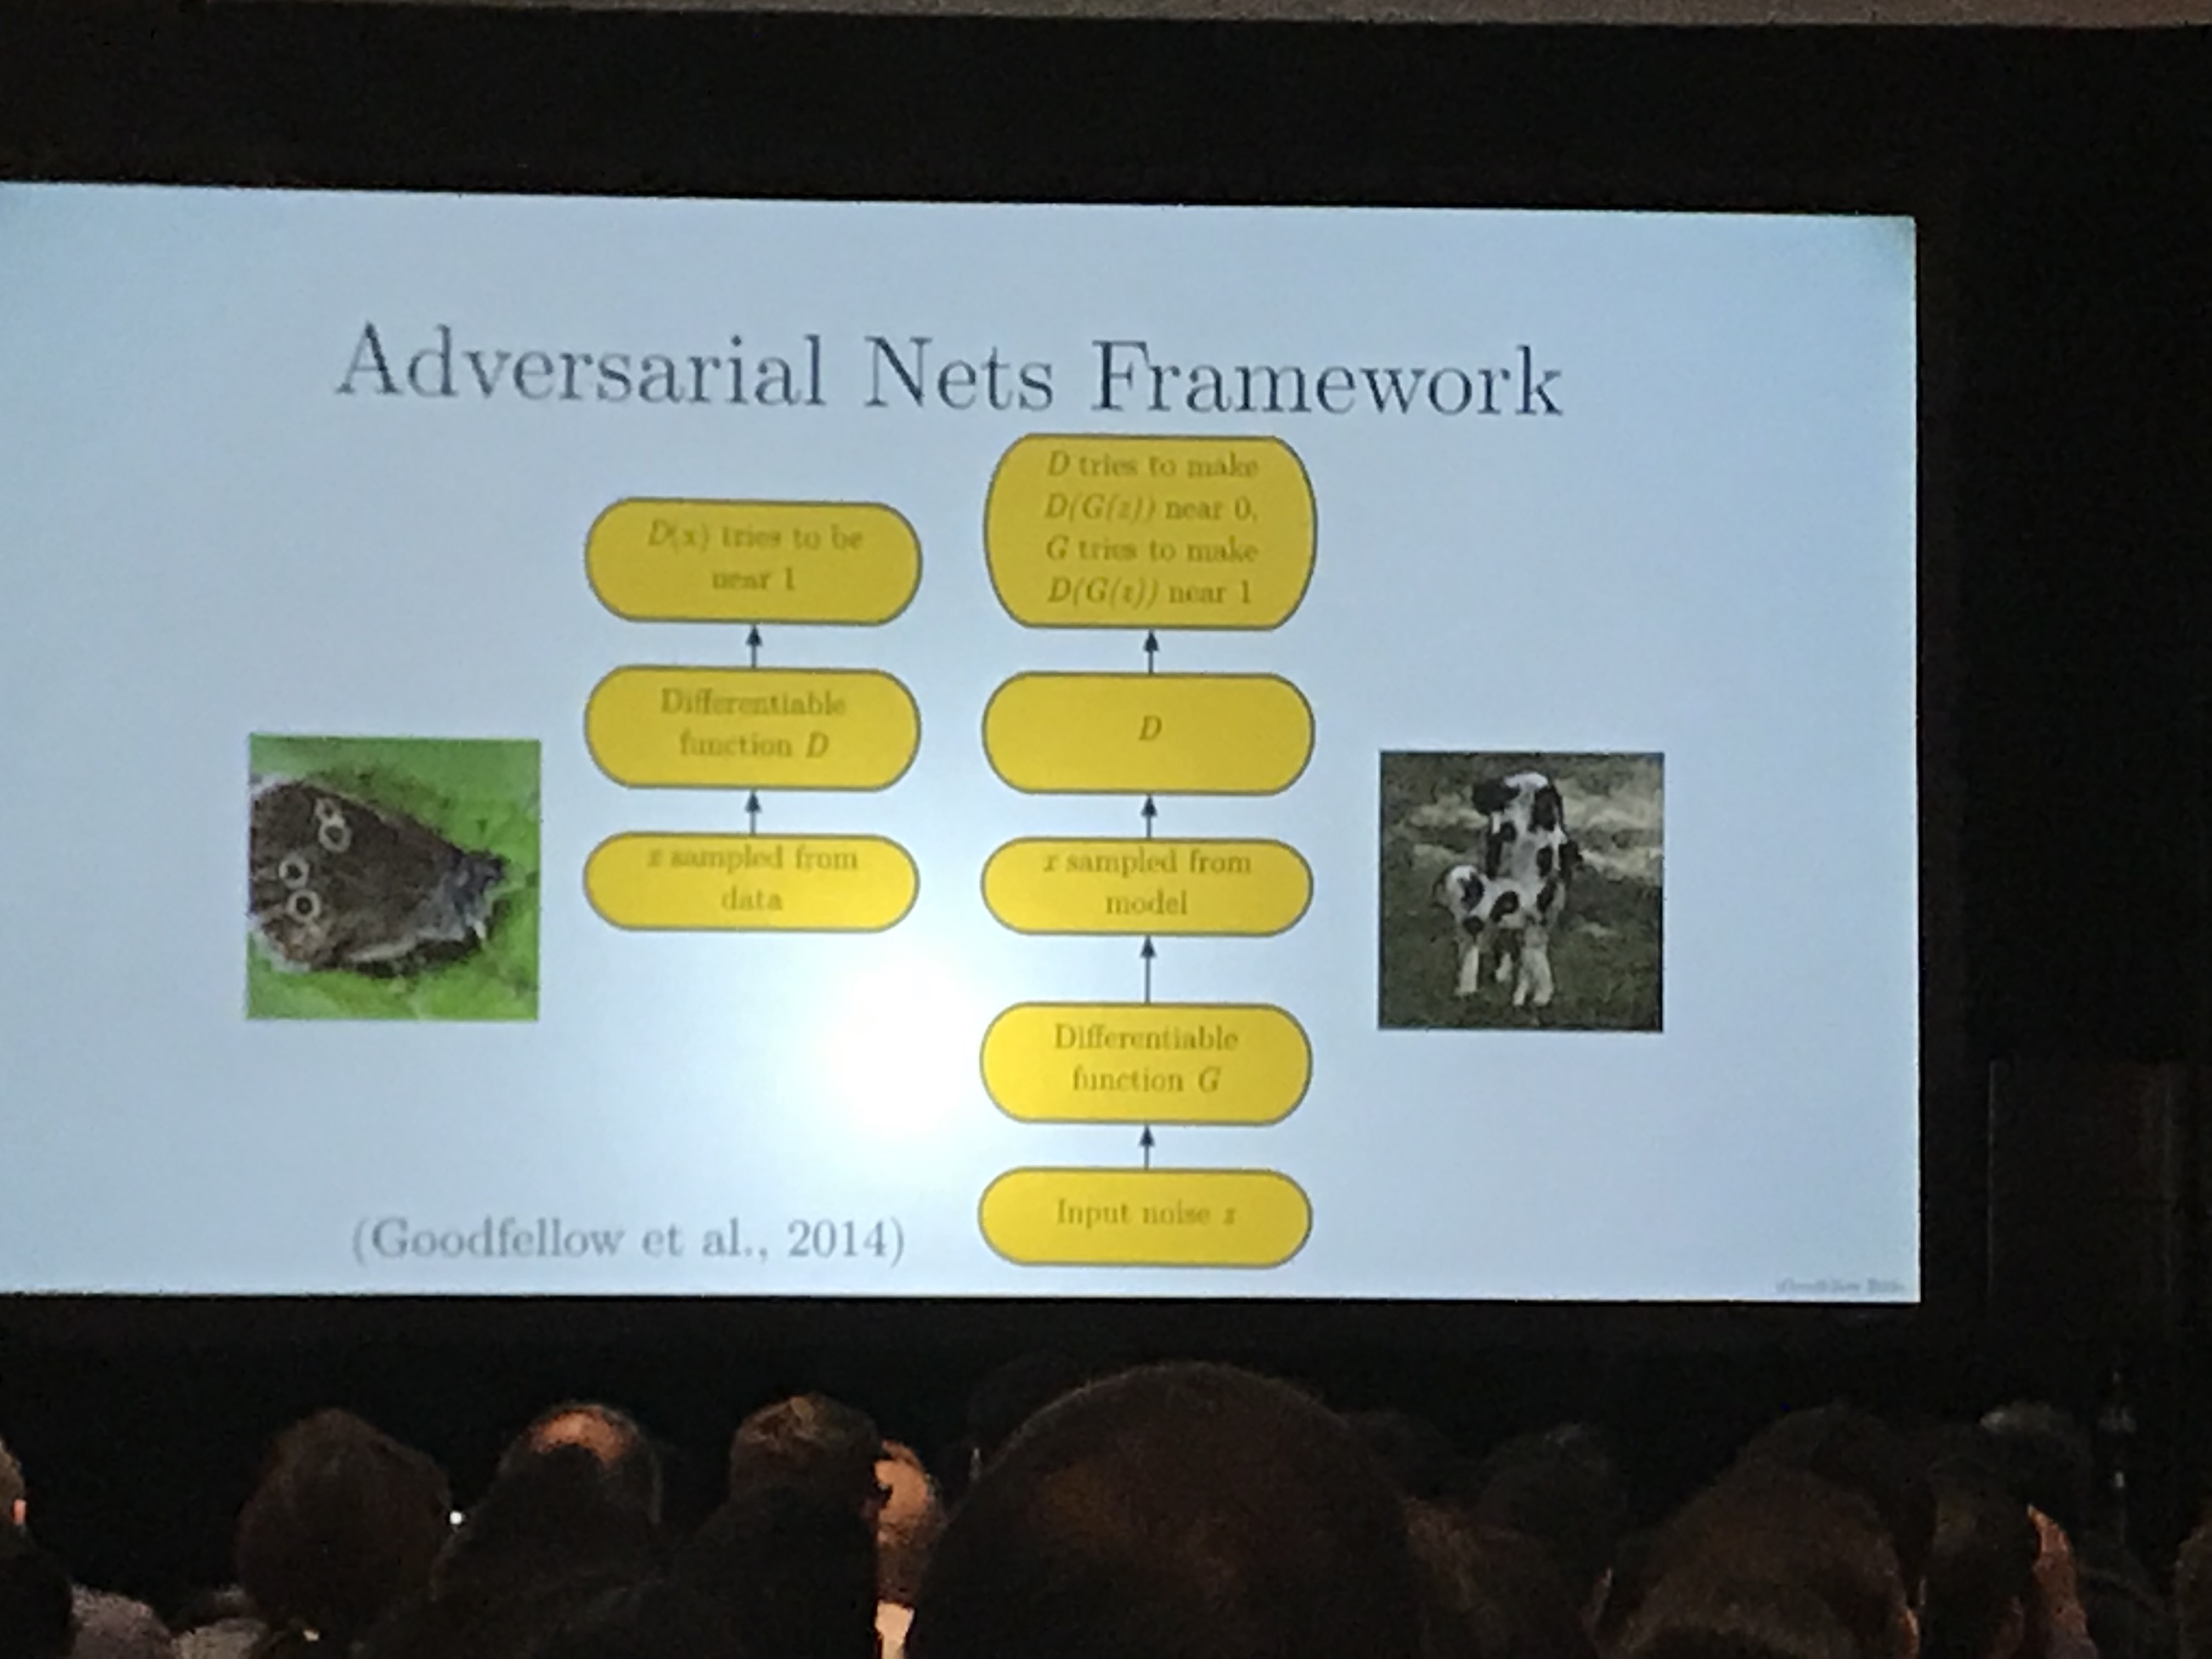
\includegraphics[width=0.5\textwidth]{images/gans.JPG}
    \caption{GAN Framework.}
    \label{fig:gan}
\end{figure}

Rapid progress in image generation (and especially faces -- see Figure~\ref{fig:gan_prog}). Also progress in imagenet, but it's harder because so many more classes. \\


\begin{figure}[h!]
    \centering
    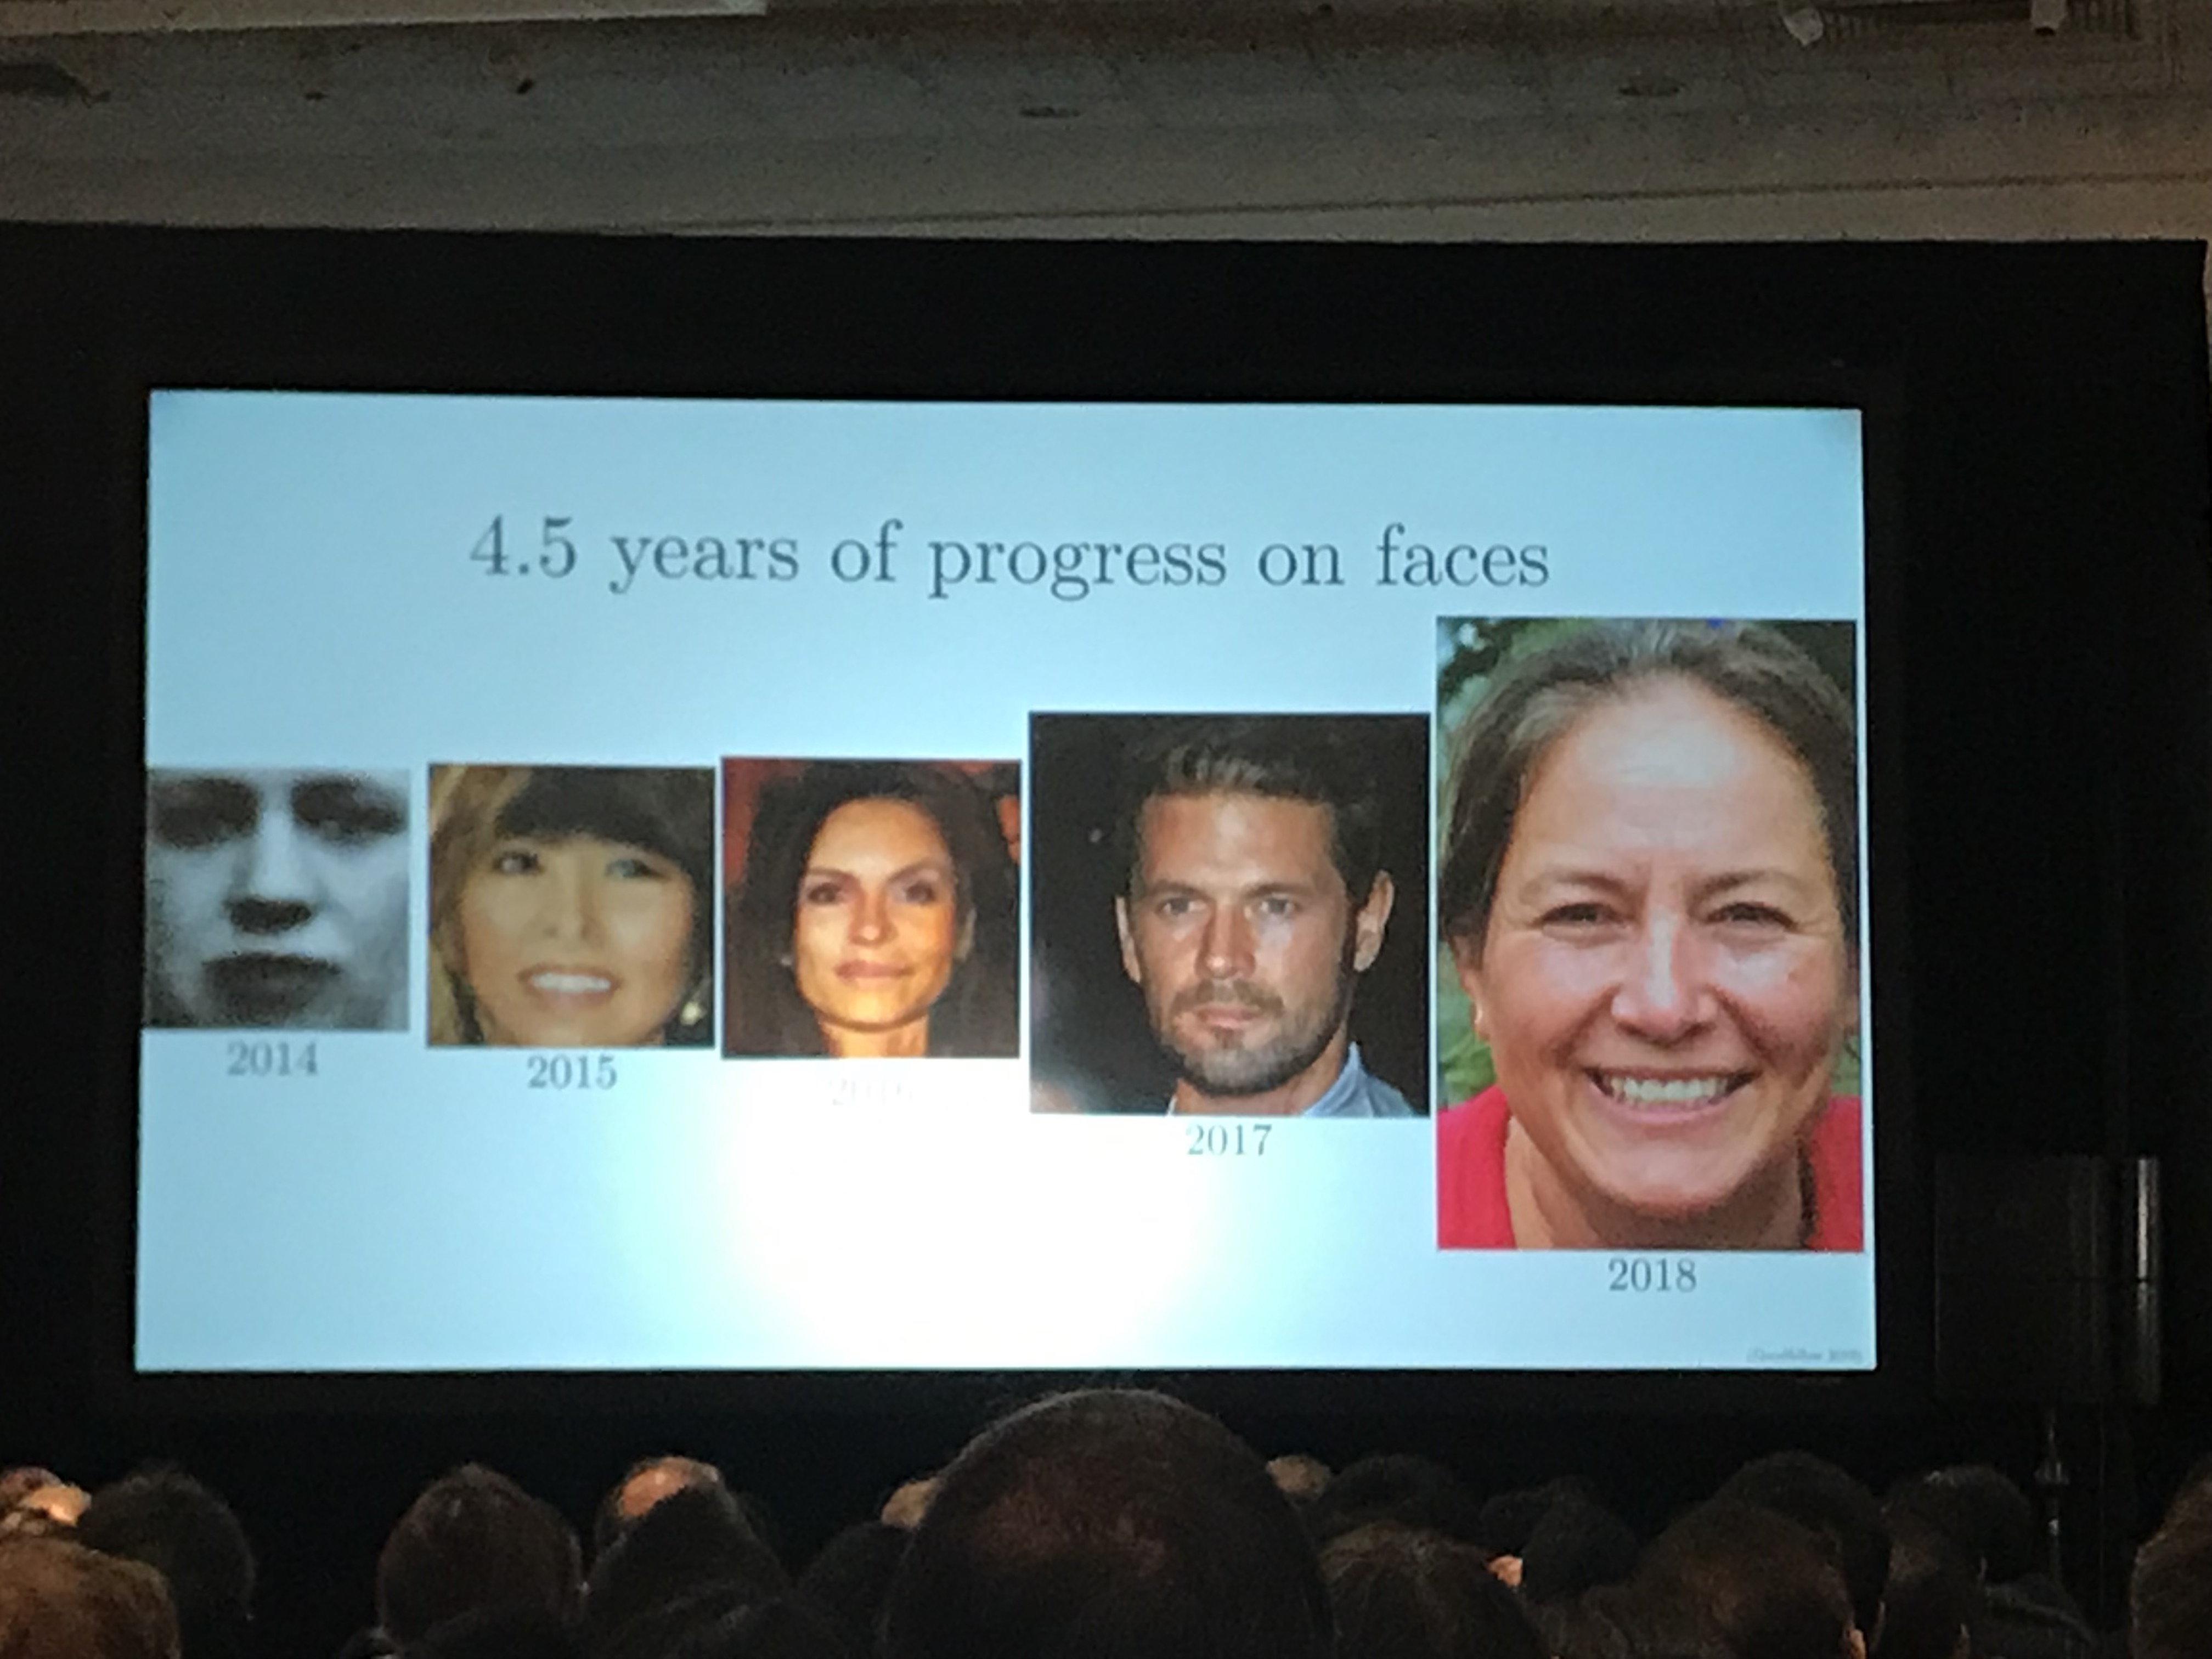
\includegraphics[width=0.5\textwidth]{images/gan_progress.JPG}
    \caption{GAN Progress.}
    \label{fig:gan_prog}
\end{figure}


GANs solve the generative modeling problem, but also the domain translation problem -- can translate video stream during the day to video streams at night {\it without paired day-night examples}. \\

Cool example: cycleGan~\cite{zhu2017unpaired} converts horses to zebras. Also lets us diagnose some issues with the techniques -- CycleGAN only does image-to-image, so it's not targeting video coherence. Also picks up on 


\begin{figure}[h!]
    \centering
    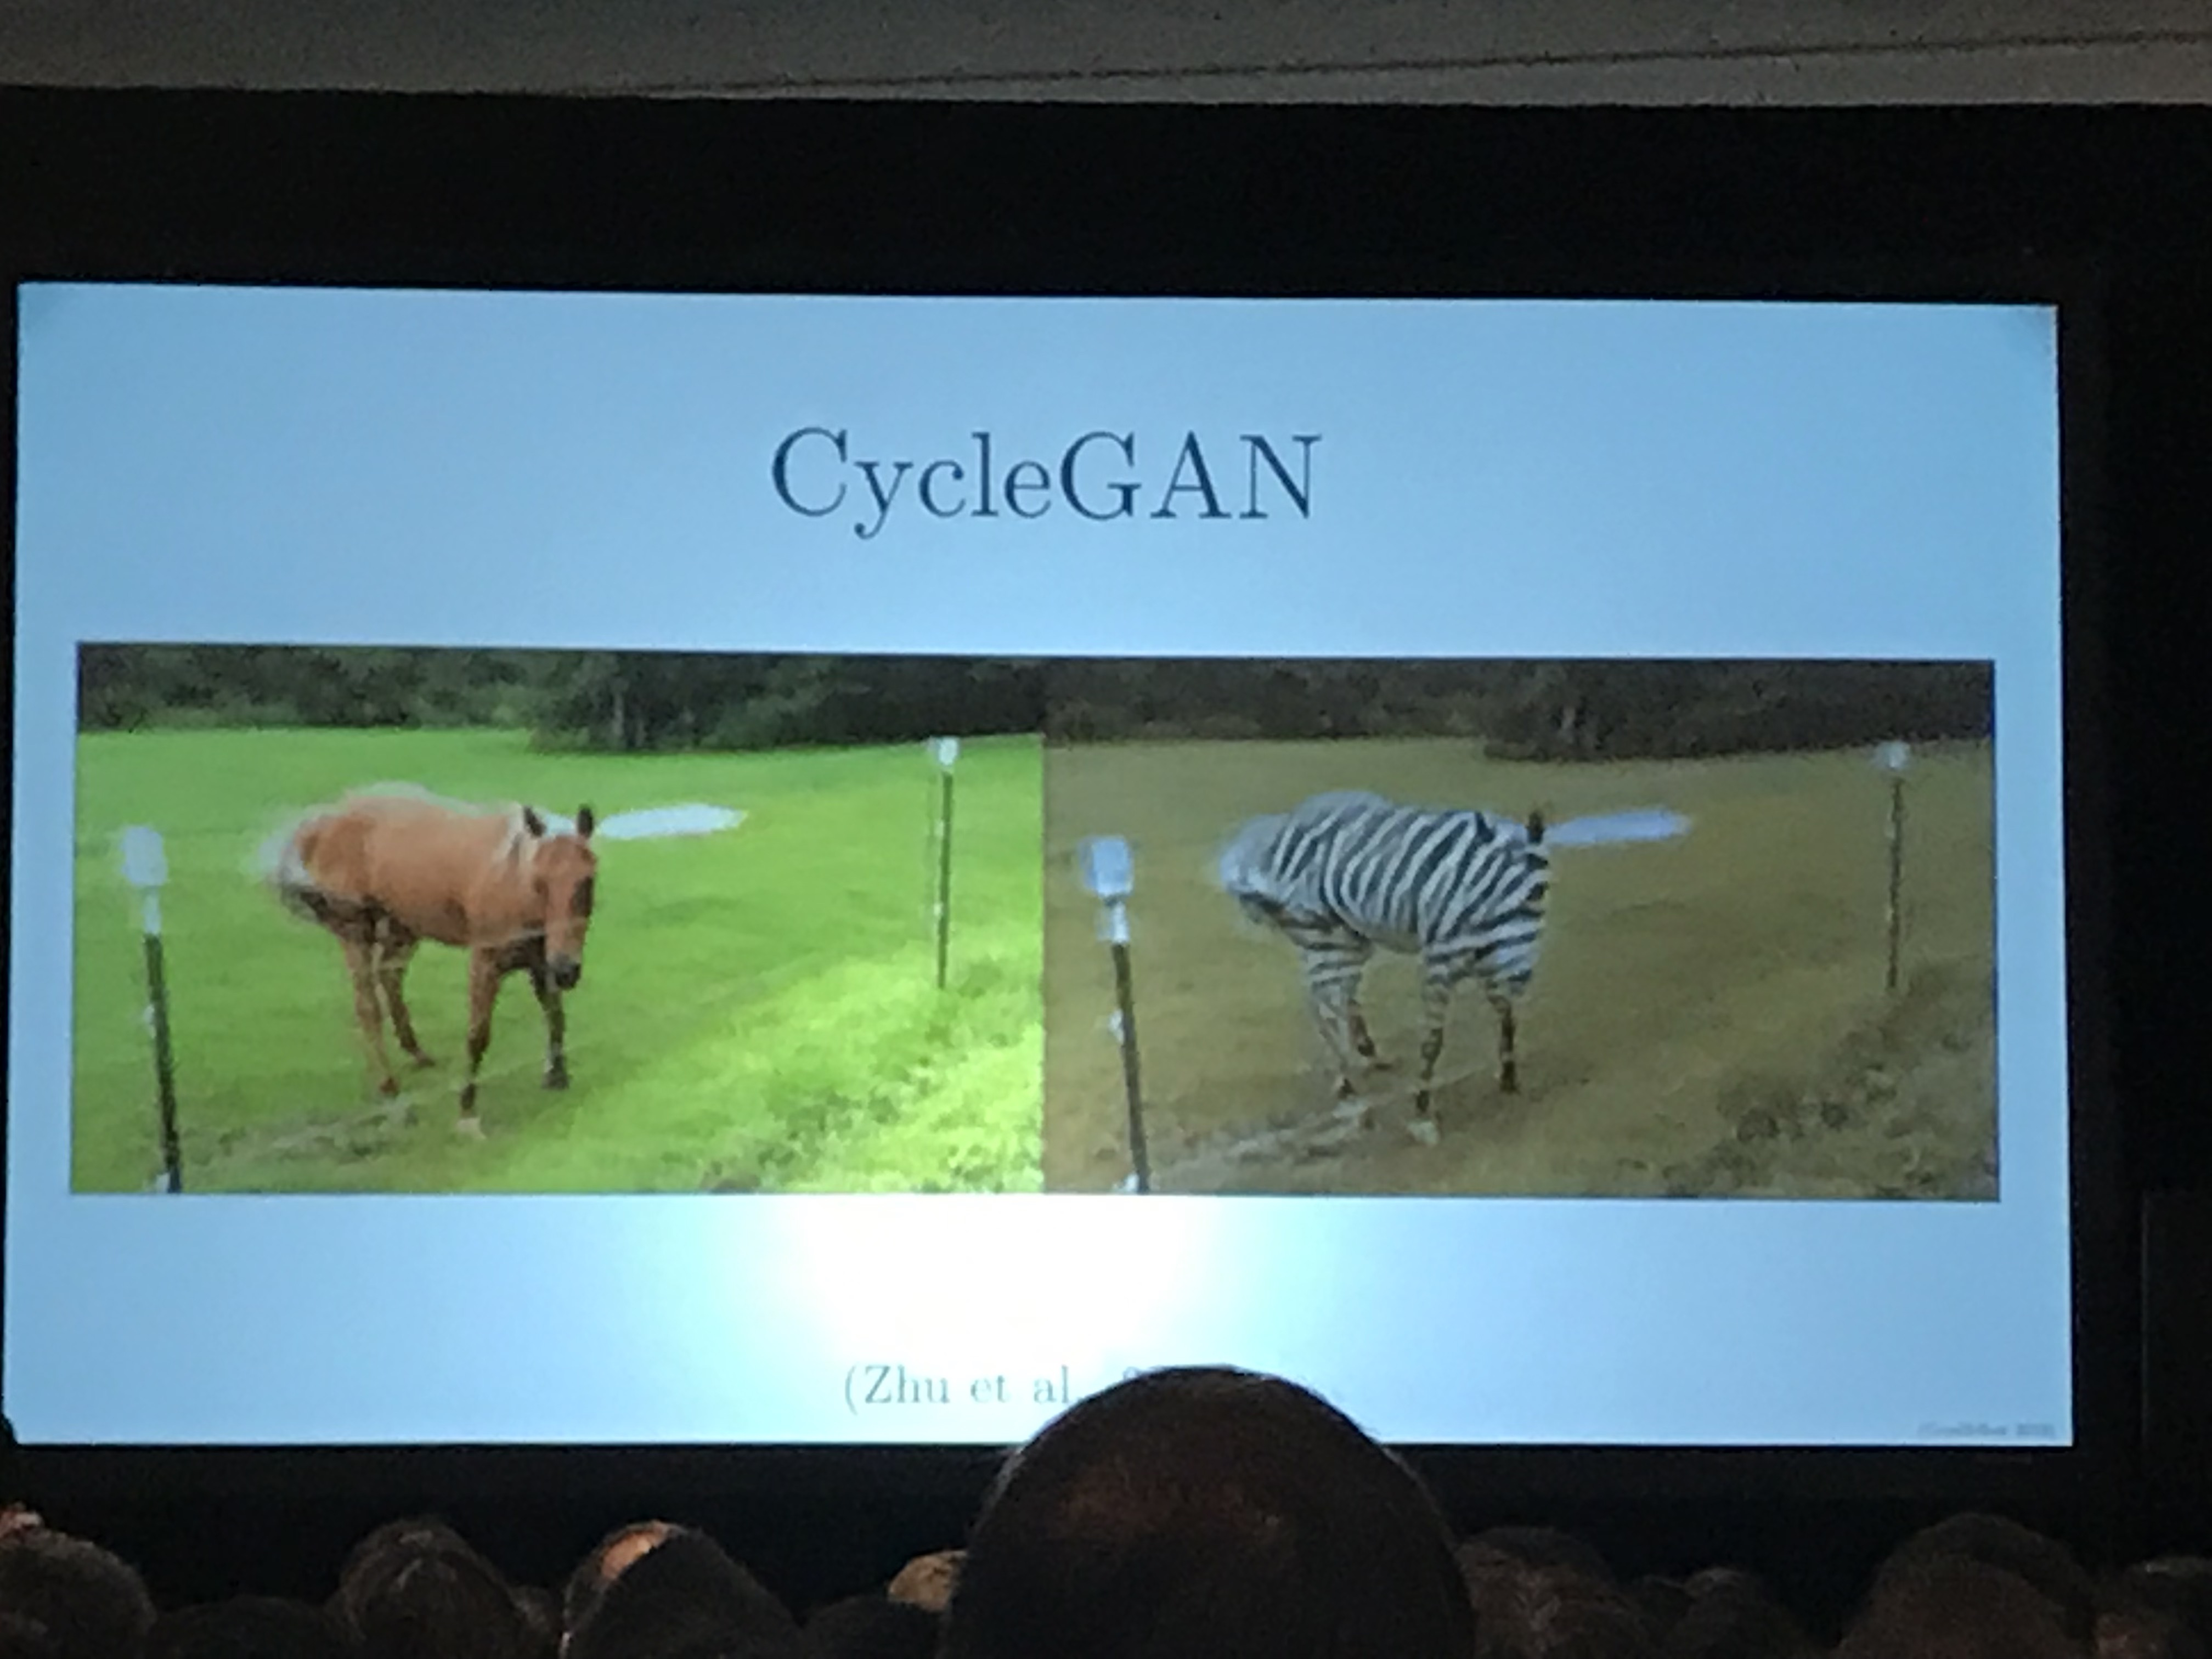
\includegraphics[width=0.5\textwidth]{images/zebra.JPG}
    \caption{CycleGAN turns horses into zebras (actually a video).}
    \label{fig:zebra}
\end{figure}

Also showed an {\it amazing} video of a fake/animated dancer that can be used to change video stream of people to dance in that style. \\

{\bf Application:} New company that generates custom made dental crowns very quickly, which dramatically improves over the traditional method for making crowns. \\

{\bf Prediction:} Fashion! Should be possible to generate clothing that fits well/satisfies individual tastes. \\

\subsubsection{Recent Developments}

Basically: ML works now! So we can do all sorts of cool things, including:
\begin{itemize}
    \item Security
    \item Model-Based Optimization
    \item Reinforcement learning
    \item Fairness and accountability
    \item Neuroscience
\end{itemize}


First, some new ideas in GANs:
\begin{itemize}
    \item Self-Attention~\cite{wang2018non}: Attention mechanism you can add to a CNN that lets you focus on other parts of previous layers' feature maps, given a piece that the network just generated~\cite{} -- so, when it generates an eye of an animal, you can highlight the eye and see what it was focused on.
    
    $\ra$ Not constrained to any shape of attention region -- it can highlight an arbitrary region.

    \item Also: BigGAN~\cite{brock2018large}, large scale TPU implementation. Can generate images at high resolution that are good enough to fool human observers.
\end{itemize}


{\bf Security:} \\

Adversarial Examples! We think these are the result of assuming i.i.d. data -- attackers can violate both ``i" assumptions. \\

$\ra$ attacker can choose examples not drawn from the same distribution (stop sign with graffiti, putting an apple in a mesh bag).
$\ra$ attacker can violate independence, too, to fool a model. \\

These completely work in the physical world too. \\

Advervarsarial training as a minimax problem:
\[
\theta^* = \argmin_\theta \bE_{x,y} \max_\eta[J(x,y,\theta) + J(x+y,\eta, \theta)]
\]

Open research direction: change the i.i.d. assumption and train on adversarial examples, too. Can often make classifiers more robust to these examples. \\

{\bf Model-Based Optimization:}

Idea: train an ML model, and instead of training it to label new data, we use it to train the search for new data points. \\

$\ra$ DNA Sequence design. \\

{\bf Reinforcement Learning:} \\

Recent work identifies adversarial examples for RL, too! \\

But, we can also use GANs to help RL. Consider Arthur Samuel's 1959 checkers player -- used self play to improve itself~\cite{brock2018large}, which is very much in use now. \\

GANs can be used to provide learned reward functions, as in SPIRAL~\cite{ganin2018synthesizing}. Can generate reward functions in the appropriate input domain (robot camera percepts). Usual MSE won't work, but GANs can actually provide a useful distance measure such that a robot can learn to solve robot problems. \\

{\bf Extreme Reliability:} We want extreme reliability for medical diagnosis, surgery robots, and other safety critical domains. \\

$\ra$ Adversarial machine learning might be able to produce extremely reliable systems because they are explicitly trained to be robust to attacks. \\

Virtual Adversarial Training~\cite{miyato2018virtual}: take an unlabeled example, but we know that it ought to be labeled the same whether or not an adversary messes around with it. Works {\it extremely} well for semi-supervised learning (sample efficient, regularizes well). \\

{\bf Domain Adaptation:} We train in one domain (perhaps where data is abundant) and test in another domiain. \\

$\ra$ A ``domain" here is a particular choice of distribtion for training -- ImageNet, videos of people walking down a street, and so on. \\

$\ra$ If we can achieve domain adaptation, pretty good evidence for reliable/robust generalization. \\

One main approach: Domain adaptation networks~\cite{ganin2016domain}. Idea: try to recognize the domain itself, which forces the discriminator to generalize well. \\

Another important instance of domain adaptation focuses on transferring from {\it simulated} training data to {\it real} data. Works well with recognizing where eyes are looking, for instance. \\

$\ra$ Can do robot grasping by training simulation and then actually grasp in the real world.\\

{\bf Fairness, Accountability, Transparency:} GANs can learn more fair representations \\

$\ra$ Fairness: An adversary tries to infer a sensitive variable $S$ from a representation. Learner tries to learn while making $S$ impossible to recover~\cite{edwards2015censoring}. \\

$\ra$ Transparency: Interpretability and adversarial learning should talk more. Interpretability means getting the right answer, while adversarial training means the learner is getting the ``right" thing. \\

{\bf Neuroscience:} \\

Adversarial examples affect both computer and time-limited human vision:

\begin{figure}
    \centering
    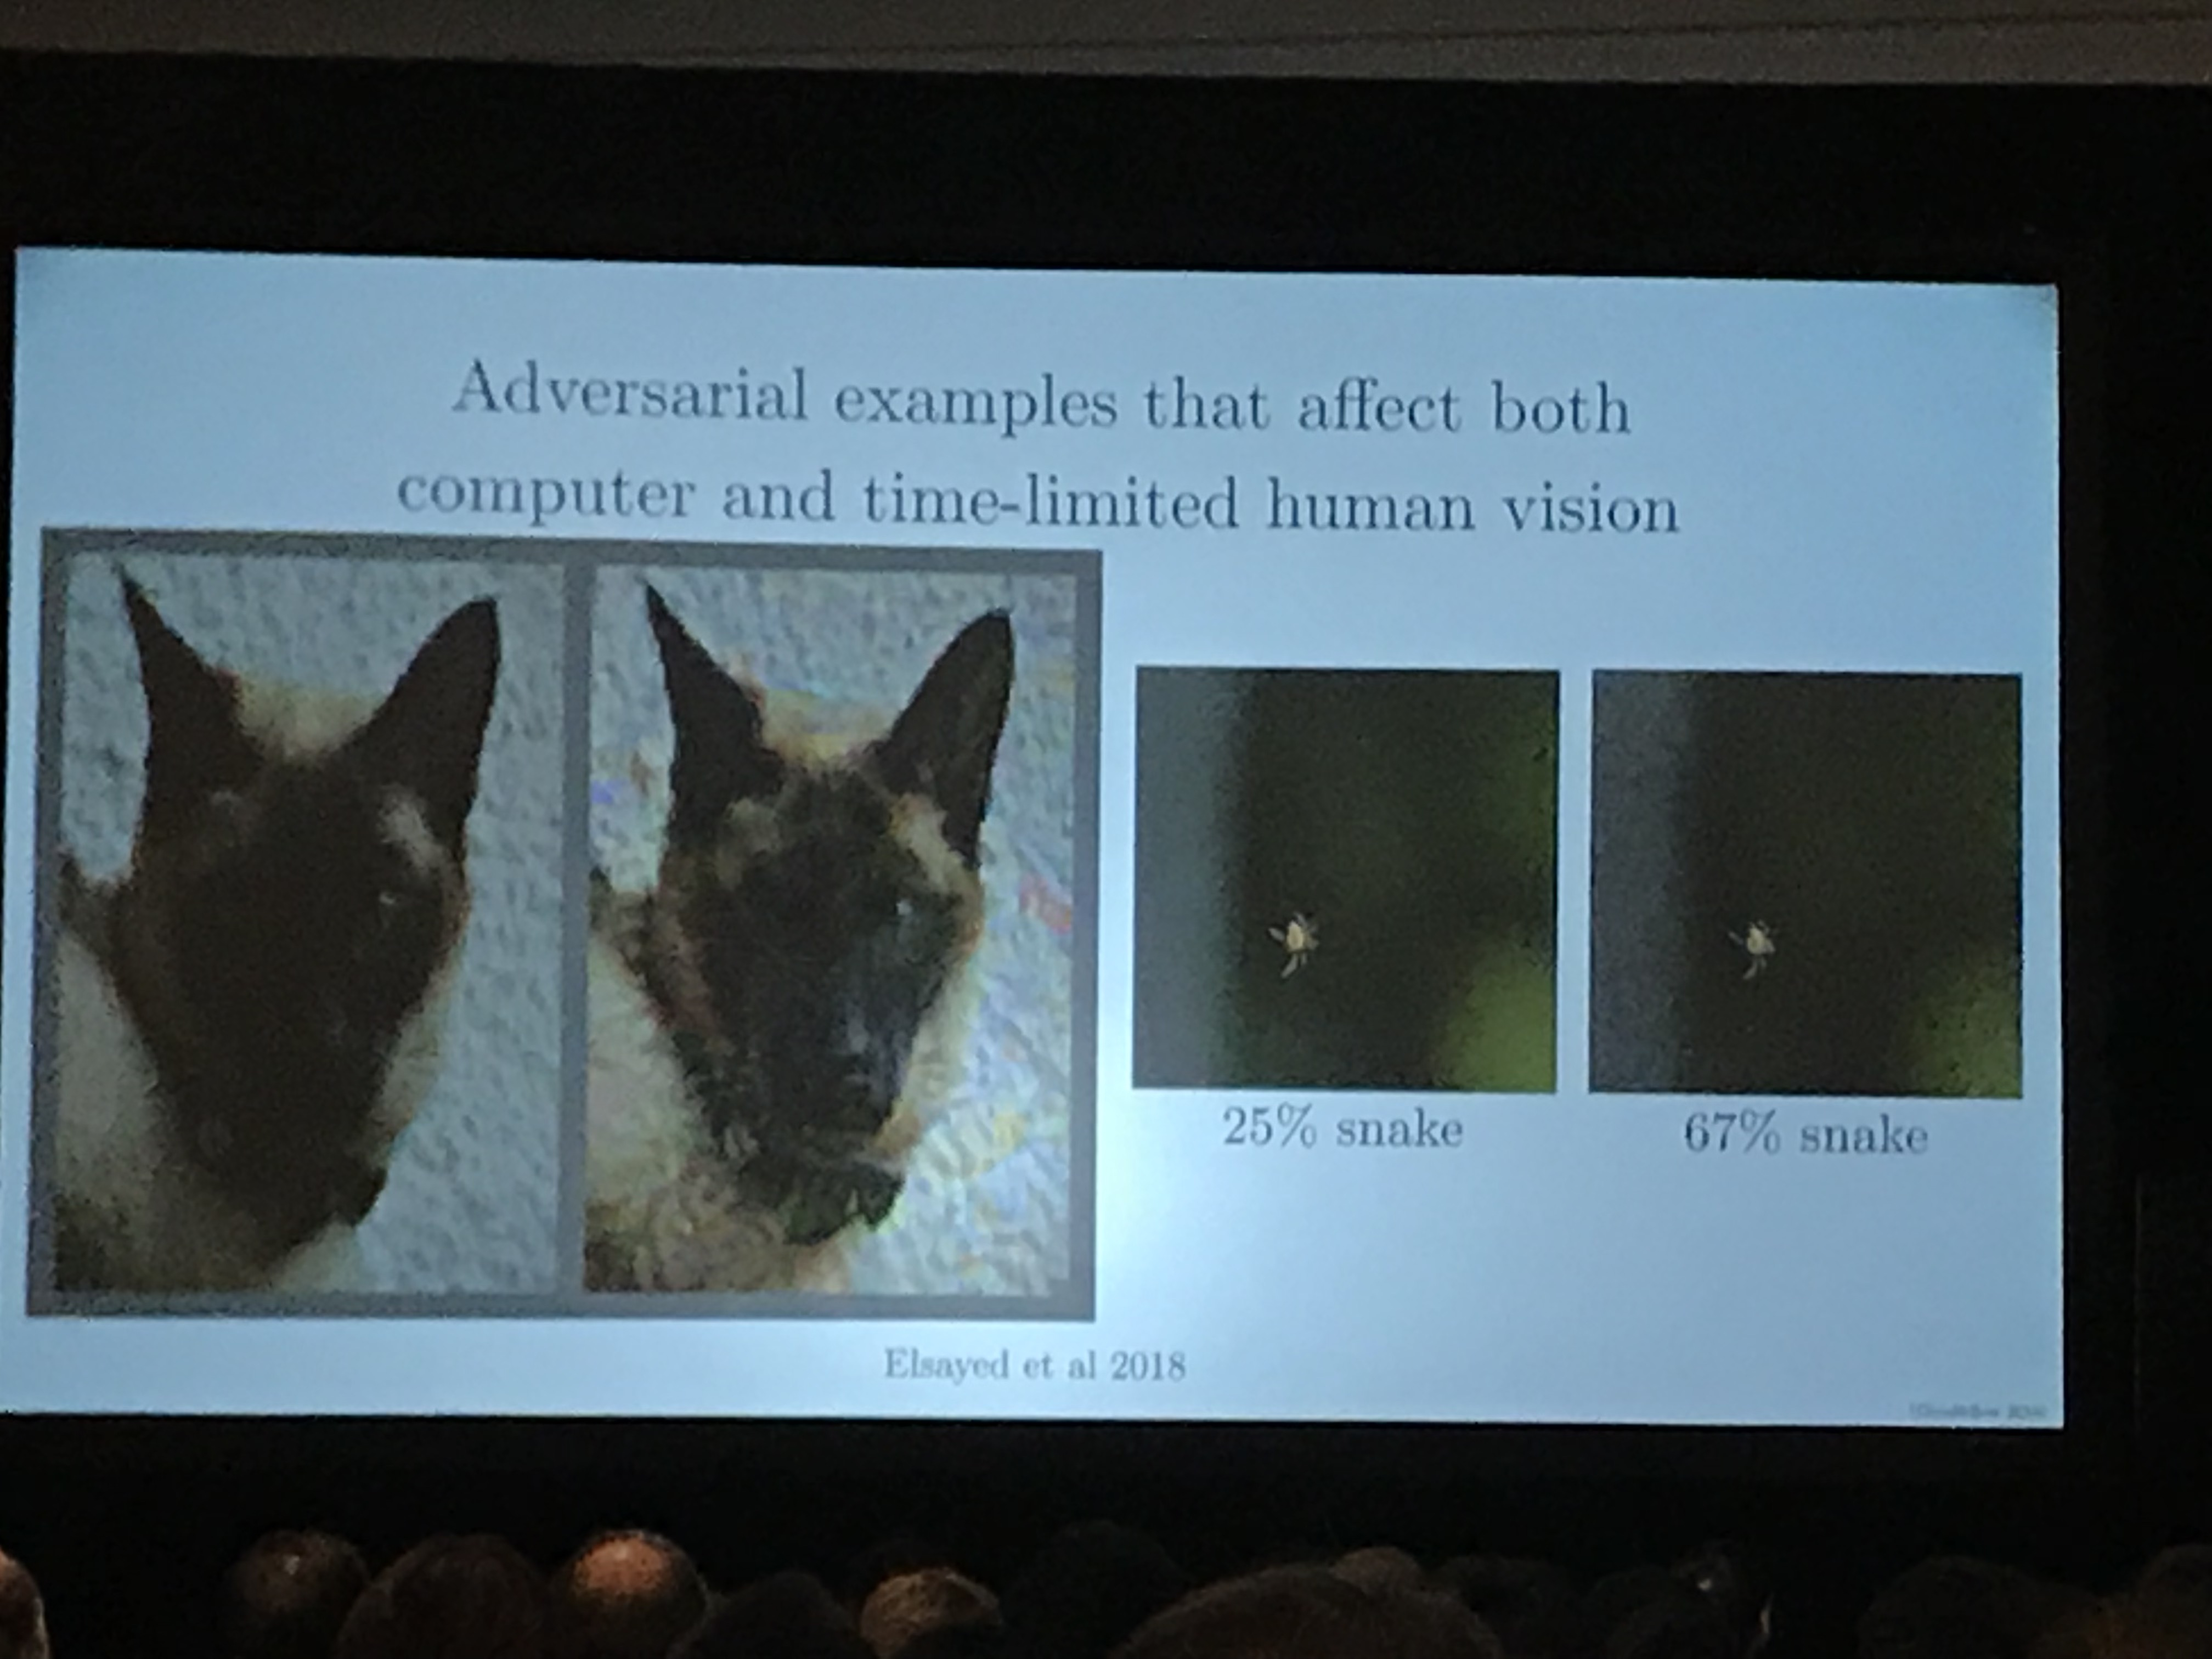
\includegraphics[width=0.5\textwidth]{images/dog.JPG}
    \caption{People are also prone to adversarial examples, too}
    \label{fig:dog}
\end{figure}

\spacerule

\dnote{I have meetings now until the RL session.}

\subsection{Reinforcement Learning}

Now for some RL! (yay!) \\

\subsubsection{Virtual Taobao: Online Environment for RL~\cite{shi2018virtual}}

Paper by Jing-Cheng Shi1, Yang Yu1, Qing Da, Shi-Yong Chen, An-Xiang Zeng. \\

RL is sample inefficient -- so, good virtual environments can be useful. \\

Recommendation in TaoBao is an RL problem. Taobao is an online store like Amazon -- actions involve clicking around, searching, looking at products/reviews, and so on. \\

Claim: RL in TaoBao is infeasible. \\

{\bf Problem:}
\begin{itemize}
    \item User sends search request (can also click/pay/leave).
    
    $\ra$ Goal: optimize customer preference
    
    \item TaoBao displays request (via a ranking policy, $\pi$).
    
    $\ra$ Goal: Maximize performance
\end{itemize}

Main contribution:
\begin{itemize}
    \item Use a GAN-SD (?) to learn a simulated customer policy. Does a good job of simulating the customer's distribution (\dnote{over states? actions? I wasn't sure}).
    \item Then do Multi-Agent Imitation Learning (MAIL) to learn customer shopping policy under a dynamic platform.
    \item Evaluated on TaoBao.
\end{itemize}

\subsubsection{QUOTA: Quantile Option Architecture~\cite{zhang2018quota}}

Distributional RL: Learns a {\it distribution} over the return instead of just the mean. \\

Standard RL: learns $v(s;\theta) \ra \bE[R(\theta)]$. \\

Distributional RL: learns full distribution, $\mc{N}(\mu,\sigma^2)$. \\

{\bf Research Question:} Why need distributional RL?\\

$\ra$ Main answer: can derive risk sensitive policies to explore more effectively. \\

Quantile encoding of a distribution encode {\it rank statistics} of a distribution. Use the median of each quantile to represent that segment. \\

{\bf Quantile-DQN:} Maps each $(s,a)$ to a value distribution of that state-action pair (extension to DQN). \\

Action selection is usually {\it based on the mean} of this distribution. Test on Atari, works better than DQN. Also test on ``roboschool" (similar to mujoco). Also works. \\



Instead: select based on the $k$-th quantile:
\[
a_t = \argmax_a q_k(s,a),
\]
where $k$ is the $k$-th quantile of the value distribution. \\

Bencmarked several algorithms in a simple chain domain to gain intuition -- compare a ``pessimistic"-QR vs. ``optimistic-QR". Can encode optimism/pessimism via choosing high/low quantile. \\

QUOTA: Hierarchical formulation where each quantile is an option.

\subsubsection{Combined RL via Abstract Representations~\cite{franccois2018combined}}

Paper by Vincent Fran{\c{c}}ois-Lavet, Yoshua Bengio, Doina Precup, and Joelle Pineau.\\

{\bf Goal:} Combine model-based and model-free RL to do hierarchical RL. \\

\ddef{Model-basedRL}{learn a model and do planning to compute $Q$.}

\ddef{Model-free RL}{learn $Q$/$\pi$ directly}

Combined! Might be better (more interpretable, sample efficient, and so on). \\

Idea: Combined Reinforcement via Abstract Representations (CRAR). Model-based learns transition function to act, model-free learns value both in an off policy way. \\

Learning: 
$\ra V$, use DDQN.  \\
$\ra T,R$, use an encoder. But! Trivial transition function often learned where all states are abstracted into the same state (which makes $T$ prediction very easy). \\

So, add a regularizer/cost term that encourages more states. \\

Test in a labyrinth task. Yields a meaningful representation that can be visualized in 2dimensions that is interpretable. \\

%Plan based on best estimated $\hat{Q}^*$. \\

Main evaluation on a randomly generated set of labyrinths -- train on a small set of sampled MDPs, then test on a new set of samples. Also do zero-shot transfer on labyrinths. \\

Conclusion:
\begin{itemize}
    \item CRAR can generalize while being efficient
    \item Can work from off policy data
    \item Approach recovers a low-dimensional representation of the environment even in the absence of model-free objective, which is important for 1) transfer, 2) exploration, 3) interpretability.
\end{itemize}

\dnote{Now the poster spotlights, 2 minute highlights}

\subsubsection{Poster Spotlights}

2 minute spotlights:
\begin{itemize}
    \item {\bf Diverse Exploration via Conjugate Policies:} noted that on policy methods suffer from a lack of exploration. Exploration is hard!
    
    $\ra$ solution: diverse exploration. Deploy a set of diverse of exploration policies, where diversity means each policy will behave dissimilarly in each state. 
    
    $\ra$ Contributions: variance analysis of policy gradient objective under these dissimilar exploration policies.
    
    \item {\bf State-Augmentation Transformations:} Look at MDPs in a risk sensitive manner. 
    
    $\ra$ Consider reward functions that take as input $s,a$ {\it and} $s'$. \\
    
    $\ra$ Analzse results if you consider the $(s,a,s')$ based reward function instead of the ``typical" kind. Provide a recipe for translating any transition based MDP to a state based MDP.
    
    \item {\bf Trust Region Evolution Strategies:} Enhance evolution strategies for black box optimization using RL.
    
    $\ra$ Contribution: make more efficient use of sampled data by optimizing surrogate objective function for multiple epochs of updates. Prove guarantees for this next optimization procedure, and a practical algorithm that makes a few approximations.
    
    \item {\bf Comparative Analysis of Expected and Distributional RL:} Where does the advantage of distributuonal RL come from?
    
    $\ra$ Main Q: in what settings does distributional RL behave differently from expected RL?
    
    $\ra$ Conclusions at the poster!
    
    \item {\bf Hybrid RL with Expert State Sequences:} Learning scenario where an RL has access to incomplete but obtainable expert demos.
    
    $\ra$ Propose an efficient dynamics model to infer unobserved actions.
    
    $\ra$ Joint policy optimization via RL and behavioral cloning.
    
    \item {\bf Natural Option Critic:} Builds on Option Critic by combining with Natural Gradients.
    
    $\ra$ Typical Option Critic uses regular gradient which is NOT variant to reparameterization.
    
    $\ra$ Thus, if we extend to natural gradient, we can then do reparameterization, which leads to many practical improvements (without having to invert a matrix).
    
    \item {\bf Utility of Sparse Representations for Control:} Fixed sparse representation like tile coding has been effective for control, but is not scalable b/c number of features explodes.
    
    $\ra$ Goal here is to learn a sparse representation with neural networks (last layer has {\it sparse} activations).
    
    $\ra$ Sparse representation is scalable to high dimensional inputs and is indeed helpful for RL.
    
    
\end{itemize}




% --------------
% -- Thursday --
% --------------
\section{Thursday January 31st}
Next up, the joint IAAI/AAAI talk on smart cities.

\subsection{Invited Talk: Yu Zheng on Smart Urban Cities}

Consider: Rapid Progress of urbanization. Has led to huge challenges in dense urban areas, from traffic to housing. \\

{\bf Vision:} Use urban computing to improve lives in cities through:
\begin{itemize}
    \item Urban Sensing
    \item Data Management
    \item Data Analytics
    \item 
\end{itemize}

\begin{figure}[h!]
    \centering
    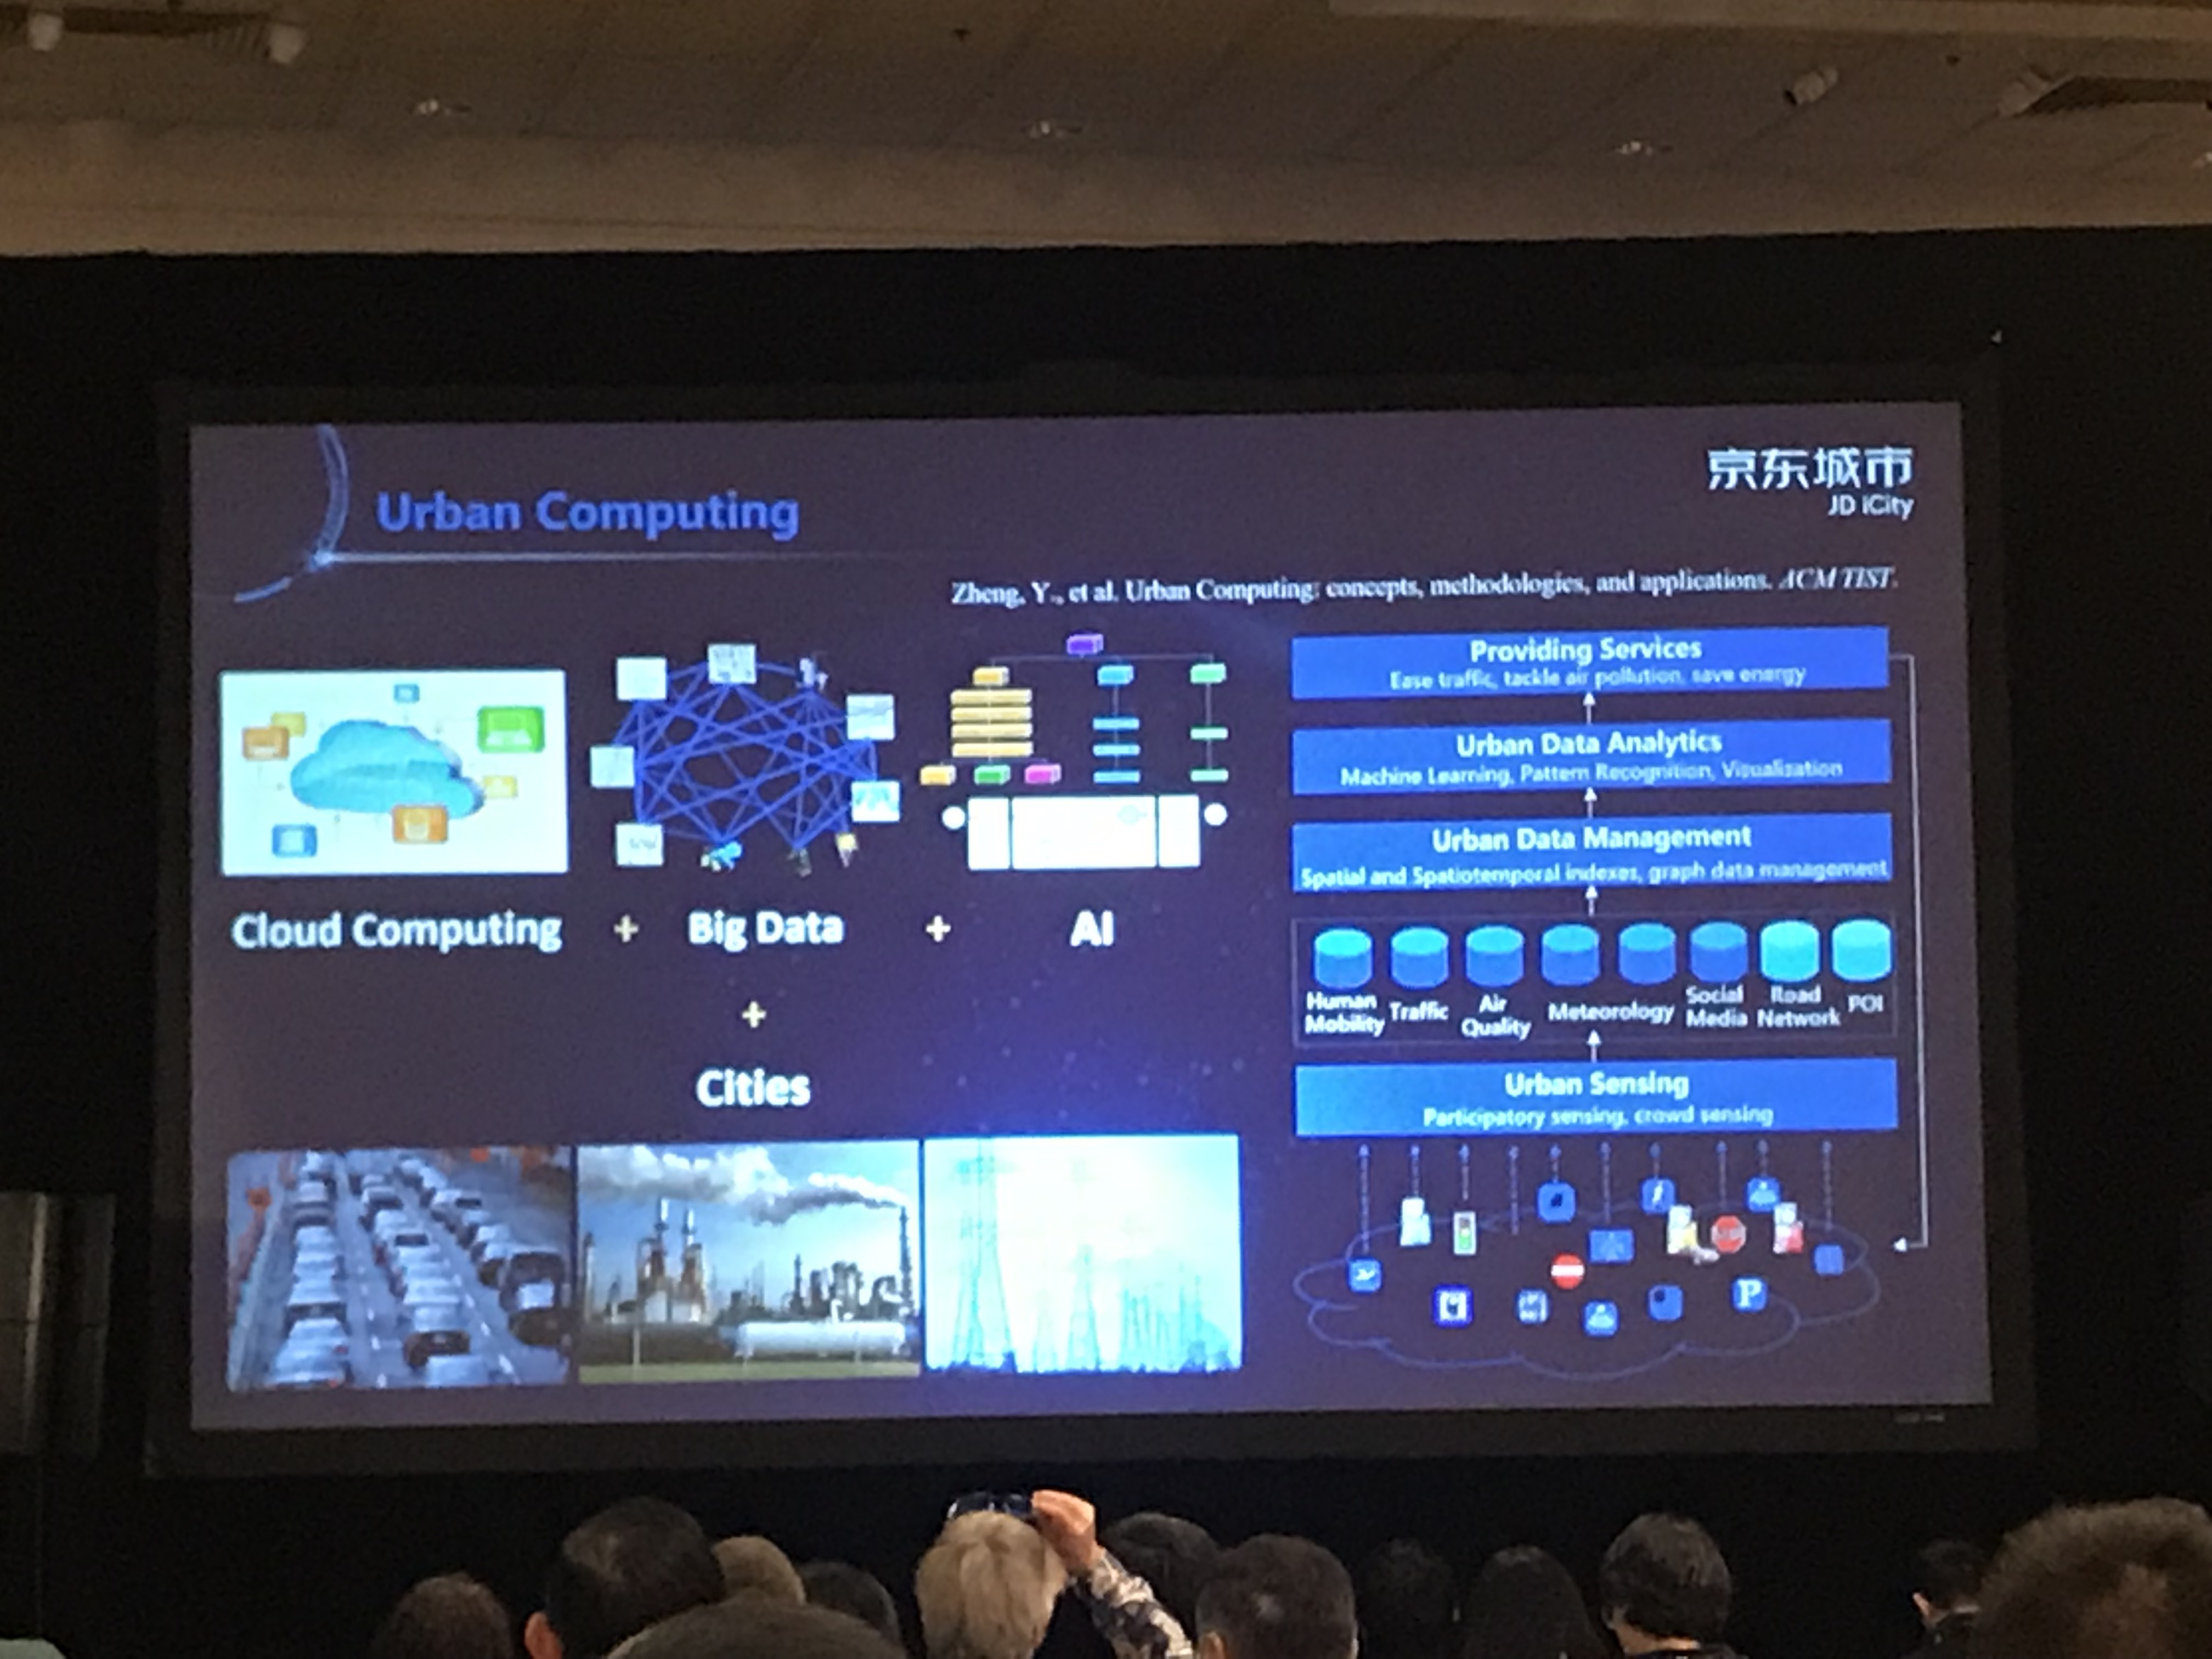
\includegraphics[width=0.5\textwidth]{images/urban.JPG}
    \caption{Overview of urban computing vision.}
    \label{fig:urban}
\end{figure}



\subsubsection{Challenge 1: Urban Sensing}

Challenges:
\begin{enumerate}
    \item {\it Resource deployment:} How should we deploy sensors to gather the right data? Candidate selection is an NP-Hard problem.
    \item {\it Measuring:} Hard to define a measurement for evaluating the deployment
    \item {\it Biased samples:} taxi flow vs. traffic flow. Taxi traffic is biased toward particular routes (but we can get taxi data).
    \item {\it Data Sparsity:} limited air quality sensors but want fine grained air quality throughout a city.
    \item {\it Data Missing:} Communication/sensor errors.
\end{enumerate}

If we can overcome these challenges, we can then collect a diversity of data: air quality, pedestrian traffic, bus use, etc. \\

$\ra$ Summarize data into a particular 6 kind ontology, based on their spatio-temporal type (static, temporal, dynamic, and point-based vs. network based. Goal is to make this scalable so that any new data types can be captured into the future. Summarized in Figure~\ref{fig:data_type}.

\begin{figure}[h!]
    \centering
    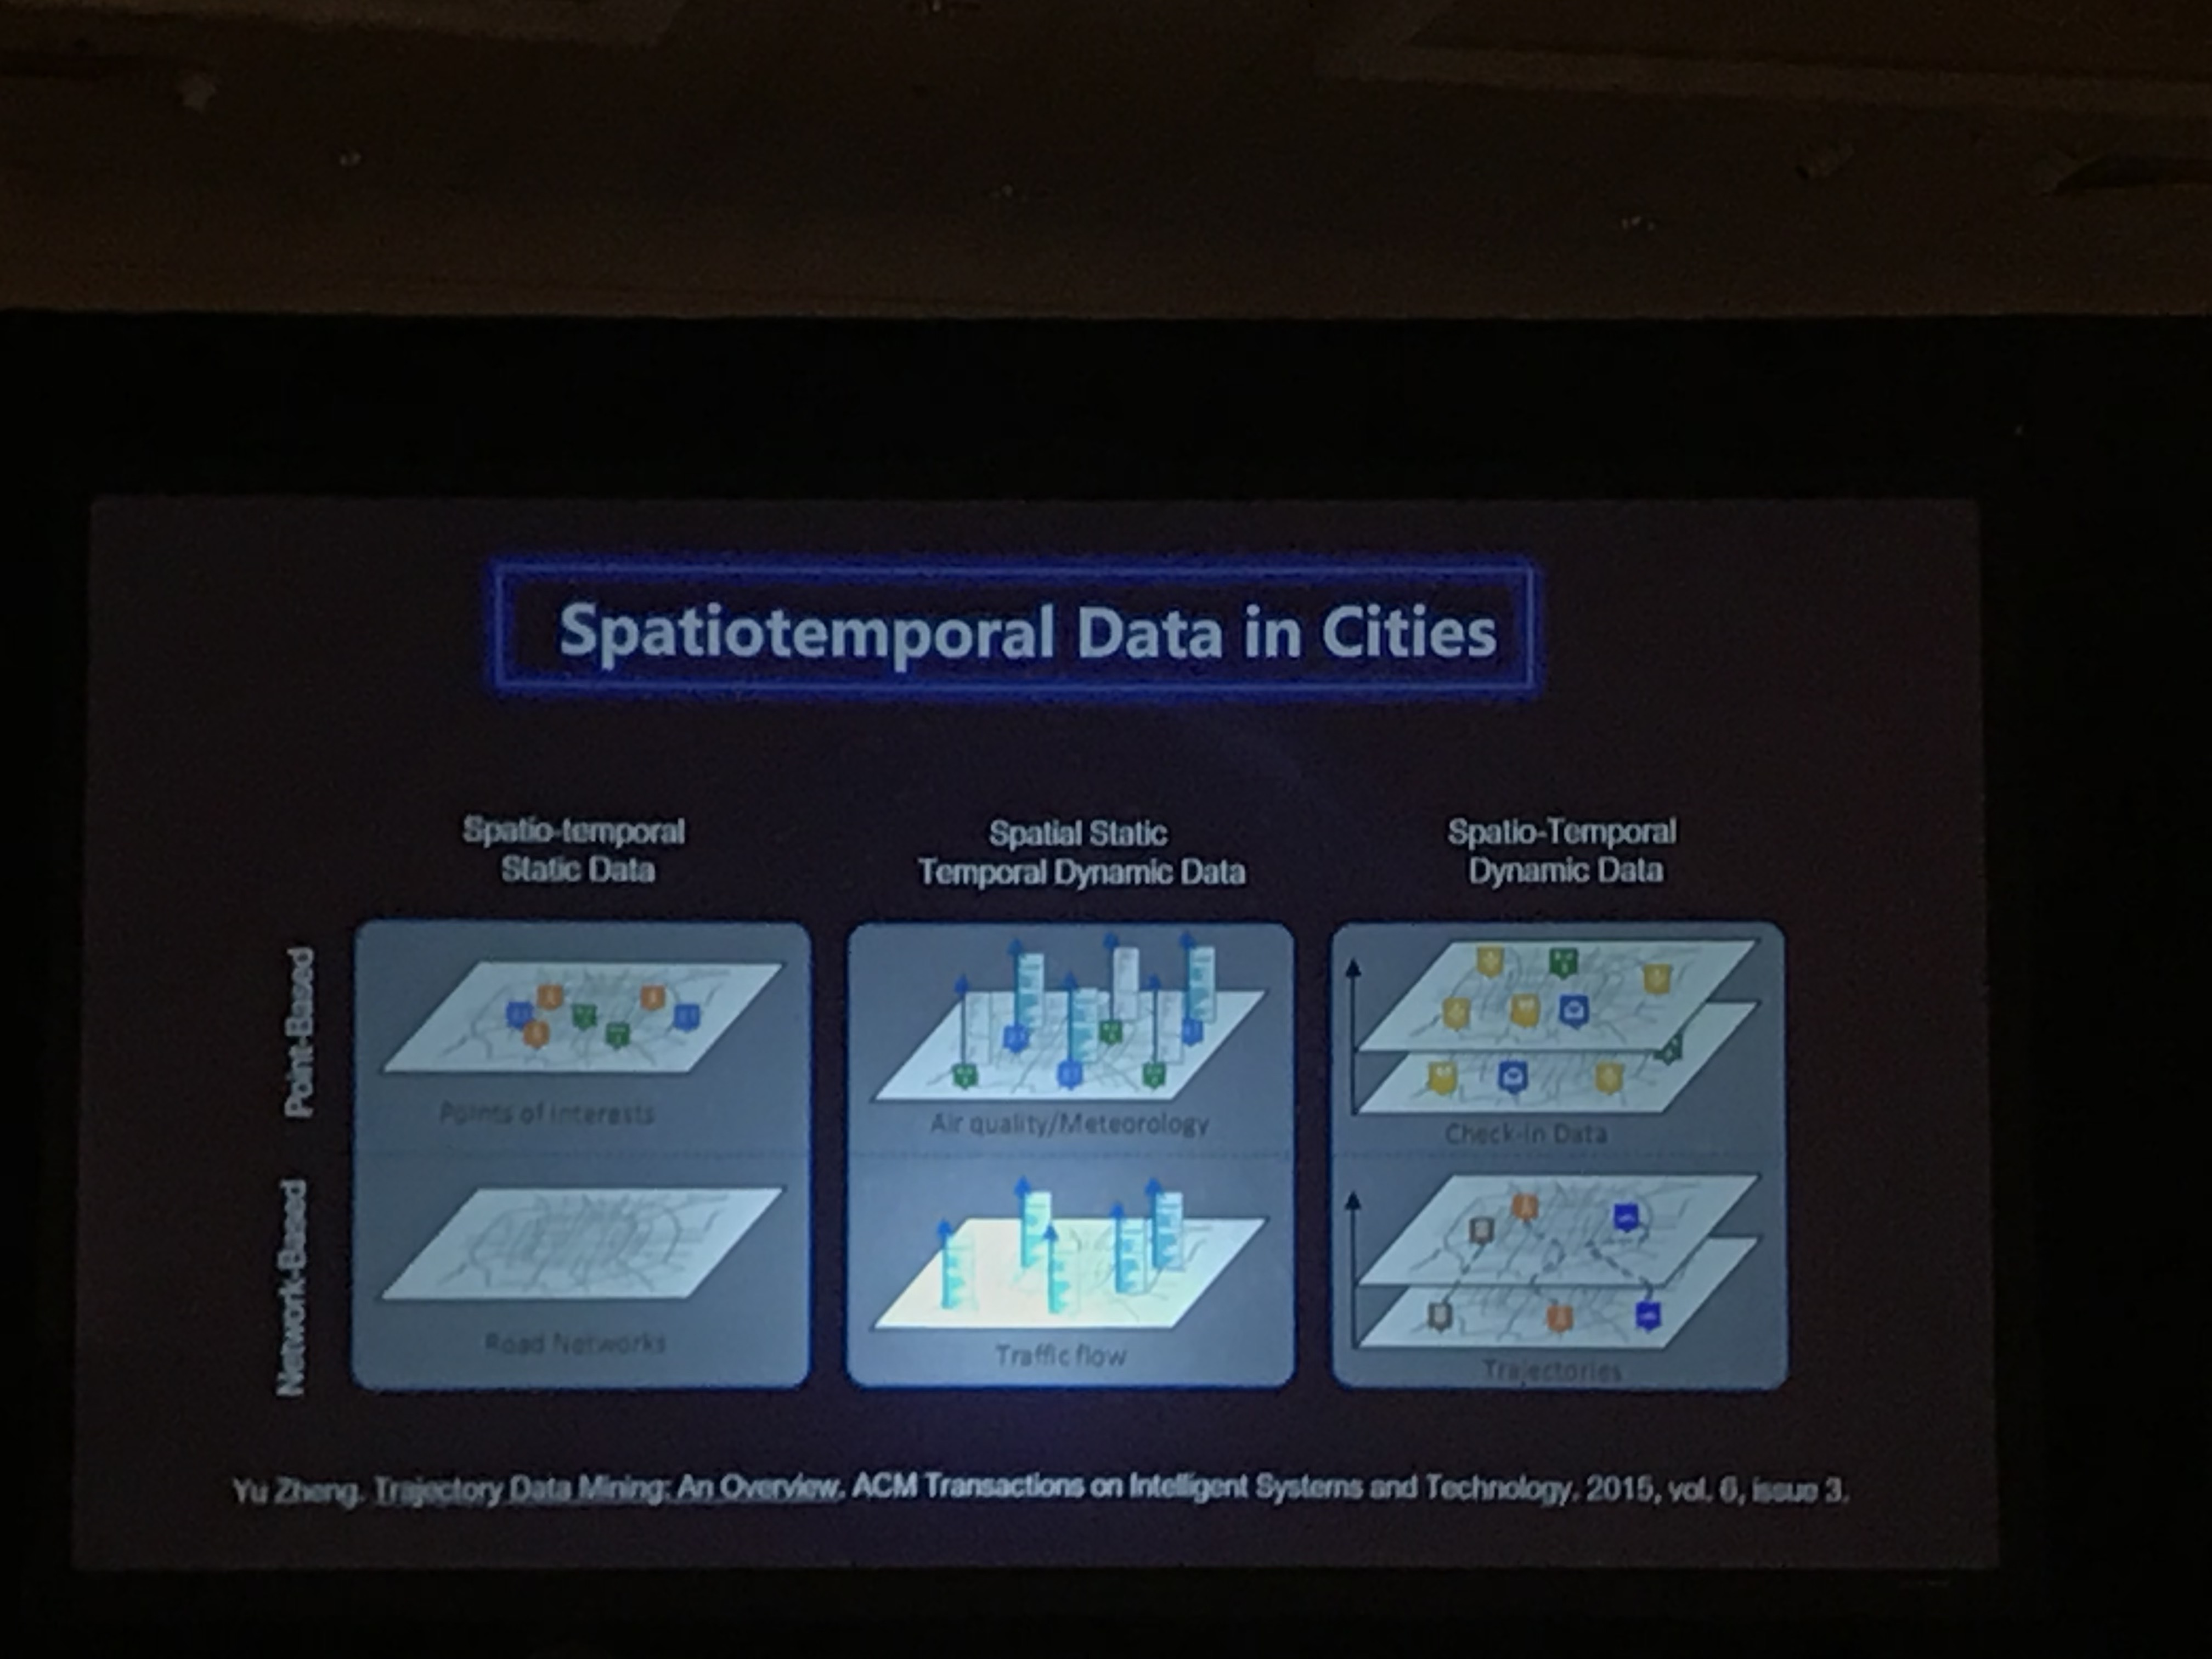
\includegraphics[width=0.5\textwidth]{images/data_type.JPG}
    \caption{Categorization of kinds of data in urban computing, designed to scale with new types of cities/data/challenges.}
    \label{fig:data_type}
\end{figure}

Spatiotemporal data is unique:
\begin{itemize}
    \item Spatial properties like distance, correlation. We can even apply triangle inequality.
    \item Spatial hierarchy: different spatial/geographic granularities, such as buildings $\in$ neighborhoods $\in$ districts.
    \vspace{2mm}
    \item Temrporal closeness, period, and trend give us further structure to exploit.
\end{itemize}

\subsubsection{Challenge 2: Data Management}

{\bf Problem:} large scale (city level!). So we need to handle a huge volume of data efficiently. \\

Hard to handle spatiotemporal data in particular:
\begin{itemize}
    \item Trajectory data is represented by a sequence of data types is highly complex.
    \item Unique queries make searching the data difficult.
    \item Data is spread across different domains, so requires hybrid indexing for maning multi-modal data.
\end{itemize}

Example: detect vehicle illegal parking using bike-share trajectories. \\

$\ra$ Solution: Can spot when bikes take odd swerves on a road to estimate where cars might be parked illegally~\cite{he2018detecting}. Use classification to spot the anomalous trajectories. \\


\subsubsection{Challenge 3: Data Analytics}

Example: Predicting crowd flows in a city. Difficult because of complex factors that effect this situation -- depends on time, events, weather, traffic, and so on. \\

$\ra$ Solution: partition a city into a uniform grid. Count the in flow and outflow of people in each grid cell over time. Now, given this series of grid-based-heat-maps, want to predict the grid at the next time-frame. Most off the shelf deep learning models don't capture the relevant spatio-temporal structure. Instead, develop a new architecture that looks for specific structure relevant to the domain~\cite{zhang2017deep}. \\

%\subsubsection{Mining Data from Different Domains}

{\bf Problem:} Air pollution is a global concern. Monitoring air quality is extremely difficult. \\

Solution: infer real-time and fine-grained air quality through a city~\cite{zheng2013u}. Provide a user interface for zooming in and out of a city to check the air quality at different regions of a city. Can even identify the source of solution. \\

$\ra$ Deployed in over 300 cities in china(!). Even offers prediction over the next 48 hours--\\

\subsubsection{Challenge 4: Providing Services}

Developed: urban computing platform that can accommodate the 6 types of data discussed previously, specially tuned for spatiotemporal data. \\

Opens up the opportunity for cities to share data and tools to improve inference and analytics. \\

Deployed: JD iCity, can play with it here: \url{http://ucp.jd.com} (\dnote{just a heads up it's in chinese}).

Summary:
\begin{itemize}
    \item Framework for urban computing
    \item Many research challenges, some effective solutions so far
    \item Urban computing platform as an OS for cities.
\end{itemize}

\spacerule

\subsection{Reasoning Under Uncertainty}

Now for some reasoning under uncertainty.


\subsubsection{On Testing of Uniform Samplers~\cite{chakraborty2019testing}}

Paper by Sourav Chakraborty and Kuldeep Meep. \\

Andrew Ng: ``AI is the new electricity" \\

And yet, it fails basic tasks: ``Im a huge metal fan" $\ra$ (translate to french) ``I'm a large ventilated object." \\

{\bf This Work:} Verification. \\

Given a model $M$, like a neural network to label images, and a specification, $\varphi$, that specifies the goals of $M$. \\

Idea of verification: We can check whether there exists an execution of $M$ that violates $\varphi$.\\

Q: Yes, but so what? \\

A: Well, samplers form the core of the state of the art probabilistic reasoning techniques. Can use Markov Chain Monte Carlo (MCMC). Use statistical test to argue for quality of the sampling distribution. \\

Example: suppose we're uniformly sampling from a domain from 1 to $N$. Distance is total variation distance ($\ell_1$). How many samples do we need before getting a collision?\\

\begin{theorem}
Testing whether a distribution is $\eps$-close to uniform has query complexity $\Theta(\sqrt{S}/\eps^2)$, with $S$ the size of the domain(?) \dnote{missed citation -- from another paper}.
\end{theorem}

\ddef{Conditional Sampling}{Given a distribution $D$ on domain $S$, one can specify:
\begin{itemize}
    \item Specify a set $T \subset D$
    \item Draw samples according to the distr. $D_T$, that is, $D$ under the condition that the samples belong to $T$.
\end{itemize}}

Clearly, such a sampling technique is {\it as powerful} by setting $T$ to the full support. But, what else can we do? \\

Sampling algorithm (for the two ``true" uniform and non-uniform case -- how can we determine which distr we are sampling from?):
\begin{itemize}
    \item Pick two elements uniformly at random $x,y$.
    \item In the case of the ``far" distribution, one of the elements will have Pr $0$, and the other $\Pr > 0$.
    \item Now a constant number of conditional samples is enough to identify that the distribution is not uniform.
\end{itemize}


Q: What about other distributions? \\

A: Need a few more tests, but largely same idea as the above. \\

Consider: uniform sampler for CNF formulas: Given a CNF formula $\phi$ and a CNF sampler $A$, that outputs a random solution of $\phi$.

\ddef{CNF Sampler}{A CNF-Sampler $A$ is a randomized algorithm that, given a $\phi$, outputs a random element of the set $S$, such that for any$x\in S$:
    \[
    Pr(A(\phi) = x) = \frac{1}{|S|}
    \]
}

Main problem: come up with a good CNF sampler. \\

Algorithm: Similar idea to before, yields the following main result:
\begin{theorem}
Given $\eps, \eta, \delta$, the number of samples the above their algorithm needs to accept/reject the formula,
\[
K = \tilde{O}\left(\frac{1}{(n-\eps)^4}\right),
\]
samples for any input formula $\phi$.
\end{theorem}

Experiments: compare different CNF sampling algorithms on a variety of benchmarks. \\

Conclusion:
\begin{itemize}
    \item Need methodological approach for verification of AI systems.
    \item Need to go beyond qualitative verification to probabilistic verification.
    \item Sampling is a crucial component of the state of the art probabilistic reasoning systems.
    \item This work: property testing meets verification, promise strong theoretical guarantees.
\end{itemize}




\spacerule
\subsubsection{Finding All Bayes Net Structures Near-Optimally~\cite{liao2018finding}}

Paper by Zhenyu Liao, Charupriya Sharma, James Cussens, and Peter van Beek. \\

\ddef{Bayes Nets}{A directed acyclic graph (DAG) that model a joint distribution over a set of random variables}

Bayes Nets can model conditional independence and causation, they can learn and model structure in data. \\

Structure Learning: learn a Bayes Net from data using a score-and-search approach, given training data of $N$ instances. \\

$\ra$ Lots of approaches to structure learning -- 1) consider space of all DAGs, 2) restrict your structure, or 3) consider only the best $k$-scoring DAGs.\\

Problem: restricting structure too much might limit the Bayes Net, if you don't limit it won't scale. \\

{\bf This Work:} Structure learning that fixes both of the above problems. \\

Main Results:
\begin{itemize}
    \item Propose a novel approach to model averaging inspired by approximation algorithms
    \item Approach only consider models that are optimal or near-optimal (in score).
    \item Prove this approach is efficient and can scale to much larger networks than the SOTA.
\end{itemize}

\ddef{$\eps$-BNSL}{Given $\eps > 0$, a dataset $I$ over variables $V$ and a scoring function $\sigma$, the $\eps$-Bayes Net Structure Learning (BNSL) problem finds all networks:
\[
OPT \leq score(G) \leq OPT + \eps,
\]
where $\eps = (\rho-1) OPT$.}

Problem closely related to Bayes Factor (BF), which can be interpreted as a measure for the relative success of a model to predict data. \\

Other problem: scaling. \\

$\ra$ Solution: prune the search space --
\begin{theorem}
(From~\citet{teyssier2012ordering}) Given a vertex and two parent sets $\Pi$ and $\Pi'$, we can prune the if $\Pi \subset \Pi'$ and $\sigma(\Pi) \leq \sigma(\Pi')$, then $\Pi'$ can be safely pruned.
\end{theorem}

This work extends this theorem to the $\eps$-optimal case:
\begin{theorem}
Given a vertex and two parent sets $\Pi$ and $\Pi'$ and $\eps \geq 0$, we can prune the if $\Pi \subset \Pi'$ and $\sigma(\Pi) + \eps \leq \sigma(\Pi')$, then $\Pi'$ can be safely pruned.
\end{theorem}

Experiments show that their approach both scales and achieves near-optimal scores.

\spacerule
\subsubsection{Rethinking the Discount Factor in RL~\cite{pitis2019rethinking}}

Paper by Silviu Pitis. \\

Original title: ``The MDP is all you need!" -- we think that MDPs can sufficiently account for all the modeling power that we need. \\

Set out to show that MDPs are sufficient for general intelligence by defining some axioms and deriving rational behavior in MDPs. But, I couldn't do it. So, instead I'll be talking about rethinking the discount factor. \\

Why like the MDP as a model?
\begin{itemize}
    \item Preferences induced by the discounted value function satisfy several notions of consistency (our axioms!)
    \item Fundamental theorem of Inverse RL -- any abirtrary behavior can be represented as the optimal policy in some MDP~\cite{ng2000algorithms}.
\end{itemize}

Q: So, why might the MDP fail to model preferences? \\

A1: Human preferences are complex -- maybe agent can't learn the ``optimal policy". \\

A2: We have good reason to model preferences with respect to suboptimal policies. \\

A3: Cliff example in this paper gives a numerical example of the above. \\

MDPs can't model {\it arbitrary} preferences. Let $A$ and $B$ be two events. Then:
\begin{align}
    ABAAAA > AAABAAAA  > AABAAAA,
\end{align}
can't be captured. But, it's irrational to do that anyway.\\

$\ra$ What we care about is capturing {\it rational} behavior. \\

\ddef{Rationality}{Characterized by axioms that we agree preferences should satisfy, as in the Von Neuman and Morgenstern axioms (Completeness, Transitivity, Independence, Continuity, and some time-axioms Irrelevance, Dynamic Consistency, and Impatience)}

This work: define rational preferences over actions, states, and policies. MDPs induce preferences according to:
\[
\text{if  } V^1(s_1) > V^2(s_2)\hspace{6mm} \text{then } (s_1, \pi_1) > (s_2, \pi_2)
\]

Main result:
\begin{theorem}
There exist $\mc{R} : S \times A \ra \mathbb{R}$ and $\Gamma: S \times A \ra \mathbb{R}^+$ such that for all $s,a,\pi$:
\begin{equation}
    U(s,a,\pi) = R(s,a) + \Gamma(s,a) \bE_{s'\sim T(s,a)}[U(s', \Pi)].
\end{equation}
\end{theorem}
Closest thing to the usual rationally result -- basically, we need to think about discount factor as a function of $(s,a)$ instead of being fixed. \\

Q: Given the observed behavior, what utility function (parameterized by both reward and discount), is being optimized? \\

A: Nice direction for future work!

\spacerule

\subsection{Invited Talk: Tuomas Sandholm on Solving Imperfect Information Games}

Note: most real-world applications are imperfect information games. \\

Recently achieved superhuman AI performance in imperfect information games. \\

Q: How do we do it? \\

A: Techniques for perfect information games won't work. But, can rely on application/task specific techniques! \\

{\bf Challenges:} 1) Uncertainty about what others and chance will do, 2) Hidden state, so we need to interpret signals and {\it use game theory}. \\

$\ra$ The game theory is critical! But, hard to scale computationally. So, major challenge is scaling the game theory. \\

Libratus overview pictured in Figure~\ref{fig:libratus}. \\

\begin{figure}[h!]
    \centering
    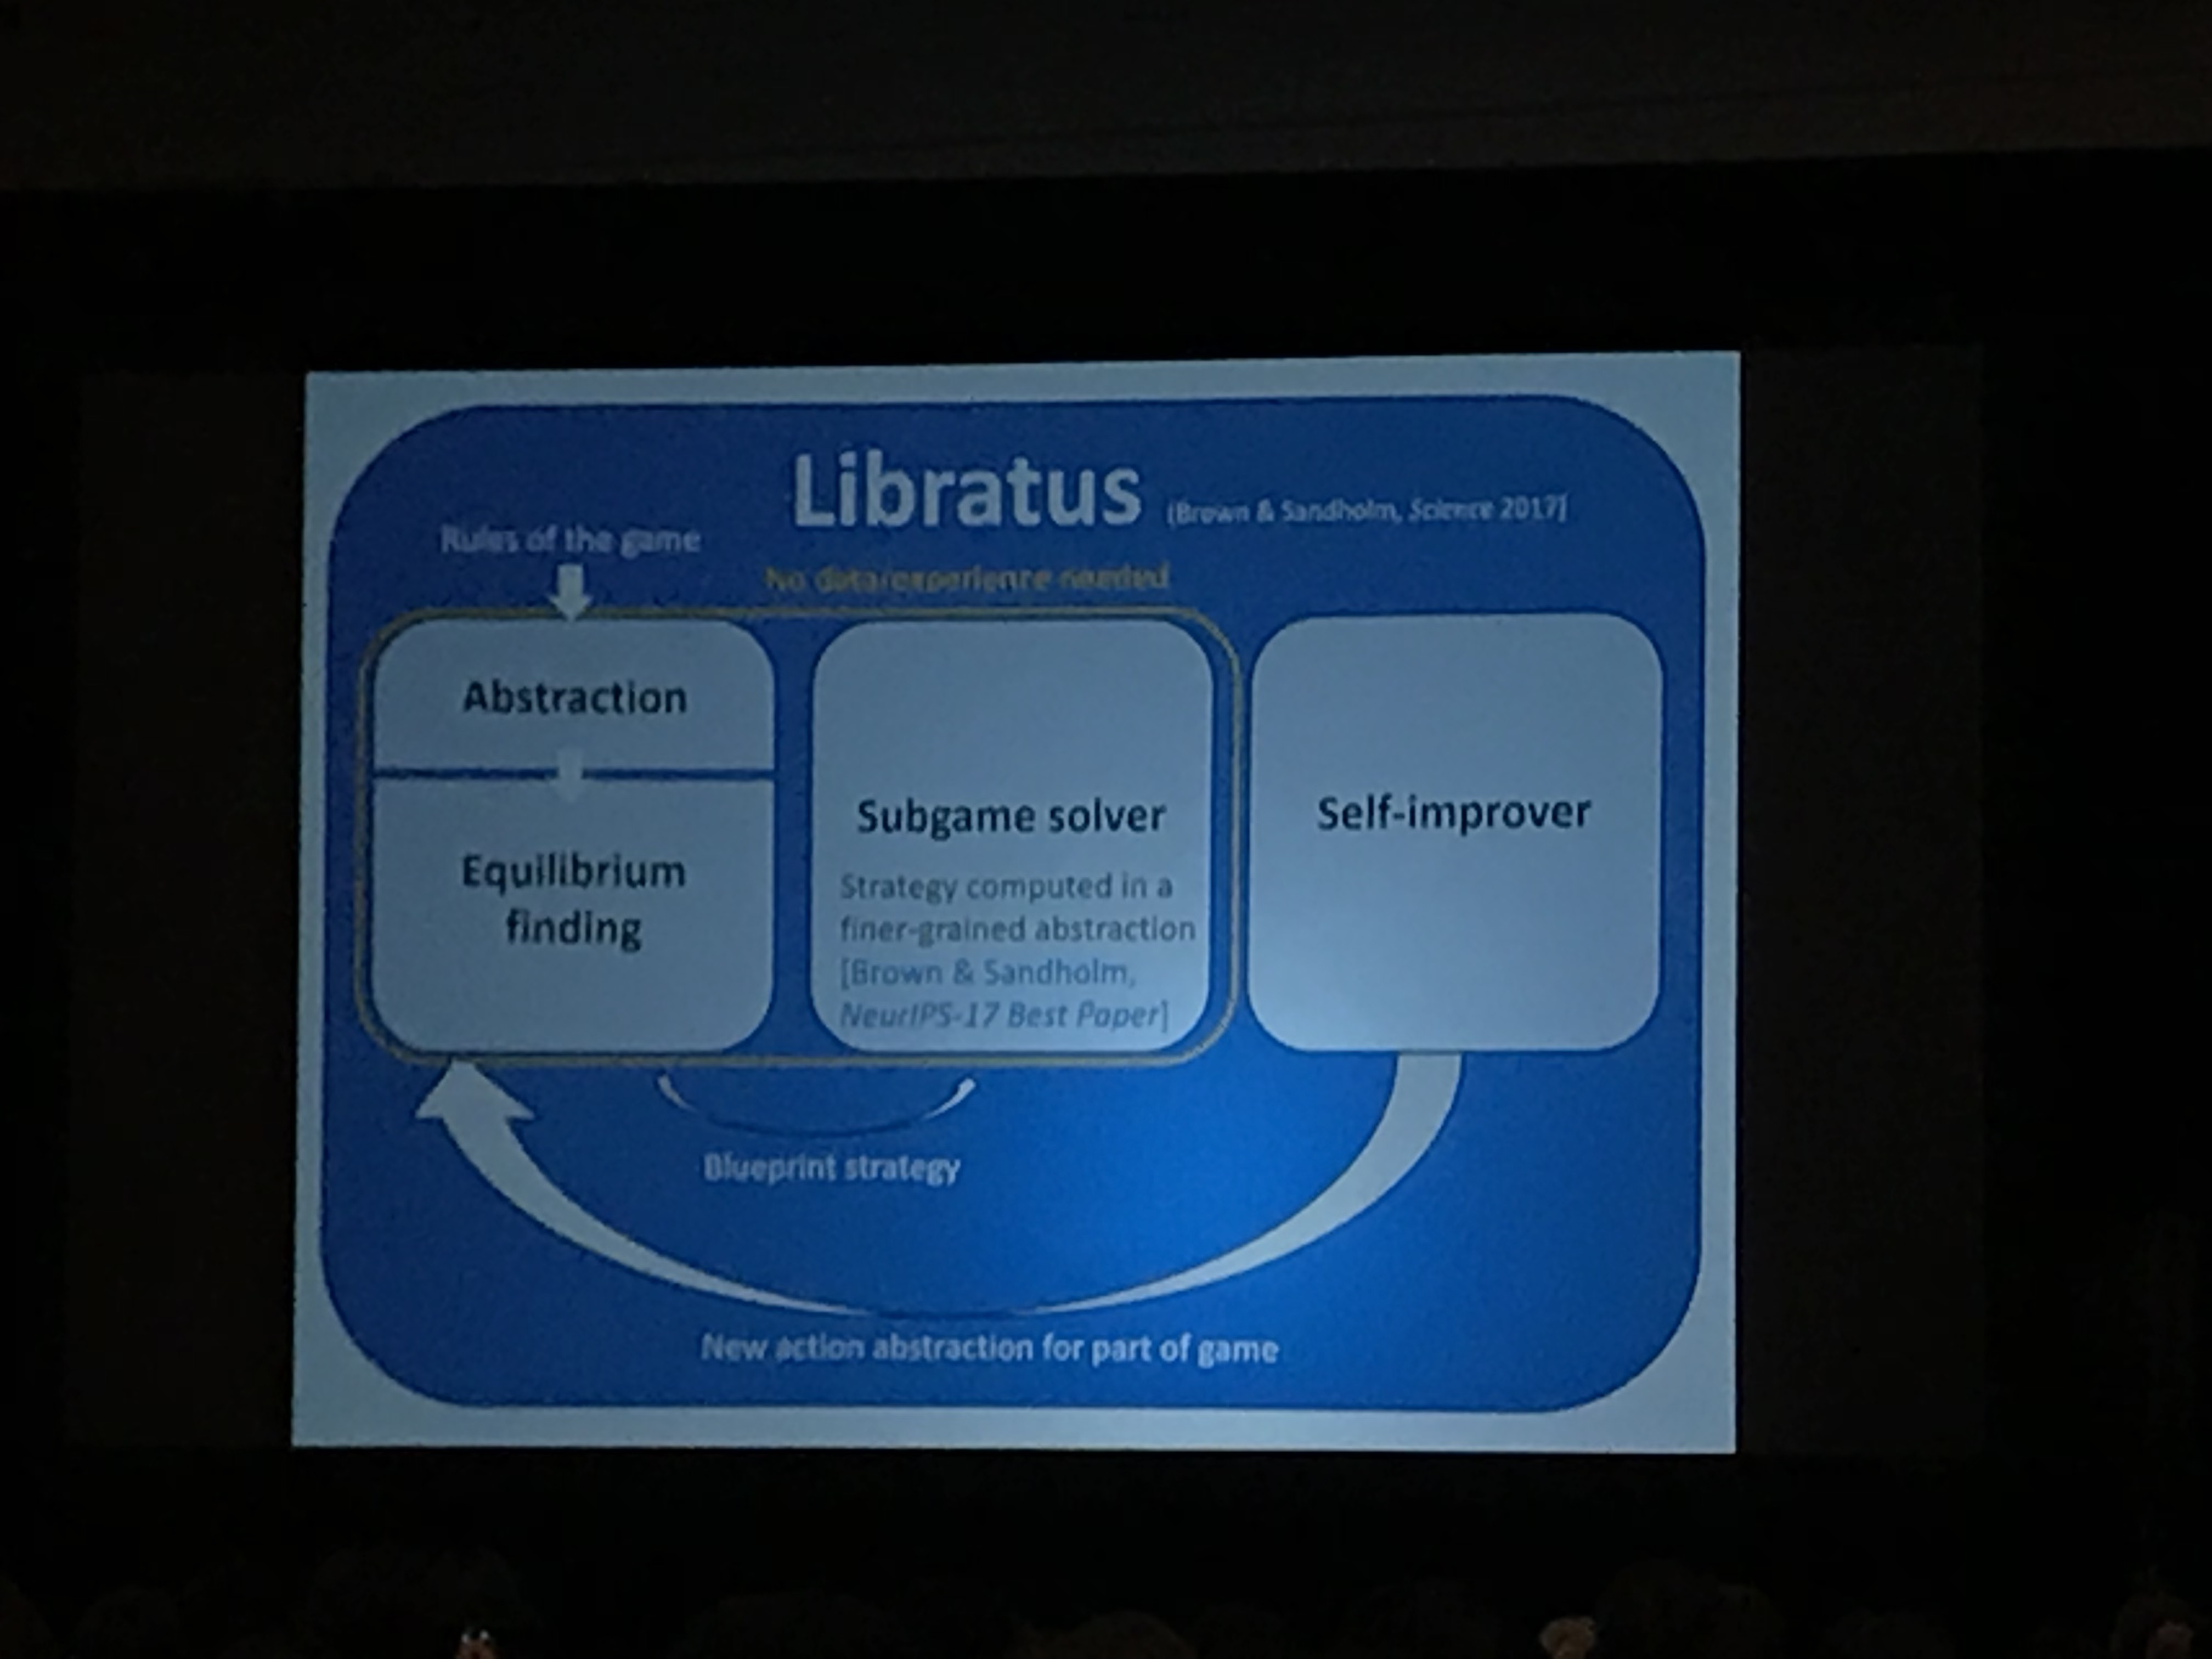
\includegraphics[width=0.5\textwidth]{images/libratus.JPG}
    \caption{Overview of Libratus.}
    \label{fig:libratus}
\end{figure}

\ddef{Extensive Form Game (EFG)}{Game with some chance and $N$ players is an extensive form game. Also defines a game tree of possibilities over plays, with payoff at the leaves (general sum).}

Strategies for EFG: behavioral strategy $\sigma_i$ with $i$ an information set. Specifies a distribution over actions. \\

Player $i$'s utility of strategy profile ($\sigma_1, \sigma_2)$. \\

$\eps$-Nash Equilibrium: strategy profile such that no player can improve behavior by more than $\eps$ by changing strategy. \\

Talk Roadmap:
\begin{itemize}
    \item Abstraction: unifed framework for game abstraction with solution quality bounds.
    \item Finding Nash Equilibrium: fast algorithms for solving games.
    \item Equilibrium Refinement
\end{itemize}

\subsubection{Abstraction}

Started with lossless absstraction~\cite{gilpin2007lossless} but, found we needed to move to lossy abstraction. Turns out abstraction in games in non-monotonic~\cite{waugh2009abstraction} \\

Q: Can we get bounds on solution quality anyway?  \\

A: Yes!~\cite{sandholm2012lossy}. Also applies to abstraction, since modeling is just abstraction. \\

Abstraction theorem:
\begin{theorem}
Given a perfect-recall game, an acylic abstract game, a mapping between the two games that satisfies mild assumptions, an $\eps$-Nash equilibrium in the abstract game, then: any lifted strategy is an $\eps$-Nash equilibrium in the original game:
\[
\eps' = \eps + \text{ mapping error } + \text{ refinement error.}
\]
\end{theorem}

Rest of the talk: theorems apply to 2-player, 0-sum games, but they're intended to apply to more general games. \\

Counterfactual regret minimization (CRM): used by every top poker AI in the past 5 years. Used a tabular form of CFR and abstraction before equilibrium finding. \\

$\ra$ Next up they introduce a function approximator for use in CRM. \\

Chicken-and-egg problem with abstractions: hard to pick an abstraction without knowing the equilibria, but hard to find the equilbiria without using an abstraction. \\

$\ra$ Solution: do both simultaneously! \\

Monto Carlo CRM~\cite{lanctot2009monte}:
\begin{itemize}
    \item Action regret is how much better we would have done had we alwasy picked this action in this situation in the past.
    \item Always pick action proportional to {\it positive regret}.
    \item 
\end{itemize}


% ------------
% -- Friday --
% ------------
\section{Thursday February 1st}
The final day! My talk is in the RL session this morning so I unfortunately didn't make it to the keynote.

\subsection{Reinforcement Learning}

First, some RL.

\subsubsection{Diversity-Driven Hierarchical RL~\cite{song2018diversity}}

Paper by Yuhang Song, Jianyi Wang, Thomas Lukasiewicz, Zhengua Xu, and Mai Xu. \\

Code at \url{github.com/YuhangSong/DEHRL} \\

{\bf Focus:} Hierarchical RL (HRL) \\

$\ra$ Idea: recombine sequences of basic actions to form sub-policies~\cite{sutton1999between}. \\

HRL can speed up learning, transfer, add explainability. \\

{\bf Game of Focus:} Overcooked. Cooking game where agents move around a grid and place objects in different locations subject to a timer. Need to place ingredients on certain objects (bread in toaster, etc.) with the goal of making food based on (randomly generated) orders given. \\

Task Features:
\begin{itemize}
    \item Primitive actions
    \item Abstract goals
    \item Sparse extrinsic reward (only received when agent collects the right ingredients based on the order
\end{itemize}

Using HRL on Overcooked: can use subpolicies to move agent in each direction, then higher level policies to move agent to each destination where ingredients can be collected/placed. \\

{\bf Main Idea:} Exploit and learn diversity driven policies for use in HRL. Comes from the following assumption:

\begin{assumption}
Learning different sub-policies is beneficial (popular in literature).
\end{assumption}

Their extension:
\begin{assumption}
With limited capability, learning sub policies far away from each one as possible is even better.
\end{assumption}

So, with this assumption, their solution:
\begin{itemize}
    \item Diversity of sub-policies can be measured by the {\bf distance} between the resulting states of sub-policies.
    
    \item Diversity-driven solution:
    
    $\ra$ Transition model memorize resulting states of different sub-policies
    
    $\ra$ Intrinsic reward generated based on if a sub-policy leads to a state that is far away from the resulting states if choosing another sub-policies.
\end{itemize}

Form a neural network that trains the many aspects of the above solution (models, policies, and so on). \\

Experiments (in Overcooked):
\begin{itemize}
    \item Sub-policy discovery at level 1 goes to the ``five most diverse/useful states" (out of around 600).
    \item At level 2, sub-policies fetch different ingredients at the four corners.
\end{itemize}

Experiments (in Minecraft) with no reward/supervision: goal is to break a block, build a block, or jump on a block.

$\ra$ Random policies can't do anything, but their HRL approach can actually build some nice structures. \\



\dnote{I'm up!}

\spacerule
\subsubsection{Towards Better Interpretability in DQN~\cite{annasamy2018towards}}

Paper by Raghuram Mandyam Annasamy and Katia Sycara. \\


{\bf Goal:} Interpretability! \\

$\ra$ Important for Deep RL since most neural nets used are treated as a black box, but naturally these systems will be deployed in crucial areas soon. \\

Lots of examples of seeking interpretability in supervised learning. But, it's harder in Deep RL\\

Proposed Method: ``interpretable"-DQN. Keys initialized randomly and learned via backprop. \\

Four loss functions:
\begin{itemize}
    \item Bellman Error (for $Q$ Learning)
    \item Distributional Error (force good representations/robustness \dnote{I think, missed this one})
    \item Reconstruction Error (force interpretable)
    \item Diversity Error (force attention)
\end{itemize}

Intuition:
\begin{itemize}
    \item Use key-value pairs to enforce interpretability.
    \item Keys act like cluster-centers
    \item Can then evaluate/visualize these cluster centers through things like t-sne.
    \item Pass keys through conlutional network to generate canonical states
\end{itemize}

Evaluation:
\begin{itemize}
    \item ``Agreement metric" used for evaluating the approach.
    \item Induce new distribution in image space.
    \item Random agreement will be around $1/|A|$.
    \item In Pac-Man they find 30\% agreement vs the random (which is roughly 10\%).
\end{itemize}

Examples of memorization: Create small permutations to existing states and test what the agent does. \\

Provide an interface for visualizing the reconstructions when small changes are made to the image. Find their i-DQN can do a good job of ignoring the perturbations. \\

{\bf Problem:} Lots of Deep RL methods overfit!~\cite{cobbe2018quantifying,zhang2018dissection}. Can use i-DQN to explore this a bit. 



\spacerule
\subsubsection{On RL for Full-Length Game of Starcraft~\cite{pang2018reinforcement}}

Paper by Zhen-Jia Pang, Ruo-Ze Liu, Zhou-Yu Meng, Yi Zhang, Yang Yu, and Tong Lu. \\

Why Starcraft?
\begin{itemize}
    \item Game is ideal for RL
    \item Most successful real time strategy of all time
    \item Really hard for human and AI to play
    \item If SC is solved, most games can be solved
\end{itemize}

\ddef{Starcraft}{Starcraft is a game where you control a base, units, and manage resources. You must build up a base and good units to destroy the other enemies.}

Difficulties: Starcraft can be multi-agent, is partially observable, and requires both macro level reasoning and low level control over many units. \\

Main focus: massive state-action space {\it and} long horizon until receiving reward. So, how can we solve this? \\

Approach:
\begin{itemize}
    \item Low-level abstraction: build a building (select unit $\ra$ build building $\ra$ go back to work), or produce a unit (select building, etc.).
    
    $\ra$ Can be inferred from mirroring human demonstrations, gives rise to macro-actions.
    
    \item High-level abstraction: Learn high level policies over these macro-actions (the ``low-level" abstractions).
\end{itemize}

Experiments:
\begin{itemize}
    \item Map: simple64
    \item Enemy: Terrain (built in AI)
    \item Agent: Protoss
    \item Fixed types of units/buildings for agent (but not enemy).
    \item High level policy that is decomposed into:
    \begin{enumerate}
        \item a ``base" policy responsible for handling base building and resource management.
        \item a ``battle" policy responsible for dealing with battle/focused on individual control.
    \end{enumerate}
\end{itemize}

Conclusions: 1) Investigate hierarchical architecture for SC, 2) Simple yet effective training algorithm, and 3) Achieves SOTA results on SC. \\


\spacerule

\subsection{Reasoning under Uncertainty}

Next some reasoning under uncertainty.

\subsubsection{Collecting Online Learning of GPs in Multi-Agent Systems}

Paper by Nghia Hoang, Quang Minh Hoang, Bryan Kian Hsiang Low, and Jonathon How. \\

Collecting Learning Motivation:
\begin{itemize}
    \item Local agents that can upload local statistics
    \item Old approach: Central server combine and broad cast
    $\ra$ But, limitation of typical approaches: centralized risk of failure and communication/computational bottleneck.
    
    \item Their approach fixes these shortcomings by removing central server. 
    
    $\ra$ No centralized risk of failure and no computational/communication bottlenecks.
\end{itemize}

Challenges: decentralization! Not clear how to do this (especially with resource constraints). \\

{\bf Goal:} Develop efficient local model representation for online update with data. \\

Gaussian Process (GP prediction is {\it not efficient}:
\begin{itemize}
    \item Computation is cubis
    \item Representation is quadratic
    \item Update is cubic
\end{itemize}

Solution: exploit sparse coding $\bm{u} = u(Z)$ is distributed by a standard GP. \\

Q: How can agent share models without communicating raw data? \\

A: Do local (bayesian/GP) updates, then share a representation that merges these updates. Main idea is to exploit additive structure to make this shared representation from a few messages.\\


Experiments: test on (real-world) traffic data set, characterizes different traffic phenomena. \\

$\ra$ Finding: they can reduce error with more data efficiently. 


\spacerule


\subsubsection{Weighted Model Ingeration using Knowledge Compilation}

Paper by Pedro Zuidberg Dos Martiers, Anton Dries, and Luc de Raedt. \\

{\bf Setting:} Probabilistic inference.  Goal is to combine the best of continuous and discrete inference \\

Knowledge compilation: take a boolean formula, compile it offline line so that you can do quick inference online. \\

New Method that can handle all of 1) knowledge compilation, 2) inference of density functions, 3) exact and approximate inference, and 4) can handle poly-nomial or non-linear constraints. \\

{\bf Contribution:} Can handle probability density functions while applying state of the art knowledge compilation techniques, along with two new solvers: Symbo and Sampo. \\

Symbo does: 1) abstract theory, 2) compile formula, 3) to arithmetic circuit, 4) label leaves, 5) evaluate, 6) multiply by weight of continuous variables, 7) integrate. \\

Sampo does: approximate Monte Carlo inference for doing approximate probabilistc inference with linear time dependency.  First sampling based algorithm for ``WMI"\\

$\ra$ Both samplers beat state of the art.


\dnote{Back to RL}

\subsubsection{Off-Policy Deep RL by Bootstrapping the Covariate Shift}

Paper by Carles Gelada and Marc Bellemare. \\

TD Policy Evaluation with Linear models: samples $s \sim d_\pi, a \sim \pi, r = R(s,a), s' \sim P(\cdot \mid s, a)$. \\

Linear value approximation $V_k(s) = \phi(s) \theta_k$. \\

Weight update:
\[
\theta_{k+1} \la \theta_k + \alpha(r + \gamma V_k(s') - V_k(s)) \phi(s).
\]
Can treat the above weight update as application of an operator. \\

Idea: also do {\it projection} operator this way: $\Pi_{d_\pi} x$. Well known result that Bellman operator converges. \\

{\bf Off Policy Problem:} End up with a {\it different} operator that does not lead to convergence. Well know difficulty from Baird (Baird's counter example)~\cite{baird1995residual}. \\

\ddef{Covariate Shift}{Sample from another distribution $\mu$, induces the covariate shift: $\frac{d_\pi(s)}{d_\mu(s)}$.}

Yields an update rule defined by this ratio, gives an operator:
\[
C_{k+1} = \Pi_{d_\mu} Y c_k.
\]
which {\it does} converge. But, it might converge to bad behaviour. \\

Idea: Can treat this as a projection into a simplex, which lets them translate the above new update rule to cooperate with neural networks. \\

Interpretation of the discount here: discounted of value function relxas the operator $P_\pi$ to $\gamma P_\pi$. Similarly, treat operator $Y$ as relaxing $P_\pi$ to $\gamma P_\pi + (1-\gamma) ed_\mu$. \\

{\bf Result:} $N$ step contraction factor under the discounted operator $\gamma Y$. 

\begin{theorem}
For any $n$, for any $\gamma$, can find an operator $Y$ that converges to a fixed point.
\end{theorem}

Experiment with the C51 agent (the distr. RL agent). Evaluate in ``extreme off policy tasks"), like seaquest. \\

\dnote{Back to reasoning under uncertainty.}




\spacerule
\subsubsection{Compiling Bayes Net Classifiers into Decision Graphs~\cite{shih2019compiling}}

Paper by Andy Shih, Arthur Choi, and Adnan Darwiche. \\

{\bf Goal:} Compile a (Bayes Net) classifier into a decision graph to better explain a classifier. \\


Case study: win95pts. \\

$\ra$ consider a printer with some symptons (slow printing, low toner, etc.). \\

Two kinds of explanations: can you fix a set of features such that the remaining features are rirrelevant, or can we remove erreoneous features. \\

{\bf Compilation:}
\begin{enumerate}
    \item Insight 1: recursively decompose into subclassifiers.
    \item Insight 2: Identify subclasiffiers that are equivalent to save computation time.
\end{enumerate}

Q: How can we. given two subclassifiers $B_1$ and $B_2$, identify  if $\forall_{v \in V} B_1(v) = B_2(v)$. \\

A: Goal is to compute $\Pr(C = 1 \mid v) \geq T$, which we can rewrite as a linear inequality. Problem becomes separating points on a line, so we binary search in time $O(|V|)$. \\

Experiments: use classifiers from literature that we can compile successfully into small ODDs. Try win95pts, Andes, cpcs54 $\ra$ they can all be merged and reduced quite dramatically. \\

Scaled this to networks with over 40 features. \\

{\bf Takeaways:}
\begin{itemize}
    \item Classifiers have an underlying decision function
    \item Decision functions can be compiled into an ODD
    \item Explanations and verification are efficient on ODDs (which are otherwise intractable on Bayesian network classifiers).
\end{itemize}



% --- Bibliography ---
\bibliographystyle{plainnat}
\bibliography{aaai}

\end{document}